%	-------------------------------------------------------------------------------
% 
%
%
%
%
%
%
%
%
%
%	-------------------------------------------------------------------------------
%	\documentclass[12pt, a4paper, twoside]{book}
%	\documentclass[12pt, a4paper, twoside, openright]{book}
	\documentclass[12pt, a4paper, oneside]{book}
%	\documentclass[12pt, a4paper, landscape, oneside]{book}

		% --------------------------------- 페이지 스타일 지정
		\usepackage{geometry}
%		\geometry{landscape=true	}
		\geometry{top 		=10em}
		\geometry{bottom		=10em}
		\geometry{left		=8em}
		\geometry{right		=8em}
		\geometry{headheight	=4em} % 머리말 설치 높이
		\geometry{headsep		=2em} % 머리말의 본문과의 띠우기 크기
		\geometry{footskip		=4em} % 꼬리말의 본문과의 띠우기 크기
% 		\geometry{showframe}
	
%		paperwidth 	= left + width + right (1)
%		paperheight 	= top + height + bottom (2)
%		width 		= textwidth (+ marginparsep + marginparwidth) (3)
%		height 		= textheight (+ headheight + headsep + footskip) (4)



		%	===================================================================
		%	package
		%	===================================================================
%			\usepackage[hangul]{kotex}				% 한글 사용
			\usepackage{kotex}						% 한글 사용
			\usepackage[unicode]{hyperref}			% 한글 하이퍼링크 사용
			\usepackage{amssymb,amsfonts,amsmath}	% 수학 수식 사용

			\usepackage{scrextend}					% 
		
		% ------------------------------ 개조식 문서 작성
			\usepackage{enumerate}			%
			\usepackage{enumitem}			%
			\usepackage{tabto}				%     tabto package
			\usepackage{tablists}			%	수학문제의 보기 등을 표현하는데 사용
										%	tabenum




		% ------------------------------ box & minipage
			\usepackage{setspace}			%
			\usepackage{booktabs}			% table
			\usepackage{color}				%
			\usepackage{boxedminipage}		% 미니 페이지
			\usepackage[pdftex]{graphicx}	% 그림 사용
			\usepackage[final]{pdfpages}	% pdf 사용
			\usepackage{framed}			% pdf 사용
			
			\usepackage{fix-cm}	
			\usepackage[english]{babel}
	
			\usepackage{tikz}%
			\usetikzlibrary{arrows,positioning,shapes}
			%\usetikzlibrary{positioning}

		% ------------------------------ 그림
			\usepackage[pdftex]{graphicx} 	% 그림
			\usepackage{floatflt} 			% 그림
			\usepackage{subfigure} 		% 그림
			\usepackage{pdfpages} 			% 그림
			


		%	=======================================================================================
		% 	tikz package
		% 	
		% 	--------------------------------- 	
			\usepackage{tikz}%
			\usetikzlibrary{arrows,positioning,shapes}
			\usetikzlibrary{mindmap,trees}			
		%	=======================================================================================
		% 	mdframed package
		% 	
		% 	--------------------------------- 	
			\usepackage[framemethod=TikZ]{mdframed}				% md framed package
			\usepackage{smartdiagram}							% smart diagram package


		% ------------------------------ table 
			\usepackage{longtable}			%
%			\usepackage[table]{xcolor}		 xcolor 이 충돌을 자꾸 일으킴
			\usepackage{rotating}
			\usepackage{array}
			\usepackage{tabularx}
			\usepackage{tabulary}
			\usepackage{multirow}

			\usepackage{tabu}				%
			\usepackage{tabto}				%  tabto package  
%			\usepackage{subcaption}		%  sub caption package  : 다중 캡션  subfigure와 충돌됨


		% --------------------------------- 	page
			\usepackage{afterpage}			% 다음페이지가 나온면 어떻게 하라는 명령 정의 패키지
%			\usepackage{fullpage}			% 잘못 사용하면 다 흐트러짐 주의해서 사용
%			\usepackage{pdflscape}			% 
			\usepackage{lscape}			%	 


			\usepackage{blindtext}
			\usepackage{lipsum}
	
		% --------------------------------- 특수문자 font 사용
			\usepackage{pifont}			%
			\usepackage{textcomp}
			\usepackage{gensymb}
			\usepackage{marvosym}



			\usepackage[cc]{titlepic}  		% 표지에 그림 넣기 위한 패키지
			\usepackage{listings}			%
			





		% --------------------------------- 페이지 스타일 지정

		\usepackage[Sonny]		{fncychap}

			\makeatletter
			\ChNameVar	{\Large\bf}
			\ChNumVar	{\Huge\bf}
			\ChTitleVar	{\Large\bf}
			\ChRuleWidth	{0.5pt}
			\makeatother

%		\usepackage[Lenny]		{fncychap}
%		\usepackage[Glenn]		{fncychap}
%		\usepackage[Conny]		{fncychap}
%		\usepackage[Rejne]		{fncychap}
%		\usepackage[Bjarne]	{fncychap}
%		\usepackage[Bjornstrup]{fncychap}

		\usepackage{fancyhdr}
		\pagestyle{fancy}
		\fancyhead{} % clear all fields
		\fancyhead[LO]{\footnotesize \leftmark}
		\fancyhead[RE]{\footnotesize \leftmark}
		\fancyfoot{} % clear all fields
		\fancyfoot[LE,RO]{\large \thepage}
		%\fancyfoot[CO,CE]{\empty}
		\renewcommand{\headrulewidth}{1.0pt}
		\renewcommand{\footrulewidth}{0.4pt}
	

		%	--------------------------------------------------------------------------------------- 
		% 	tritlesec package
		% 	
		% 	
		% 	------------------------------------------------------------------ section 스타일 지정
			\usepackage{titlesec}
		
		% 	----------------------------------------------------------------- section 글자 모양 설정
			\titleformat*{\section}					{\large\bfseries}
			\titleformat*{\subsection}				{\normalsize\bfseries}
			\titleformat*{\subsubsection}			{\normalsize\bfseries}
			\titleformat*{\paragraph}				{\normalsize\bfseries}
			\titleformat*{\subparagraph}			{\normalsize\bfseries}
	
		% 	----------------------------------------------------------------- section 번호 설정
			\renewcommand{\thepart}				{\arabic{part}.}
			\renewcommand{\thesection}				{\arabic{section}.}
			\renewcommand{\thesubsection}			{\thesection\arabic{subsection}.}
			\renewcommand{\thesubsubsection}		{\thesubsection\arabic{subsubsection}}
			\renewcommand{\theparagraph} 			{$\blacksquare$ \hspace{3pt}}

		% 	----------------------------------------------------------------- section 페이지 나누기 설정
			\let\stdsection\section
			\renewcommand\section{\newpage\stdsection}

		% --------------------------------- 	장, 절 등의 번호와 장, 절 등과의 간격 조정
		
			\titlespacing*{\section} 				{0pt}{1.0em}{1.0em}
			\titlespacing*{\subsection}	  		{0ex}{1.0em}{1.0em}
			\titlespacing*{\subsubsection}			{0ex}{1.0em}{1.0em}
			\titlespacing*{\paragraph}			{0ex}{1.0em}{1.0em}
			\titlespacing*{\subparagraph}			{0ex}{1.0em}{1.0em}

		% --------------------------------- recommend		섹션별 페이지 상단 여백
			\newcommand{\SectionMargin}			{\newpage  \null \vskip 2cm}
			\newcommand{\SubSectionMargin}		{\newpage  \null \vskip 2cm}
			\newcommand{\SubSubSectionMargin}		{\newpage  \null \vskip 2cm}



	
		% --------------------------------- mini toc 설정
			\usepackage{minitoc}


%		\renewcommand*{\partheadstartvskip}{\null\vskip20pt}
%		\renewcommand*{\partheadendvskip}{\vskip2pt}
%		\renewcommand\beforeparttoc{}		
		
		
		% --------------------------------- 절의 목차
		\setcounter{parttocdepth}{1}
		\setlength{\ptcindent}{0pt}
		\renewcommand{\ptcfont}{\normalsize\rm}
		\renewcommand{\ptcCfont}{\normalsize\bf}
		\renewcommand{\ptcSfont}{\normalsize\rm}
		
		% --------------------------------- 장의 목차
		\setcounter{minitocdepth}{1}    	% Show until subsubsections in minitoc
		\setlength{\mtcindent}{12pt} 		% default 24pt

	
	
		% --------------------------------- 	문서 기본 사항 설정
		\setcounter{secnumdepth}{4} 		% 문단 번호 깊이
		\setcounter{tocdepth}{3} 			% 문단 번호 깊이
		\setlength{\parindent}{0cm} 		% 문서 들여 쓰기를 하지 않는다.
		

		% --------------------------------- 	찾아보기
		\usepackage{makeidx}
		\makeindex

		% --------------------------------- 	줄간격 설정
		\doublespace
%		\onehalfspace
%		\singlespace
		
		
% 	============================================================================== List global setting
%		\setlist{itemsep=1.0em}
	
% 	============================================================================== enumi setting

%		\renewcommand{\labelenumi}{\arabic{enumi}.} 
%		\renewcommand{\labelenumii}{\arabic{enumi}.\arabic{enumii}}
%		\renewcommand{\labelenumii}{(\arabic{enumii})}
%		\renewcommand{\labelenumiii}{\arabic{enumiii})}


	%	-------------------------------------------------------------------------------
	%		Vertical and Horizontal spacing
	%	-------------------------------------------------------------------------------
		\setlist[enumerate,1]	{ leftmargin=8.0em, rightmargin=0.0em, labelwidth=0.0em, labelsep=0.0em }
		\setlist[enumerate,2]	{ leftmargin=8.0em, rightmargin=0.0em, labelwidth=0.0em, labelsep=0.0em }
		\setlist[enumerate,3]	{ leftmargin=8.0em, rightmargin=0.0em, labelwidth=0.0em, labelsep=0.0em }
		\setlist[enumerate]	{ 	itemsep=0.0em, 
								leftmargin=6.0ex, 
								rightmargin=0.0em, 
								labelwidth=0.0em, 
								labelsep=4.0ex 
							}


	%	-------------------------------------------------------------------------------
	%		Label
	%	-------------------------------------------------------------------------------
%		\setlist[enumerate,1]{ label=\arabic*., ref=\arabic* }
%		\setlist[enumerate,1]{ label=\emph{\arabic*.}, ref=\emph{\arabic*} }
%		\setlist[enumerate,1]{ label=\textbf{\arabic*.}, ref=\textbf{\arabic*} }   	% 1.
%		\setlist[enumerate,1]{ label=\textbf{\arabic*)}, ref=\textbf{\arabic*)} }		% 1)
		\setlist[enumerate,1]{ label=\textbf{(\arabic*)}, ref=\textbf{(\arabic*)} }	% (1)
		\setlist[enumerate,2]{ label=\textbf{\arabic*)}, ref=\textbf{\arabic*)} }		% 1)
		\setlist[enumerate,3]{ label=\textbf{\arabic*.}, ref=\textbf{\arabic*.} }		% 1.

%		\setlist[enumerate,2]{ label=\emph{\alph*}),ref=\theenumi.\emph{\alph*} }
%		\setlist[enumerate,3]{ label=\roman*), ref=\theenumii.\roman* }


	% 	============================================================================== itemi Global setting

	
		%	-------------------------------------------------------------------------------
		%		Vertical spacing
		%	-------------------------------------------------------------------------------
			\setlist[itemize]{topsep=0.0em}			% 상단의 여유치
			\setlist[itemize]{partopsep=0.0em}			% 
			\setlist[itemize]{parsep=0.0em}			% 
%			\setlist[itemize]{itemsep=0.0em}			% 
			\setlist[itemize]{noitemsep}				% 
			
		%	-------------------------------------------------------------------------------
		%		Horizontal spacing
		%	-------------------------------------------------------------------------------
			\setlist[itemize]{labelwidth=1em}			%  라벨의 표시 폭
			\setlist[itemize]{leftmargin=8em}			%  본문 까지의 왼쪽 여백  - 4em
			\setlist[itemize]{labelsep=3em} 			%  본문에서 라벨까지의 거리 -  3em
			\setlist[itemize]{rightmargin=0em}			% 오른쪽 여백  - 4em
			\setlist[itemize]{itemindent=0em} 			% 점 내민 거리 label sep 과 같은면 점위치 까지 내민다
			\setlist[itemize]{listparindent=3em}		% 본문 드려쓰기 간격
	
	
			\setlist[itemize]	{ 
						topsep=0.0em, 			%  상단의 여유치
						partopsep=0.0em, 		%  
						parsep=0.0em, 
						itemsep=0.0em, 
						labelwidth=1em, 
						leftmargin=2.5em,
						labelsep=2em,			%  본문에서 라벨 까지의 거리
						rightmargin=0em,		% 오른쪽 여백  - 4em
						itemindent=0em, 		% 점 내민 거리 label sep 과 같은면 점위치 까지 내민다
						listparindent=0em,		% 본문 드려쓰기 간격
						}

			\setlist[description]	{ 
							topsep=0.0em, 			%  상단의 여유치
							partopsep=0.0em, 		%  
							parsep=0.0em, 
							itemsep=0.0em, 
							labelwidth=1em, 
							leftmargin=2em,
							labelsep=1em,			%  본문에서 라벨 까지의 거리
							rightmargin=0em,		% 오른쪽 여백  - 4em
							itemindent=0em, 		% 점 내민 거리 label sep 과 같은면 점위치 까지 내민다
							listparindent=0em,		% 본문 드려쓰기 간격
							}

	%	-------------------------------------------------------------------------------
	%		Label
	%	-------------------------------------------------------------------------------
		\renewcommand{\labelitemi}{$\bullet$}
		\renewcommand{\labelitemii}{$\cdot$}
		\renewcommand{\labelitemiii}{$\diamond$}
		\renewcommand{\labelitemiv}{$\ast$}		




		% --------------------------------- recommend  글자 색깔지정 명령
		\newcommand{\red}		{\color{red}}			% 글자 색깔 지정
		\newcommand{\blue}		{\color{blue}}		% 글자 색깔 지정
		\newcommand{\black}	{\color{black}}		% 글자 색깔 지정
		\newcommand{\superscript}[1]{${}^{#1}$}

	
	
		% --------------------------------- 환경 정의 : 박스 치고 안의 글자 빨간색

			\newenvironment{BoxRedText}
			{ 	\setlength{\fboxsep}{12pt}
				\begin{boxedminipage}[c]{1.0\linewidth}
				\color{red}
			}
			{ 	\end{boxedminipage} 
				\color{black}
			}
			
			
			
		% --------------------------------- 예제를 위한 정의 


			\newenvironment{ex-001}{\textbf{연습문제}\begin{itshape}} {\end{itshape}}

			\newenvironment{env_ex-002}
			{ 	\setlength{\fboxsep}{12pt}
				\begin{boxedminipage}[c]{1.0\linewidth}
				\color{red}
			}
			{ 	\end{boxedminipage} 
				\color{black}
			}

			

% ------------------------------------------------------------------------------
% Begin document (Content goes below)
% ------------------------------------------------------------------------------
	\begin{document}
	
		% ----------------------- 장 목차 생성 Initialization
			\noptcrule 	% part toc에서 줄이 침범하는 에러가 나서 줄긋기를 중지 시킴			
			\dominitoc 		
			\doparttoc
			\dopartlof
			\dopartlot
			
			

	% 	--------------------------------------------------------- Title Page  Begin [ 약표제지 ]
		\begin{titlepage}
			\centering
			\null
			\vspace{2cm}
			{사용설명서 \huge\bfseries \LaTeX 김대희} \par
			\titlepic{\includegraphics[width=4cm]{./fig/pic_symark.pdf}} 
			
		\end{titlepage}
		\newpage
		\thispagestyle{empty}
	
	
	% 	--------------------------------------------------------- Title Page [ 표제지 ]
		\clearpage
		\begin{titlepage}
			\centering
			\null
			\vspace{2cm}
			{사용설명서 \huge\bfseries \LaTeX 김대희} \par
			\vspace{2cm}
			{\Large 김대희\par}
			\vfill
			% Bottom of the page
			{\large 2016.8.15 \par}
			\vspace{2cm}
		\end{titlepage}
		\newpage
		\thispagestyle{empty}



		\title{\LaTeX 김대희}
		\author{김대희}
		\date{\today}
		\titlepic{\includegraphics[width=4cm]{./fig/pic_symark.pdf}} 
		\maketitle


		\newpage
		\singlespace
		\tableofcontents
		\doublespace
		
		\newpage
		\listoffigures
		
		\newpage
		\listoftables


			



% 	==============================================================================  style


		\mdfdefinestyle	{code_document} {
						outerlinewidth		=1pt			,%
						innerlinewidth		=2pt			,%
						outerlinecolor		=blue!70!black	,%
						innerlinecolor		=white 			,%
						roundcorner			=4pt			,%
						skipabove			=1.0em 			,%
						skipbelow			=1.0em 			,%
						leftmargin			=0em			,%
						rightmargin			=0em			,%
						innertopmargin		=1em 			,%
						innerbottommargin 	=1em 			,%
						innerleftmargin		=1em 			,%
						innerrightmargin	=1em 			,%
						backgroundcolor		=gray!4			,%
						frametitlerule		=true 			,%
						frametitlerulecolor	=white			,%
						frametitlebackgroundcolor=gray		,%
						frametitleaboveskip=0.4em 			,%
						frametitlebelowskip=0.4em 			,%
						frametitlefontcolor=white 			,%
						}




%	=========================================================================================================================================== part 사용하기전 기본 사항
	\addtocontents{toc} {\protect\newpage}
	\part{사용하기전 기본 사항}

			\parttoc
	%		\partlof
	%		\partlot
				
	




% 	====================================================================================================================== chapter
	\chapter{사용하기 전 }
	\minitoc				% Creating an actual minitoc


	\clearpage
% 	---------------------------------------------------------------------------------------------------------------------- section
	\section{한글 사용}

	
	LaTaX은 서유럽 언어를 중심으로 만들어졌기 때문에 한글을 구현하기 위해서는 파일과 명령어를 추가해야 한다.

	ko.Tex는 Unicode/UTF-8인코딩과 EUC-KR을 모두 지원하나 
	원칙적으로 향후 발전 방향은 Unicode로 합의 되었으므로 Unicode/UTF-8 인코딜만을 다룬다.
	
	
	
	
	
% --------------------------------------- section --------------
\newpage
\section{pdf 북마크 기능 사용}
\null

		
	\paragraph{pdf에서 북마크 기능을 사용하려면}
	pdf에서 북마크 기능을 사용하려면 다음의 명령어를 프리앰블에 추가해야 한다.\\
	\verb|\usepackage{kotex}| \\
	\verb|\usepackage[unicode]{hyperref}| 

% --------------------------------------- section --------------
\newpage
\section{치수 단위}
\null

		\begin{table}[hbp]
		\caption{치수}
		\centering
		\begin{tabular}{l  l  l }
		\toprule
		명령어 & 결과 \\
		\toprule
		pt		& \tiny결과 &\normalsize{결과}\\
		pc		& \scriptsize{결과} \\
		in  		& \footnotesize{결과} \\
		bp 		& \small{결과} \\
		cm  	& \normalsize{결과} \\
		mm  	& \large{결과} \\
		dd 		& \Large{결과} \\
		cc 		& \LARGE{결과} \\
		sp 		& \huge{결과} \\
		\bottomrule
		\end{tabular}%
		\end{table}%



		\begin{table}[h!]
		\begin{tabularx}{1.0\textwidth}{ r X }
		\toprule
		Abbreviation				&Definition \\
		\midrule
		pt						&A point, is the default length unit. About 0.3515mm \\
		mm						&a millimetre \\
		cm 						&a centimetre \\
		in						&an inch \\
		ex						&the height of an x in the current font \\
		em						&the width of an m in the current font \\
		\textbackslash columnsep	&distance between columns \\
		\textbackslash columnwidth	&width of the column \\
		\textbackslash linewidth	&width of the line in the current environment \\
		\textbackslash paperwidth	&width of the page \\
		\textbackslash paperheight	&height of the page \\
		\textbackslash textwidth	&width of the text \\
		\textbackslash textheight	&height of the text \\
		\textbackslash unitleght	&units of length in the picture environment. \\
		\bottomrule
		\end{tabularx}
		\end{table}







% --------------------------------------- section --------------
\newpage
\section{문서의 종류}
\null

	\begin{itemize}
		\item 	article
		\item 	report
		\item 	book
		\item 	letter
		\item 	beamer
		\item 	amsart : 간단한 수학문서
		\item 	amsbook : 수학책
		\item 	minimal
		\item 	slides
		\item 	standalone
	\end{itemize}



% 	======================================================================================================================  문서의 장절구분
	\chapter{문서의 장절 구분}



	% --------------------------------------- section --------------
	\newpage
	\section{장과 절에 번호 붙이기}
	\null


	\begin{itemize}
	\item	번호를 사용하는 방법
			\begin{framed}
			\verb|\setcounter{secnumdepth}{2}|
			\end{framed}

	\item	이름을 사용하는 방법
			\begin{framed}
			\verb|\setcounter{secnumdepth}{subsection}|
			\end{framed}
	\end{itemize}




		% -------------------------------------- page -------------------
			\subsection{문서의 장절 구분 레벨}
	
			\begin{table}[hbp]
			\centering 
			\begin{tabular}{ p{0.4\textwidth} p{0.2\textwidth} p{0.3\textwidth} }
			\toprule
			Command				&Level	&Comment\\
			\midrule
			\verb|\part|				&-1	&not in letters\\
			\verb|\chapter|			&0		&only books and reports\\
			\verb|\section|			&1		&not in letters\\
			\verb|\subsection|		&2		&not in letters\\
			\verb|\subsubsection|	&3		&not in letters\\
			\verb|\paragraph|		&4		&not in letters\\
			\verb|\subparagraph|		&5		&not in letters\\
			\bottomrule
			\end{tabular} 
			\end{table}
	
	
			\subsection{sec num depth}
	
	
	
			\subsection{toc depth}
	
	
	
	
		\newpage  \null
		% -------------------------------------- page -------------------
			\subsection{Section number Style}
			
			각 카운터는 기본 형식이 있습니다. 이러한 형식은 내부 LaTeX의 명령을 사용하여 지정됩니다.
			
			\begin{table}[hbp]
			\centering 
			\begin{tabular}{ p{0.4\textwidth} p{0.5\textwidth} }
			\toprule
			command	&Example\\
			\midrule
			\verb|\arabic|	&1, 2, 3 ...\\
			\verb|\alph|	 	&a, b, c ...\\
			\verb|\Alph|		&A, B, C ...\\
			\verb|\roman|	&i, ii, iii ...\\
			\verb|\Roman|	&I, II, III ...\\
			\verb|\fnsymbol|	&Aimed at footnotes; prints a sequence of symbols.\\
			\bottomrule
			\end{tabular} 
			\end{table}






			
			\newpage  \null
		% -------------------------------------- page -------------------
			\subsection{5. Hyperlinks to content}
	
	



% 	======================================================================================================================  문서의 구성
	\newpage
	\chapter{\TeX 문서 구성}


	% -------------------------------------- page -------------------
		\minitoc				% Creating an actual minitoc
		\doublespace





	% --------------------------------------- section --------------
	\newpage 
	\section{\TeX 문서의 구성}
	\null
	
			\TeX의 문서 구성은 
			\begin{itemize}
			\item 프리 앰블
			\item document
			\end{itemize}
			 로 구성된다.
	
	% --------------------------------------- section --------------
	\newpage
	\section{프리 앰블}
	\null
	
			프리앰블은 본문의 시작을 지시하는 \verb|\begin{document}|이전까지 
			문서 전체의 형식을 지정하는 부분이다.
		
	% --------------------------------------- section --------------
	\newpage
	\section{document}
	\null
	
	
	
	% --------------------------------------- section --------------
	\newpage
	\section{package}
	\null
	
			기본적인 패키지는 이미 설치되었을 것이지만, 직접 설치해야 하는 패키지가 있다. 
		
			가장 간단한 방법은 패키지를 사용하는 문서가 있는 폴더에 패키지 파일를 같이 두는 것이다.
		
			\paragraph{모든문서에서 사용하려면}
			모든문서에서 사용하려면 
			원하는 패키지를 다운받아 내장된 패키지 관리 유틸리티인 tlmgr을 사용하면된다.
		
			\paragraph{직접 설치하려면}
			직접 설치하고 싶다면 
			\verb|C:\user\texlive\2011\texmf-dist\tex\latex| 폴더 아래에하위 폴더를 만들면 된다.




%	=========================================================================================================================================== part 표지  목차 초록 찾아보기
	\addtocontents{toc} {\protect\newpage}
	\part{표지 목차 초록 찾아보기 }
	
			\parttoc
	%		\partlof
	%		\partlot




% 	====================================================================================================================== chapter  표지 제목 작성
	\chapter{표지 제목 작성}

	% -------------------------------------- page -------------------
		\minitoc				% Creating an actual minitoc
		\doublespace



	% --------------------------------------- section -------------- 
	\newpage  \null
	\section{제목, 저자, 작성일 작성}
		
		\begin{framed}
		\verb|\title{문서제목}| \\
		\verb|\author{저자}| \\
		\verb|\date{작성일, 별도 지정하지 않을 경우 컴파일한 날짜가 자동 생성됨}| \\
		\verb|\maketlitle|
		\end{framed}
	
	
	
	
	
	% --------------------------------------- section -------------- 
	\newpage  \null
	\section{표지에 그림 삽입 (titlepic)}
	
		\paragraph{패키지의 설치}
			표지에 그림을 삽입하려면 아래 두개의 패키지를 먼저 설치해야 한다.
			\begin{framed}
			\verb|\usepackage[cc]{titlepic}| \\
			\verb|\usepackage{graphicx}}|
			\end{framed}
	
		\paragraph{그림 삽입}
			본문에 titlepic명령 삽입
			\begin{leftbar}
			\verb|\title{문서제목}| \\
			\verb|\author{저자}| \\
			\verb|\date{작성일}| \\
			\verb|\titlepic{\includegraphics[width=2cm]{0000.png}}| \\
			\null \\
			\verb|\maketlitle|
			\end{leftbar}



% 	====================================================================================================================== chapter  초록
	\chapter{초록}

	% -------------------------------------- page -------------------
		\minitoc				% Creating an actual minitoc
		\doublespace
	
		
	% --------------------------------------- section -------------- 
	\newpage  \null
	\section{초록 작성}
	
	
	
	
	
	
% 	====================================================================================================================== chapter  목차
	\chapter{목차}

	% -------------------------------------- page -------------------
		\minitoc				% Creating an actual minitoc
		\doublespace


	
	
	% --------------------------------------- section -------------- 
	\newpage  \null
	\section{목차 작성}

			\begin{itemize}[topsep=0.0em, parsep=0.0em, itemsep=0em, leftmargin=6.0em, labelwidth=3em, labelsep=3em] 
			\item 	LaTeX에서는 아주 쉽게 목차를 만들 수 있다.
			\item 	다음의 영령어는 각각 본문 목차, 그림목차, 표목차를 생성하는 명령어이다. \\
					\textbf{본문} 목차 : \textbackslash tableofcontents \\
					\textbf{그림} 목차 : \textbackslash listoffigures \\
					\textbf{표} 목차 	: \textbackslash listoftables 
			\item 	\textbackslash maketitle 명령어 다음에 위의 명령어를 입력하고 두번 컴파일링 하면 된다.
			
			
			\end{itemize}
	
	
		\paragraph{□  목차의 작성} \tab
			\begin{framed}
			toc : \verb|\table of contents| \\
			lof : \verb|\list of figures| \\
			lot : \verb|\list of tables|
			\end{framed} 



	% --------------------------------------- section -------------- 
	\newpage  \null
	\section{본문 목차 \textbackslash table of contents}


	
	% --------------------------------------- section -------------- 
	\newpage  \null
	\section{그림 목차 \textbackslash list of figures}


	% --------------------------------------- section -------------- 
	\newpage  \null
	\section{표 목차 \textbackslash list of tables}



	% --------------------------------------- section -------------- 
	\newpage  \null
	\section{목차 작성의 범위 설정 \textbackslash setcounter }
	
		\subsection{□  목차 작성의 범위 설정}
			\begin{framed}
			\verb|\set counter { toc depth } { level } | 
			\end{framed}
			
			\vskip 4em
	
		\subsection{□  목차에서 목차 번호 설정 깊이 level }
			\begin{framed}
			\verb|\set counter { sec num depth } { n }| 
			\end{framed}

		%		\tabulinesep=0.6ex
				\begin{tabu} to 1.0\textwidth { X[r, 1.0] X[r, 1.0] X[c, 1.0]}
				\tabucline[0.2ex]{-}		
				부 		&part 			&-1 \\
				장 		&chapter 			&0 \\
				절 		&section 			&1 \\
				소절 	&subsection 		&2 \\
				소소절 	&subsubsection	&3 \\
				문단 	&paragraph 		&4 \\
				소문단 	&subparagraph 	&5 \\
				\tabucline[0.1ex]{-}		
				\end{tabu} 


	% --------------------------------------- section -------------- 
	\newpage  \null
	\section{목차에서 페이지 나누기  \textbackslash addtocontents }


		split the table of contents in two pages \\
		목차가 긴 경우 페이지를 나누어 줄려고 하는 경우
	
		\paragraph{□  목차에서 페이지 나누기} \tab
			\begin{framed}
			\verb|\add to contents { toc } { \protect \newpage }| 
			\end{framed}




	
		\newpage  \null
	% -------------------------------------- page -------------------
		
			

% ========================================== chapter ============
\newpage
\chapter{minitoc}
				
	% -------------------------------------- page -------------------
		%			\nomtcrule      		% removes rules = horizontal lines
		%			\nomtcpagenumbers  	% remove page numbers from minitocs
		%			\newpage
					\minitoc				% Creating an actual minitoc
					\doublespace

	% -------------------------------------------------------------
	\newpage
	\section{minitoc 개요}
	
	\subsection{문서의 처음에 선언}
	
				\begin{table}[h]
				\caption{minitoc 본문내에서 선언문}
				\centering 
				\tabulinesep=0.8ex
				\begin{tabu} to 0.8\textwidth { X[l, 1.0] X[l, 2] }
				\tabucline[0.2ex]{-}		
				\textbackslash doparttoc	&Table of contents for parts	\\
				\textbackslash dopartlof	&List of figures for parts	\\
				\textbackslash dopartlot	&List of tables for parts	\\
				\tabucline[0.1ex]{-}		
				\textbackslash dominitoc	&Table of contents for chapters	\\
				\textbackslash dominilof	&List of figures for chapters	\\
				\textbackslash dominilot	&List of tables for chapters	\\
				\tabucline[0.1ex]{-}		
				\textbackslash dosecttoc	&Table of contents for sections	\\
				\textbackslash dosectlof	&List of figures for sections	\\
				\textbackslash dosectlot	&List of tables for sections\\
				\tabucline[0.1ex]{-}		
				\end{tabu} 
		%		\label{table}
				\end{table}
				
	\subsection{문서내에서의 사용}

				\begin{table}[h]
				\caption{minitoc 본문내에서 사용문}
				\centering 
				\tabulinesep=0.8ex
				\begin{tabu} to 0.8\textwidth { X[l, 1.0] X[l, 2] }
				\tabucline[0.2ex]{-}		
				\textbackslash parttoc	&Table of contents for parts	\\
				\textbackslash partlof	&List of figures for parts	\\
				\textbackslash partlot	&List of tables for parts	\\
				\tabucline[0.1ex]{-}		
				\textbackslash minitoc	&Table of contents for chapters	\\
				\textbackslash minilof	&List of figures for chapters	\\
				\textbackslash minilot	&List of tables for chapters	\\
				\tabucline[0.1ex]{-}		
				\textbackslash secttoc	&Table of contents for sections	\\
				\textbackslash sectlof	&List of figures for sections	\\
				\textbackslash sectlot	&List of tables for sections \\
				\tabucline[0.1ex]{-}		
				\end{tabu} 
		%		\label{table}
				\end{table}





				
		\newpage
	% -------------------------------------------------------------
	\section{mini toc}
	
		%---------------
		\singlespace
		\setlength{\fboxsep}{12pt}
		\begin{boxedminipage}[c]{1.0\linewidth}
		\color{blue}
		%---------------
		\begin{verbatim}
			\documentclass[...]{book}
			\usepackage{minitoc}
			...
			\setcounter{minitocdepth}{2} default
			\setlength{\mtcindent}{24pt} default
			\renewcommand{\mtcfont}{\small\rm} default
			\renewcommand{\mtcSfont}{\small\bf} default
			...
			\begin{document}
			...
			\dominitoc
			\dominilof
			\dominilot
			\tableofcontents or \faketableofcontents
			\listoffigures or \fakelistoffigures
			\listoftables or \fakelistoftables
			...
			\chapter{...}
			\minitoc if you want one
			\minilof if you want one
			\minilot if you want one
			...
		\end{verbatim}
		%---------------
		\end{boxedminipage}
		\color{black}
		\doublespace
		%---------------

		
		\subsection{minitocdepth}
		
		
		\subsection{mtcindent}
				
								
		\subsection{dominitoc}

				
		\newpage
	% -------------------------------------------------------------
	\section{section toc }
	
		%---------------
		\singlespace
		\setlength{\fboxsep}{12pt}
		\begin{boxedminipage}[c]{1.0\linewidth}
		\color{blue}
		%---------------
		\begin{verbatim}
			\documentclass[...]{article}
			\usepackage{minitoc}
			...
			\setcounter{\secttocdepth}{2} default
			\setlength{\stcindent}{24pt} default
			\renewcommand{\stcfont}{\small\rm} default
			\renewcommand{\stcSSfont}{\small\bf} default
			...
			\begin{document}
			...
			\dosecttoc
			\dosectlof
			\dosectlot
			\tableofcontents or \faketableofcontents
			\listoffigures or \fakelistoffigures
			\listoftables or \fakelistoftables
			...
			\chapter{...}
			\secttoc if you want one
			\sectlof if you want one
			\sectlot if you want one
			...
		\end{verbatim}
		%---------------
		\end{boxedminipage}
		\color{black}
		\doublespace
		%---------------
		

		\subsection{secttocdepth}
		
		
		\subsection{stcindent}


		\subsection{dosecttoc}



		
		\newpage
	% -------------------------------------------------------------
	\section{part  toc }



		%---------------
		\singlespace
		\setlength{\fboxsep}{12pt}
		\begin{boxedminipage}[c]{1.0\linewidth}
		\color{blue}
		%---------------
		\begin{verbatim}
			\documentclass[...]{book}
			\usepackage{minitoc}
			...
			\setcounter{parttocdepth}{2} default
			\setlength{\ptcindent}{0pt} default
			\renewcommand{\ptcfont}{\normalsize\rm} default
			\renewcommand{\ptcCfont}{\normalsize\bf} default
			\renewcommand{\ptcSfont}{\normalsize\rm} default
			...
			\begin{document}
			...
			\doparttoc
			\dopartlof
			\dopartlot
			\tableofcontents or
			\faketableofcontents
			\listoffigures or
			\fakelistoffigures
			\listoftables or
			\fakelistoftables
			...
			\part{...}
			\parttoc if you want one
			\partlof if you want one
			\partlot if you want one
			...
		\end{verbatim}
		%---------------
		\end{boxedminipage}
		\color{black}
		\doublespace
		%---------------



		\newpage
	% -------------------------------------- page -------------------
		\subsection{part toc depth}
		
		
		\subsection{ptc indent}


		\subsection{do part toc}


		\subsection{part toc}
		

		\subsection{do part lof}

		\subsection{part lof}

		\subsection{do part lot}

		\subsection{part lot}






















	
			\cleardoublepage
			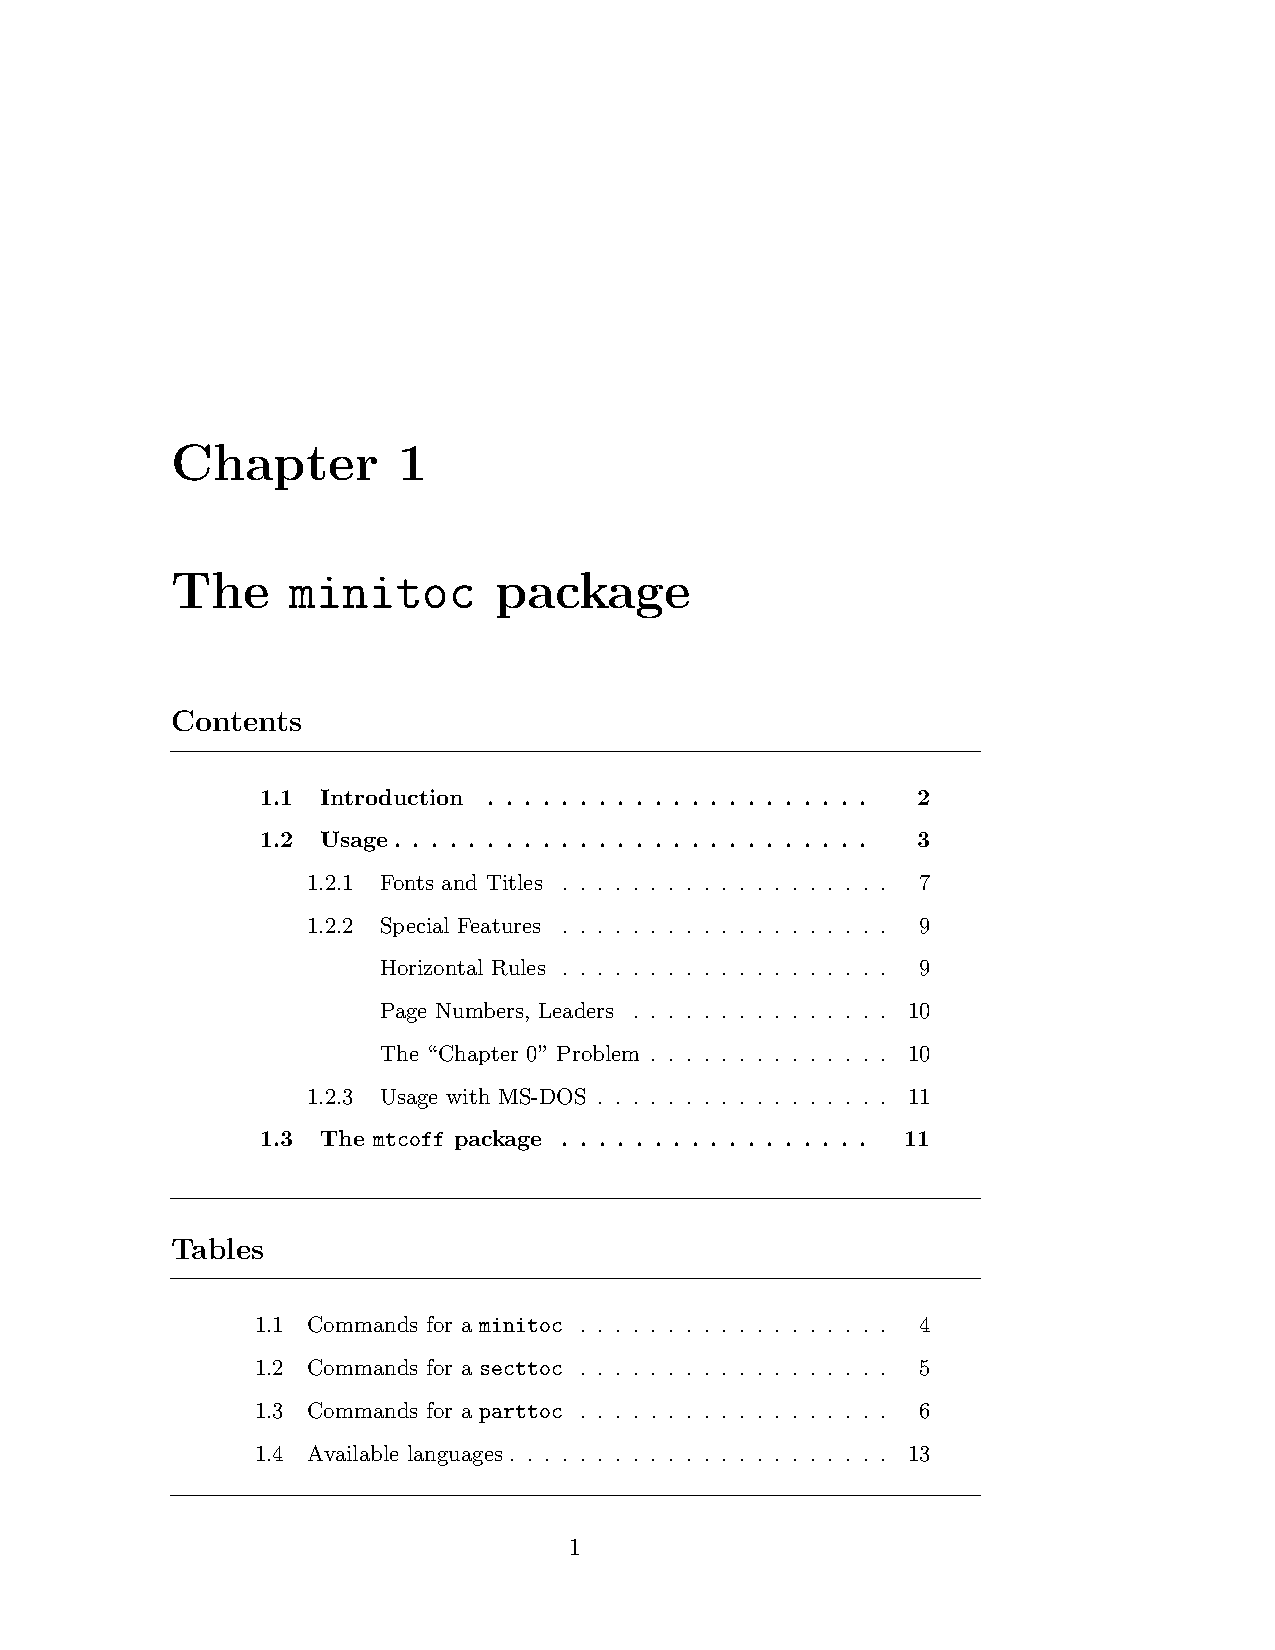
\includepdf[pages=-, fitpaper=true]{./doc/minitoc.pdf}	



% 	====================================================================================================================== chapter  찾아보기
	\chapter{찾아보기}

	% -------------------------------------- page -------------------
		\minitoc				% Creating an actual minitoc
		\doublespace
	


	% --------------------------------------- section -------------- 
	\newpage  \null
	\section{찾아보기 작성}
	
		
			

			

			

			

			

			

			

			

			

			

			







%	=========================================================================================================================================== part 편집용지의 구성
	\addtocontents{toc} {\protect\newpage}
	\part{ Page Layout}
	
			\parttoc
	%		\partlof
	%		\partlot
	
	\include{./tex/part_005}
	
	
	


% 	====================================================================================================================== chapter  면주
	\chapter{면주}


	% --------------------------------------- section --------------
	\newpage
	\section{상단면주와 하단면주}
	
	
	
	
	% --------------------------------------- section --------------
	\newpage
	\section{면주까지의 거리}
	
	
	
	% --------------------------------------- section --------------
	\newpage
	\section{면주의 범위와 괘선}
	
	
	% --------------------------------------- section --------------
	\newpage
	\section{면주의 내용}
			
			면주에 페이지번호 즉 변번호는 반드시 들어가야 한다.
	
			그리고 면번호이외에 면색인이 포함되는 경우가 많다.
	
			면주 표제에 무슨 내용을 넣어야 할 것인가?
	
			\begin{enumerate}
			\item 	책 이름이나 문서 전체의 제목은 넣지 않는 것이 좋다. \\
					왜냐하면 면주가 ‘색인’의 기능을 하고 있다 할 때 처음부터 끝까지 
					동일한 내용이 적혀 있다면 이것은 색인으로서의 기능이 없는 것이나 다름없기 때문이다.
			\item 	왼쪽면의 좀더 고정적인 것 \\
					왼쪽면에는 조금 더 고정적인 요소를 
					오른쪽면에는 조금 더 세분된 요소를 표시하는 것이 일반적이다. 
					즉 편-장 체제라면 왼쪽면에는 편표제 오른쪽면에 장표제를 싣고 
					장-절 체제라면 왼쪽면에 장표제 오른쪽면에 절표제를 싣는다.
			\item 	면번호를 판면의 바깥쪽에 찍는다. \\
					그렇게 하는 이유는 색인으로서의 면번호가 페이지를 완전히 펴지 않은 상태에서도 
					찾아볼 수 있게 하기 위함이다. \\
					안쪽에 페이지 번호를 두는 것은 좋지 않다.
			\item 	면번호와 면색인은 서로 독립적으로 취급하여도 좋다. \\
					우리나라 출판물에서 많이 취하고 있는 방법은 왼쪽면에는 왼쪽끝에 면번호를 두고 
					약간의 간격과 면색인을 적은 다음 왼쪽면의 오른쪽끝은 비우는 것이고 
					오른쪽면은 왼쪽끝을 비우고 오른쪽 끝에 면 색인과 면번호를 차례로 두는 방법이다. \\
					필요하다면 면색인을 가운데 두어도 좋겠지만 
					이것은 좌우 페이지 구분이 불필요할 때 사용할 수 있다.
			\item 	면색인의 길이는 행장의 반을 넘지 않는 것이 좋다. \\
					만약 표제행이 길다면 적당한 위치에서 줄인다.
			\end{enumerate}
	
					위의 4번은 영문 책의 경우와 관행에 차이가 있다. \\
					예컨대 라텍 표준 book 클래스의 기본값인 headings 페이지 스타일은 
					면번호를 바깥쪽에 두는 것은 동일하지만 면색인은 그 페이지의 면번호 반대편에 둔다.
	
	% --------------------------------------- section --------------
	\newpage  \null
	\section{면주의 서체와 크기}
	
	
	% --------------------------------------- section --------------
	\newpage  \null
	\section{면주와 면번호 붙이기}


% --------------------------------------- section -------------- 주석문
\newpage \null
\section{주석문}



	% -------------------------------------- page -------------------
	\newpage  \null
	\section{페이지 구성 예}
	
		\singlespacing
		\setlength{\fboxsep}{12pt}
		\begin{boxedminipage}[c]{1.0\linewidth}
			\begin{verbatim}
				% --------------------------------- 페이지 스타일 지정
				\usepackage{fancyhdr}
				\pagestyle{fancy}
				
				\fancyhead{} % clear all fields
				\fancyhead[LO]{\small \leftmark}
				\fancyhead[RE]{\small \leftmark}
				
				\fancyfoot{} % clear all fields
				\fancyfoot[LE,RO]{\large \thepage}
				%\fancyfoot[CO,CE]{\empty}
				
				\renewcommand{\headrulewidth}{0.4pt}
				\renewcommand{\footrulewidth}{0.4pt}
			\end{verbatim} 
		\end{boxedminipage}
		\doublespacing
	
	




		
% 	====================================================================================================================== chapter  페이지 형식
	\chapter{페이지 형식}

	% -------------------------------------- page -------------------
		\minitoc				% Creating an actual minitoc

	% --------------------------------------- section --------------
	\newpage  \null
	\section{다단 편집}
	\null
	
			\begin{itemize}
			\item one column
			\item two column
			\end{itemize}
	
	% --------------------------------------- section --------------
	\newpage  \null
	\section{양면 인쇄}
	\null
	
			\begin{itemize}
			\item one side
			\item two side
			\end{itemize}

	% --------------------------------------- section --------------
	\newpage  \null
	\section{첫페이지 위치}
	\null
	
			\begin{itemize}
			\item open any
			\item open right
			\end{itemize}
	
	% --------------------------------------- section --------------
	\newpage  \null
	\section{표지 인쇄}
	\null
	
			\begin{itemize}
			\item no title page
			\item title page
			\end{itemize}























			
			
% 	====================================================================================================================== chapter  본문 작성
	\chapter{본문 작성}
					
	% -------------------------------------- page -------------------
		\minitoc				% Creating an actual minitoc
		\doublespace




					
	% --------------------------------------- section -------------- 
	\newpage
	\section{장, 절의 설정}
					

		장, 절을 작성하기 위한 명령어는 다음과 같다.\\
		단 \verb|\chapter|명령어는 ariticle 클래스에서 사용할 수 없다.\\
		일반적으로 논문에서는 소소절(\verb|\subsubsection|)까지 쓴다.\\

		\verb|\part [목차에 나타날 부 제목] {부 제목 }|\\
		\verb|\chapter [목차에 나타날 부 제목] {부 제목 }|\\
		\verb|\section [목차에 나타날 부 제목] {부 제목 }|\\
		\verb|\subsection [목차에 나타날 부 제목] {부 제목 }|\\
		\verb|\subsubsection [목차에 나타날 부 제목] {부 제목 }|\\
		\verb|\paragraph [목차에 나타날 부 제목] {부 제목 }|\\
		\verb|\subparagraph [목차에 나타날 부 제목] {부 제목 }|\\


	% --------------------------------------- section -------------- 
	\newpage
	\section{목차에서의 장, 절의 표시}


		\subsection{목차에서의 장, 절의 표시}

			\verb|\setcounter{tocdepth}{3}|\\



		\subsection{본문에서의 장, 절의 표시}

			\verb|\setcounter{secnumdepth}{3}|\\
	
	
			\begin{table}[hbp]
			\caption{장, 절 수준 및 번호}
			\centering 

%			\begin{tabular}{ p{0.2\textwidth} p{0.2\textwidth} p{0.2\textwidth} }
%			\toprule
%			부 		&(part)			& -1\\
%			장 		&(chapter)		& 0\\
%			절 		&(section)		& 0\\
%			소절 	&(subsection)	& 0\\
%			소소절 	&subsubsection)	& 0\\
%			문단 	&(paragraph)	& 0\\
%			소문단 	&(subpargraph)	& 0\\
%			\bottomrule
%			\end{tabular} 

			\end{table}

		\newpage  \null
		\subsection{장, 절  번호의  표시 제어}
	
			또 숫자를 붙이고 싶지 않지만, 장이나 절 처럼 사용하고 싶다면 *를 붙이면 된다.\\

			\verb|\chapter*{ 장 제목}|\\

			이 명령어는 다른 경우, 예를 들어 수식에도 똑같이 작용될수 있다.\\

			\verb|\section*{}}| 을 이용하면 section number가 사라진다.		
			하지만 subsection과 이후 section에 까지 numbering 에 영향을 미치므로, 
			그냥 section number를 숨기고 싶은 의도라면 \verb|\addtocounter{section}{1}| 를 
			한줄 추가해주면 된다.

			결론 :\\
			\verb|\section*{Problem 1}|\\
			\verb|{\addtocounter{section}{1}|


	% --------------------------------------- section -------------- 
	\newpage
	\section{chapter and section}



	% --------------------------------------- section -------------- 
	\newpage 
	\section{Customize chapters and sections}


		당신은 titlesec package를 사용하여 
		쉽게 장, 절 및 하위 섹션 스타일의 사용자 정의를 할 수 있다.\\
		
		\setlength{\fboxsep}{12pt}
		\begin{boxedminipage}[c]{1.0\linewidth}
		\small  \singlespace
		\begin{verbatim}
\documentclass[a4paper,12pt]{book}
\usepackage{titlesec}
 
\titleformat  {\chapter} % command
              [display]    % shape
              {\bfseries\Large\itshape} % format
              {Story No. \ \thechapter} % label
              {0.5ex} % sep
              {   \rule{\textwidth}{1pt}
                   \vspace{1ex}
                   \centering
              } % before-code
              [  \vspace{-0.5ex}%
                  \rule{\textwidth}{0.3pt}
              ] % after-code
 
\titleformat  {\section}[wrap]
              {\normalfont\bfseries}
              {\thesection.}{0.5em}{}
 
\titlespacing{\section}{12pc}{1.5ex plus .1ex minus .2ex}{1pc}

\begin{document}
  \chapter{Let's begin}
     \section{First Attempt}
                  Lorem ipsum dolor sit amet, 
    \section{Second attempt}
                  Lorem ipsum dolor sit amet, 
 \end{document}
		\end{verbatim}
		\end{boxedminipage}
		\doublespace \normalsize


		\newpage   \null
	% -------------------------------------- page -------------------
		\subsection{title format }

		\setlength{\fboxsep}{12pt}
		\begin{boxedminipage}[c]{1.0\linewidth}
		\small  \singlespace
		\begin{verbatim}
\titleformat{<command>}
            [<shape>]
           {<format>}
           {<label>}
           {<sep>}
           {<before-code>}
           [<after-code>]
		\end{verbatim}
		\end{boxedminipage}
		\doublespace \normalsize

		\begin{itemize}[itemsep=0.0em]
		\item	$<$command$>$는 명령을 재정의 하는것이다.\\
				\verb|\part, \chapter, \section, \subsection, \subsubsection,|
				\verb|\paragraph| or \verb|\subparagraph.|
		\item	$<$shape$>$는 단락 모양을 정의 한다.\\
				possible values are: hang, block, display, runin, leftmargin, rightmargin, drop, wrap, frame.
		\item	$<$forma$>$
				$<$forma$>$은 형식을 적용한다.\\
				for example \verb|\normalfont\Large\bfseries|\\
				font : rm sf tt md bf up it sl sc\\
				size : big medium small tiny\\
				align : raggedleft center raggedright
		\item	$<$label$>$ specify sectioning label.
		\item	$<$sep$>$\\
				$<$sep$>$ is the horizontal separation between label and title body \\
				and it must be a length and not be empty.
		\item	$<$before-code$>$is code preceding the title body.
		\item	$<$after-code$>$ is code following the title body.
		\end{itemize}


		\newpage   \null
	% -------------------------------------- page -------------------
		\subsection{title format - shape}


			\begin{itemize}[itemsep=0.0em]
			\item	hang\\
					hang is the default value, with a hanging label. (Like the standard \verb|\section|.)
			\item	block\\
					블록은 추가 서식없이 블록(단락)의 전체 제목을 식자. 
					중심 타이틀과 특별한 ormatting에 유용한
					(사진, pspicture 등과 같은 그래픽 도구를 포함)
			\item	display\\
					display는 별도의 단락에 라벨을 넣습니다\\
					 (Like the standard \verb|\chapter|.)
			\item	runin\\
					runin은 삽입된 타이틀이다 \\
					(Like the standard \verb|\paragraph|.)
			\item	leftmargin\\
					leftmargin는 왼쪽 여백에서 제목을 넣습니다.
					페이지의 맨 마지막에 있는 제목은 다음 단계로 이동합니다.
					큰 제목 underfull 페이지로 이어질 수 있음을 의미 아래쪽 여백에 돌출되지 않습니다.\\
					이 경우에는 사용자가 페이지 요소의 신축성을 증가시킬 수있다,.
					\verb|\raggedbottom|를 사용하거나 후술하는 패키지 nobottomtitles 옵션을 사용한다.\\
					사용 된기구는 마진 동위와는 독립적이기 때문에, 그들은 겹칠 수있다. 
					사용되지 않는 동의어는 여백입니다.
			\item	rightmargin\\
					rightmargin is like leftmargin but at the right margin.
			\item	drop\\
					drop wraps the text around the title, provided the first paragraph is longer than the title (if not, they overlap). 
					The comments in leftmargin also apply here.
			\item	wrap\\
					wrap is quite similar to drop. 
					The only difference is while the space reserved in drop for the title is fixed, in wrap is automatically readjusted to the longest line. The limitations explained below related to calcwidth also apply here.
			\item	frame\\
					frame Similar to display, but the title will be framed
			\end{itemize}



		\newpage   \null
	% -------------------------------------- page -------------------
		\subsection{title spacing }

		\setlength{\fboxsep}{12pt}
		\begin{boxedminipage}[c]{1.0\linewidth}
		\small  \singlespace
		\begin{verbatim}
 \titlespacing{<command>}
          {<left>}
          {<before-sep>}
          {<after-sep>}
		\end{verbatim}
		\end{boxedminipage}
		\doublespace \normalsize\\


		\begin{itemize}[itemsep=0.0em]
		\item	$<$left$>$ increases the left margin.
		\item	$<$before-sep$>$ is the vertical space before the title.
		\item	$<$after-sep$>$ is the separation between title and non-sectioning text.
		\end{itemize}


	% --------------------------------------- section -------------- 
	\newpage 
	\section{chapters and sections 번호 }

		\setlength{\fboxsep}{12pt}
		\begin{boxedminipage}[c]{1.0\linewidth}
		\small  \singlespace
		\begin{verbatim}
\documentclass{article}
\usepackage{titlesec}
\setcounter{secnumdepth}{4}

\titleformat{\paragraph}  # 명령
           {\normalfont\normalsize\bfseries}  % 형태
           {\theparagraph}{1em}{}                 % 라벨

\titlespacing*{\paragraph}
           {0pt}
           {3.25ex plus 1ex minus .2ex}
           {1.5ex plus .2ex}

\begin{document}

\section{Test Section} test
\subsection{Test Subsection} test
\subsubsection{Test Subsubsection} test
\paragraph{Test Modified Paragraph} test

\end{document}
		\end{verbatim}
		\end{boxedminipage}
		\doublespace \normalsize\\


	% --------------------------------------- section -------------- 
	\newpage  \null
	\section{본문}



	% --------------------------------------- section -------------- 
	\newpage  \null
	\section{각주}


		\setlength{\fboxsep}{12pt}
		\begin{boxedminipage}[c]{1.0\linewidth}
			\verb|\footnote {각주 내용 }|
		\end{boxedminipage}




	% --------------------------------------- section -------------- 
	\newpage  \null
	\section{난외주}

		\setlength{\fboxsep}{12pt}
		\begin{boxedminipage}[c]{1.0\linewidth}
			\verb|\marginpar {난외주 내용}|
		\end{boxedminipage}




	% --------------------------------------- section -------------- 
	\newpage  \null
	\section{인용}

		\setlength{\fboxsep}{12pt}
		\begin{boxedminipage}[c]{1.0\linewidth}
			\verb|\begin { quote }|\\
			( 인용문 내용 )\\
			\verb|\end { quote }|
		\end{boxedminipage}



	% --------------------------------------- section -------------- 
	\newpage  \null
	\section{참고문헌, 표, 그림 넣기}


	% --------------------------------------- section -------------- 
	\newpage  \null
	\section{상호 참조}


	% --------------------------------------- section -------------- 
	\newpage  \null
	\section{프로그램 코드를 그대로 입력하기}

		\setlength{\fboxsep}{12pt}
		\begin{boxedminipage}[c]{1.0\linewidth}
			\verb|\begin { verbatim }|\\
			( 인용문 내용 )\\
			\verb|\end { verbatim }|
		\end{boxedminipage}


	% --------------------------------------- section -------------- 
	\newpage  \null
	\section{각 장을 파일로 나누기}




					

					

% ===========================================================	part		=============
		\addtocontents{toc}{\protect\newpage}
		\part{List - 개조식 문서 작성}

		\parttoc
	%	\partlof
	%	\partlot


		\include{./tex/Part_000_list}




%	================================================================================================================================= part 글자모양
	\addtocontents{toc} {\protect\newpage}
	
			\part{글자 모양}
			
			\parttoc
	%		\partlof
	%		\partlot



		


%	---------------------------------------------------------------------------------------------------
%
%	\part{글자 모양}
%
%	---------------------------------------------------------------------------------------------------







% ========================================== chapter ============
\newpage  
\chapter{글꼴 크기}

	% -------------------------------------- page -------------------
		\minitoc				% Creating an actual minitoc

		
	% --------------- subsection -------------- 글꼴 크기 조정
	\clearpage
	\section{글꼴 크기 조정}
	\null
	
	
		위드프로세서에서는 폰트의 크기를 조정함으로써 글자 크기를 조정했지만 \LaTeX에서는
		문서의 기본 글꼴 크기가 정해져 있고, 이에 비례하여 글자 크기를 조정한다.
		
		
			\begin{table}[hbp]
			\caption{글자 크기}
			\centering
			\begin{tabular}{l  l  l }
			\toprule
			명령어 & 결과 \\
			\toprule
			\verb|\tiny|				& \tiny결과 &\normalsize{결과}\\
			\verb|\script size|		& \scriptsize{결과} \\
			\verb|\foot notee size| 	& \footnotesize{결과} \\
			\verb|\small|			& \small{결과} \\
			\verb|\normal size| 		& \normalsize{결과} \\
			\verb|\large| 			& \large{결과} \\
			\verb|\Large| 			& \Large{결과} \\
			\verb|\LARGE| 			& \LARGE{결과} \\
			\verb|\huge| 			& \huge{결과} \\
			\verb|\Huge| 			& \Huge{결과} \\
			\bottomrule
			\end{tabular}%
			\end{table}%
			
			
			
			
		
				
	% --------------- subsection --------------
	\clearpage
	\section{큰 글꼴 사용 : ext size package }
	\null
	
		\subsection*{큰 글꼴 사용}
	
			표준 크기 (10,11pt)가 충분하지 않다면, extsizes 패키지를 이용하면 된다.\\
			
			\begin{boxedminipage}[c]{1.0\linewidth}
			\begin{verbatim}
				\documentclass[17pt]{ext article}
			\end{verbatim}
			\end{boxedminipage}
			
			문서의 기본 글꼴 크기를 바꾸려면 위 명령어를 프리엠블에 쓴다. 
			\\\\
			이 패키지는 확장된 표준 문서 클래스 옵션을 제공하여 8,9,10,11,12,14,17,20 포인트 문서를 
			작성할 수있도록 해준다.
		
	% --------------- subsection --------------
	\clearpage
	\section{큰 글꼴 사용 : fix-cm package }
	\null
	
			LaTeX은 글자 크기를 tiny, scriptsize, footnotesize, small, normalsize, 
			large, Large, LARGE, huge, Huge 명령을 이용해서 정합니다.
			nomalsize의 크기가 정해지면 그에 맞게 다른 크기가 변합니다.
			그런데, 가장 큰 Huge라 해도 그리 크지가 않습니다. 
			만약 문서의 표지 제목 등 큰 글자가 필요할 때는 어떻게 할까요? 
			여러가지 방법이 있지만 fontsize 명령을 사용하는 게 제일 편합니다.\\
			
			\singlespace
			\begin{boxedminipage}[c]{1.0\linewidth}
				\begin{verbatim}
					\usepackage{fix-cm}
					...
					\fontsize{<font size>}{<baselineskip>}
				\end{verbatim}
			\end{boxedminipage}\\

			간단한 예는 다음과 같습니다.\\
			
			\begin{boxedminipage}[c]{1.0\linewidth}
				\begin{verbatim}
					\documentclass[a4paper]{article}
					\usepackage{kotex}
					\usepackage{fix-cm}
					\begin{document}
					\fontsize{80}{70} \rmfamily 큰 글자 A
					\end{document}
				\end{verbatim}
			\end{boxedminipage}\\
			\doublespace
			
			빨간색의 코드를 넣어야 영어 글자가 제대로 커집니다. 결과는 다음과 같습니다.		\\
			{\Huge Huge size 큰 글자 A}\\
			{\fontsize{70}{70} \rmfamily 70 size 큰 글자 A}
					
			\newpage
			{\fontsize{20}{20}  \rmfamily 20 point \par}
			큰 글자 A \par
			{\fontsize{30}{35} \rmfamily 큰 글자 A \par}
			큰 글자 A \par
			{\fontsize{30}{35} \selectfont 큰 글자 A Big\\ More \par}	
			큰 글자 A \par
			\doublespace
																														\subsection*{사용시 주의 사항}
																														반드시\{ \} 사용하여 범위를 제한 할것
																																
																																		
																																				
% ========================================== chapter ============
\newpage  
\chapter{글꼴 모양}


% ========================================== chapter ============
\newpage  
\chapter{글자 색}

	

% ========================================== chapter ============
\newpage  
\chapter{윗첨자, 아래첨자}

																																						
																																								
																																										
																																												
							








% ========================================== chapter ============
\newpage  
\chapter{글꼴}

	% ------------------------------------------ section ------------ 
	\newpage  \null
	\section{글꼴}

			ko.TeX에서 기본 자원하는 기본 글꼴 목록 표\ref{gibonFont} 과 
			기본 설정은 표\ref{gibonSetting}와 같다. 
			확장글꼴과 트루타입글꼴의 추가와 같이 더 자세한 사항은 ko.TeX 가이드 문서를 참조하라.
		
	\subsection{기본 글꼴}
				\vspace{-1cm}
				\begin{table}[hbp]
				\caption{ko.TeX기본 글꼴 목록}
				\centering
				\begin{tabular}{c c}
				\toprule
				글꼴 & 글꼴 이름\\
				\toprule
				명조	& utbt  \\
				고딕	& utgt \\
				타자	& uttz \\
				그래픽	& utgr \\
				\bottomrule
				\end{tabular}%
				\label{gibonFont}%
				\end{table}%
		
	\subsection{기본 설정}
				\vspace{-1cm}
				\begin{table}[hbp]
				\caption{ko.TeX 문서 한글 기본 설정}
				\centering
				\begin{tabular}{c c c c c}
				\toprule
				언어 종류 & rm 글꼴 이름 & sf 글꼴 이음 & tt 글꼴 이음 & emph 글꼴 이음 \\
				\toprule
				한글 & utbt & utgt & uttz & utgr \\
				한자 & utgt & utgt & uttz & utgr \\
				\bottomrule
				\end{tabular}%
				\label{gibonSetting}%
				\end{table}%

	% ------------------------------------------ section ------------ 
	\newpage  \null
	\section{글꼴}




			몇 가지 생각나는 대로 말씀드리면 다음과 같습니다. 
			우선, LaTeX은 "특정 폰트"에 대해서 무관심하다고 말할 수 있습니다. 
			LaTeX이 유지하고자 하는 것은 문서의 논리적 일관성이지 
			외형상의 모양이 아니므로(그것이 중요하지 않다는 뜻은 아닙니다), 
			
			LaTeX으로 문서를 작성했을 때, 그것이 결과적으로 어떤 폰트로 식자될 것인가는 최
			종적인 편집자가 결정할 문제이지 문서 작성자가 신경쓸 일이 아니라고 생각한다고 
			볼 수 있습니다.
			
			그러므로, LaTeX에서는 
			이를테면, "세리프 글꼴", "산세리프 글꼴", "타이프라이터 글꼴"이라는 
			세 가지 기본적인 폰트를 하나의 문서에서 사용하는 것으로 일단 상정합니다. 
			각각 한글폰트로는 명조체, 고딕체, 타자체 정도에 해당하는 것이 아닌가 싶습니다만, 
			1:1 대응이 되는지는 잘 모르겠습니다. 
			이 세 가지를 각각 rm, sf, tt라고  부르고 "글꼴 가족"(font family)이라고 합니다.
			 주1. 이 이외의 글꼴 가족을 더 정의해서 쓰는 것은 물론 가능합니다.
			
			각각의 글꼴 가족에 대해서 
			모양(shape)과 계열(series)이라는 추가적인 옵션이 있습니다. 
			모양에는 itshape(이탤릭), slshape(기울인 모양), upshape(곧게선 모양), 
			scshape(작은대문자모양) 등이 있고, 
			계열에는 mdseries(보통글꼴 계열), bfseries(굵은 계열), extended(늘린 계열), 
			condensed(줄인 계열) 등이 있습니다.\\
			
			\textbf{모양(shape)}\\
			\begin{itemize}[topsep=-1.0em, itemsep=-0.5em]
			\item	itshape	(이탤릭)
			\item	slshape	(기울인 모양)
			\item	upshape	(곧게선 모양)
			\item	scshape	(작은대문자모양)
			\end{itemize}
			
			
			\paragraph*{계열(series)}
			\begin{itemize}[topsep=-1.0em, itemsep=-0.5em]
			\item	mdseries	(보통글꼴 계열)
			\item	bfseries		(굵은 계열)
			\item	extended	(늘린 계열)
			\item	condensed	(줄인 계열)
			\end{itemize}
			
			 
			LaTeX은 이 명령들을 결합해서 폰트를 지정합니다. 
			예를 들면, \verb|\bfseries|라고 하면, 
			현재의 폰트 모양에서 계열만을 bfseries로 바꾸라는 뜻입니다. 
			이 선언은 한번 바뀌면 이후로도 계속 영향을 미치기 때문에, 
			\verb|\textbf{ABCDEFghi}|와 같은 식으로 일부에 대해서만 적용하도록 하는 
			\verb|\text...| 명령이 존재합니다.
			
			아무런 지정도 하지 않은 상태에서는 \verb|\normalfont|가 적용되는데, 
			일반적으로 serif, upshape, mdseries가 기본 글꼴입니다. \\
			
			이제 이것을 특정 폰트와 결합해야 합니다. TeX/LaTeX은 시스템의 폰트를 이용하지 
			않습니다. 사실, 엄격히 말하자면 LaTeX이 할 수 있는 일은, 최종 출력기에게 "어떠
			어떠한 폰트를 사용해서 이 글자를 어느 위치에 식자하라"는 명령만을 할 수 있을 뿐
			이고, 폰트 자체를 사용하지 않습니다.\\
			
			 주2. TeX의 출력포맷인 .dvi에는 폰트에 대한 "정보"만이 들어 있고 폰트는 들어 있
			지 않습니다.\\
			
			TeX이 식자에 사용하는 정보는 .tfm이라는 Font Metric 파일에 있습니다. 
			다시 말하면 .tfm만을 TeX이 이해한다고 할 수 있지요. 
			말씀하신 Arial이나 Times New Roman 같은 것은 .tfm 형태로 존재하지 않는 한 
			TeX이 사용할 수 없습니다.
			
			TeX이 기본으로 제공하는 영문폰트는 TeX의 창시자인 D. Knuth가 디자인한 Computer 
			Modern이라는 글꼴 계열입니다.
			이 글꼴은 예컨대, 다음과 같은 방법으로 이 폰트를 결합시킵니다.\\
			
			\verb|\rmfamily| => Computer Modern Roman\\
			\verb|\sffamily| => Computer Modern Sans Serif\\
			\verb|\ttfamily| => Computer Modern Typewriter\\
						
			같은 Computer Modern Roman 글꼴이라 해도, 각각의 shape와 series에 따라서 (심지
			어 글꼴 크기에 따라서도) 별도의 .tfm이 준비되어 있습니다.
			
			---
			LaTeX의 발달에 따라서 다른 폰트도 문서에 사용할 수 있게 하려는 노력이 있었습니
			다. 
			예를 들면 범용의 35개의 LaserWriter Postscript Font를 쓸 수 없는가? 이를 위
			해서 각각의 글꼴 가족에 cm이 아닌 다른 폰트를 대응시켜 사용할 수 있습니다.\\
			
			우리는 일반적으로 Times라고 쉽게 말하지만, 사실 Adobe Times는 아무나 사용할 수 
			있는 공개 글꼴이 아니고 저작권이 존재하는 상업용 글꼴입니다. 이 Times를 흉내낸 
			(가짜) times를 자유롭게 사용할 수 있을 뿐인데, 대표적인 것은 GhostScript와 함
			께 제공되는 urw 폰트입니다. (윈도 시스템은 그 나름대로 글꼴을 라이센싱해서 제공
			하므로, 사용할 수 있는 글꼴의 형태와 폭이 또 다르다고 할 수 있습니다.)
			이 urw times를 Computer Modern Roman 대신 사용하려면 약간 복잡한 절차를 거쳐서 
			urw times의 .tfm을 정의한 다음, \verb|\rmfamily|를 부르는 곳에서 해당 .tfm을 연결시켜
			주면 될 것입니다. 다행히 주요 Postscript 영문 글꼴에 대해서는 이런 작업이 TeX 
			Implementation에서 다 되어 있고, 사용자는 단순히 다음과 같이 한 줄을 .tex 파일
			의 preamble에 적어주면 됩니다.
			

			\verb|\usepackage{times}|

			그런데, 이것은 오로지 본문 글꼴만 바꾸는데, 수학 글꼴(TeX은 수학식에는 본문 폰
			트와는 별도의 폰트를 적용합니다.)에도 times 비슷한 폰트를 쓰도록 하려는 목적에
			서 요즘은
			
			\verb|\usepackage{mathptmx}|
			
			이런 식으로 할 것을 권장합니다.
			
			아무튼, (오래된 패키지라는 사람도 있지만) \verb|\usepackage{times}|하면, 
			\verb|\sffamily|에는 helvetica 폰트를 선택해줍니다.
			이밖에 times를 본문으로 하고 helvetica나 다른 sansserif(물론 공개 글꼴 중에서)
			를 선택하게 해주는 스타일 패키지 중에, 사용이 간편하고 품위도 나쁘지 않은 것으
			로는 txfonts라는 것이 있습니다\\. 
			
			\verb|\usepackage{txfonts}|\\
			
			이 스타일을 얹으면 rm에는 times와 비슷한 글꼴을, sf에는 helvetica 비슷하지만 크
			기가 helvet보다 조금 더 적절하고 모양도 다듬어진 글꼴을 사용할 수 있게 됩니다. 
			
			---
			마지막으로, Arial과 Times New Roman을 "반드시" 써야 하고, TeX이 기본적으로 제공
			하는 폰트에 불만이시라면, 이것은 (La)TeX의 폰트 선택 스킴을 공부하셔서 .tfm을 
			추출하고 스타일을 정의해서 쓰셔야 할 것입니다. 
			윈도 기본 폰트에 대해서는 이미 이런 작업을 해두신 분들이 아마도 있을 것입니다만, 
			TeX 배포판에 기본적으로 포함되어 있지는 않을 것으로 생각합니다.
			
			---
			더 쉽게 재미있게 설명해주실 분을 기대합니다.













































	% ------------------------------------------ section ------------ 
	\newpage  \null
	\section{글꼴 바꾸기}

			하나의 문서에 글꼴이 많이 쓰이면 쓰일수록 통일성이 떨어지고, 
			한눈에 읽기도 좋지 않다. 그러므로 되도록 글꼴을 유지할 것을 권한다.
			그럼에도 표준 글꼴이 마음에 들지 않는다면 다음의 명령어를 사용할 수 있다.
			\begin{framed}
			\verb|\SetHangulFonts{rm(roma)}{ss(san serif)}{tt(typewriter)}|
			\verb|\SetHanjaFonts{rm(roma)}{ss(san serif)}{tt(typewriter)}|
			\end{framed}
			위의 명령은 각각 한글과 한자 글꼴을 지정한다. 
		
			
	

	% --------------- subsection -------------- 글꼴 모양
	\clearpage  \null
	\section{글꼴 모양}
	
		기본적인 형식은 아래와 같으며, 한글의 경우 이탤릭체보다는 굵은 글씨를 쓰는 경우가 많다.
		
	
			\begin{table}[hbp]
			\caption{글자 모양}
			\centering
			\begin{tabular}{c c c}
			\toprule
			명령어 & 환경 & 결과 \\
			\toprule
			\verb|\textnormal|	& textnormal 	& 결과 \\
			\verb|\textit|		& itshape		& \Large\textit{결과} \\
			\verb|\emph| 		& 없음			& \Large\emph{결과} \\
			\verb|\textbf|		& bfseries	 	& \Large\textbf{결과} \\
			\verb|\underline| 	& underline 		& \Large\underline{결과} \\
			\bottomrule
			\end{tabular}%
			\end{table}%
	
	
			\begin{table}[hbp]
			\caption{글자 모양}
			\centering
			\begin{tabular}{c c c}
			\toprule
			명령어 & 환경 & 결과 \\
			\toprule
			\verb|\rm|	& Roman 	& \rm{결과 result} \\
			\verb|\sl|	& Slanted	& \sl{결과 result} \\
			\verb|\it| 	& Italic		& \it{결과 result} \\
			\verb|\tt|	& Typewrite	& \tt{결과 result} \\
			\verb|\bf| 	& Bold 		& \bf{결과 result} \\
			\bottomrule
			\end{tabular}%
			\end{table}%

	
		
	% --------------- subsection -------------- 밑줄 긋기
	\clearpage \null
	\section{밑줄 긋기}
	
		보통 밑줄을 사용하지 않는다. 혹 사용한다 하더라도 \verb|\underline|으로 충분하다. 
		그래도 꼭 다양한 밑줄을 그어야 한다면 ulem 패키지를 사용하면 된다.





















% 	====================================================================================================================== chapter  특수문자
	\newpage
	\chapter{특수문자}
	
	% -------------------------------------- page -------------------
		\minitoc				% Creating an actual minitoc
	

		
%
%		\usepackage{pifont}		% 		
%		\usepackage{textcomp}		%	 		
%		\usepackage{gensymb}		% 		
%		\usepackage{marvosym}		% 		


% ========================================== chapter ============
	\chapter{특수문자}

	% -------------------------------------- page -------------------
	%	\nomtcrule         		% removes rules = horizontal lines
	%	\nomtcpagenumbers  % remove page numbers from minitocs
		\newpage
		\minitoc				% Creating an actual minitoc
	%	\doublespace



% ------------------------------------------ section ------------ 특수문자
	\section{특수 문자}

		\subsection{따옴표}
			타지기에서처럼 $''$를 사용해서는 안된다. 
			
			출판물에서는 특별한 여는 따옴표와 닫는 따옴표를 사용한다. 
			\LaTeX에서는 두개의 $'$ (grave accent)와 두개의 $'$(vertical quote)를 
			각각 여는 따옴표와 닫는 따옴표로 사용한다.
			작은 따옴표의 경우에는 각각의 기호를 한 번씩만 사용하면 된다.
		
			\begin{quote}
			(ㄱ)왼쪽 따옴표 (ㄱ)오른쪽 따옴표
			\end{quote}
		
			\paragraph{여는 따옴표}
			여는 따옴표는 표준 자판 제일 윗쪽의 제일 왼쪽 키에 할당되어 있는 문자
			(back-tick 혹은 grave accent)를 사용한다.
		
			\paragraph{닫는 따옴표}
			닫는 따옴표는 자판 가운데줄 오른쪽 끝에 있는 작은 따옴표 문자(vertical quote)를 사용한다.
		
		
		\subsection{대시와 히이픈}
				
						
		\subsection{틸데(\~{})}
	
		\subsection{도 기호($^{\circ}$)}
	
			\begin{framed}
			\verb|$30\,^{\circ} \mathrm{C} $|  	$30\,^{\circ} \mathrm{C} $ \\
			\verb|$30^{\circ} \mathrm{C} $|  		$30^{\circ} \mathrm{C} $
			\end{framed}
	
		\subsection{유로 통화 기호}
		
	
		\subsection{줄임표}




% ------------------------------------------ section ------------ 
	\section{특수문자}


	% --------------------------------------------------
	\subsection{ textcircled }
	\begin{itemize}[itemsep=-0.5em,leftmargin=4em]
	\item[	\textcircled {\footnotesize A} ] \textbackslash textcircled \{\textbackslash footnotesize A\}
	\item[	\textcircled {\footnotesize B} ] \textbackslash textcircled \{\textbackslash footnotesize B\}
	\item[	\textcircled {\footnotesize C} ] \textbackslash textcircled \{\textbackslash footnotesize C\}
	\item[	\textcircled {\footnotesize D} ] \textbackslash textcircled \{\textbackslash footnotesize D\}
	\item[	\textcircled {\footnotesize E} ] \textbackslash textcircled \{\textbackslash footnotesize E\}
	\item[	\textcircled {\footnotesize F} ] \textbackslash textcircled \{\textbackslash footnotesize F\}
	\item[	\textcircled {\footnotesize G} ] \textbackslash textcircled \{\textbackslash footnotesize G\}


	\item[	\textcircled {\footnotesize 1} ] \textbackslash textcircled \{\textbackslash footnotesize 1\}
	\item[	\textcircled {\footnotesize 2} ] \textbackslash textcircled \{\textbackslash footnotesize 2\}
	\item[	\textcircled {\footnotesize 3} ] \textbackslash textcircled \{\textbackslash footnotesize 3\}

	\item[	\textcircled {\footnotesize 11}] \textbackslash textcircled \{\textbackslash footnotesize 11\}
	\item[	\textcircled {\scriptsize   11}] \textbackslash textcircled \{\textbackslash scriptsize   11\}
	\item[	\textcircled {\tiny         11}] \textbackslash textcircled \{\textbackslash tiny         11\}


	\item[	\textcircled {\footnotesize 가}] \textbackslash textcircled \{\textbackslash footnotesize 가\}
	\item[	\textcircled {\scriptsize   가}] \textbackslash textcircled \{\textbackslash scriptsize   가\}
	\item[	\textcircled {\tiny         가}] \textbackslash textcircled \{\textbackslash tiny         가\}

	\end{itemize}

	% --------------------------------------------------
	\subsection{gensymb}

	\celsius \\
	\perthousand \\
	\degree	\\

	\textbullet ~ textbullet

	\textzerooldstyle\\

	$\div$\\

	% --------------------------------------------------
	\subsection{textcomp}

			\verb|\usepackage{textcomp}|
			

	\begin{itemize}
		\item	\textcelsius  		\verb|\textcelsius|
		\item	\textpertenthousand	\verb|\textpertenthousand|
		\item	\textperthousand		\verb|\textperthousand|
		\item	\textreferencemark		\verb|\textreferencemark|
	\end{itemize}





	\newpage \null
	\subsection{Table 211: marvosym Engineering Symbols}

			\verb|\usepackage{marvosym}|


	\begin{itemize}
		\item	\Beam		\verb|	\Beam	|
		\item	\Force		\verb|	\Force	|
		\item	\Octosteel		\verb|	\Octosteel	|
		\item	\RoundedTTsteel		\verb|	\RoundedTTsteel	|
		\item	\Bearing		\verb|	\Bearing	|
		\item	\Hexasteel		\verb|	\Hexasteel	|
		\item	\Rectpipe		\verb|	\Rectpipe	|
		\item	\Squarepipe		\verb|	\Squarepipe	|
		\item	\Circpipe		\verb|	\Circpipe	|
		\item	\Lefttorque		\verb|	\Lefttorque	|
		\item	\Rectsteel		\verb|	\Rectsteel	|
		\item	\Squaresteel•		\verb|	\Squaresteel•	|
		\item	\Circsteel		\verb|	\Circsteel	|
		\item	\Lineload		\verb|	\Lineload	|
		\item	\Righttorque		\verb|	\Righttorque	|
		\item	\Tsteel		\verb|	\Tsteel	|
		\item	\Fixedbearing		\verb|	\Fixedbearing	|
		\item	\Loosebearing		\verb|	\Loosebearing	|
		\item	\RoundedLsteel		\verb|	\RoundedLsteel	|
		\item	\TTsteel		\verb|	\TTsteel	|
		\item	\Flatsteel		\verb|	\Flatsteel	|
		\item	\Lsteel		\verb|	\Lsteel	|
		\item	\RoundedTsteel		\verb|	\RoundedTsteel	|
	\end{itemize}




%	\subsection{\asterisus asterisus}











					



%	=========================================================================================================================================== part 문서 편집
	\addtocontents{toc} {\protect\newpage}
	
			\part{문서 편집}
			\parttoc
	%		\partlof
	%		\partlot
	


% 	====================================================================================================================== chapter  입력
	\newpage
	\chapter{입력}

	% -------------------------------------- page -------------------
		\minitoc				% Creating an actual minitoc




% 	====================================================================================================================== chapter  문단 모양
	\chapter{문단모양}
	\newpage


		% -------------------------------------- page -------------------
		\minitoc				% Creating an actual minitoc
		\doublespace


		% --------------------------------------- section --------------
		\newpage
		\section{문단모양}
		
		
		% --------------------------------------- section --------------
		\newpage
		\section{문단 가로 정렬}
			
		
		
		% --------------------------------------- section --------------
		\newpage  
		\section{문단 간격 벌림}
		
				consider
				\begin{itemize}[topsep=-1.0em, itemsep=-0.5em]
				\item	\textbf{1) small skip}\\
				\item	\textbf{2) med skip}\\
				\item	\textbf{3) big skip}\\
				\item	\textbf{4) v skip}\\
				\item	\textbf{5) v fill}\\
						이후에 정의 되는 문단을 페이지의 바닥까지 내린다.
				\item	\textbf{6) 문서 전체의 문단 간격}\\
						문서 전체의 문단 사이 간격은 \verb|\parskip|명령을 사용한다.
				\end{itemize}
		
		
		
		% --------------------------------------- section --------------
		\newpage
		\section{문단 좌우 여백}
		
				일반적으로 문단 여백은 전체 문서에 대해서 설정된다.\\
				본문의 일부에 대해서 여백을 바꾸거나 재설정해도 효과가 발생하지 않을 것이다.\\
				만약 어떤 문단에 여백을 새로 조절하려면 다음과 같이 새로운 환경을 정의해서 써야 한다.
		
		
		
		
		% --------------------------------------- section --------------
		\newpage
		\section{문단 들여쓰기}
		
		% --------------------------------------- section --------------
		\newpage
		\section{문단 테두리와 음영}
		
		
		
		
		% --------------------------------------- section --------------
		\newpage
		\section{tabbing}
		
		
				%-----------------------------------------------------	
				\begin{tabbing}
					\hspace{1cm}	\= AbiWord		\= A word processor\\[5pt]  	% 탭 정의 및 서술
									\> Emacs		\> A text editor\\[5pt]
									\> \TeX 			\> A typesetting program
				\end{tabbing}
				%-----------------------------------------------------	
				\begin{tabbing}
					\hspace{1cm}	\= AbiWord		\= A word processor\\
									\> Emacs		\> A text editor\\
									\> \TeX 			\> A typesetting program
				\end{tabbing}
				%-----------------------------------------------------	


%	=========================================================================================================================================== part 문서 입력
	\addtocontents{toc} {\protect\newpage}

			\part{문서 입력}
			
			\parttoc
	%		\partlof
	%		\partlot



% 	====================================================================================================================== chapter  문단 모양
	\chapter{인용문}
%	\newpage	
	\minitoc
	
	
	
	
	% --------------------------------------- section -------------- 
		\newpage  \null
		\section{인용문}
	
	
		%		\tabulinesep=0.6ex
				\begin{tabu} to 1.0\textwidth { X[c, 1.0] X[c, 1.0] }
				\tabucline[0.2ex]{-}		
				quote			&quotation		\\
				첫줄 들여쓰시 안함	&첫줄 둘여쓰기 함	\\
				\tabucline[0.1ex]{-}		
				\end{tabu} 
	
	
		
		
		
	% --------------------------------------- section -------------- 
		\clearpage  \null
		\section{인용문 : Latex 에서 quotation 와 quote 의 차이. }

				쓰다보면, 이 둘의 차이를 명확하게 알기 쉽지 않습니다. 
				그래서 그냥 혼합해서 사용했었습니다. 
				그런데 이 둘 사이에 들여쓰기와 줄간격이 조금 다르게 쓰이는 것을 보고 조금 찾아 봤더니역시 있더군요. 내용을 대충 번역해봤습니다. 참고하세요.

					\begin{itemize}[topsep=0.0em, parsep=0.0em, itemsep=0em, leftmargin=12.0em, labelwidth=3em, labelsep=3em] 
					\item quote : 	짧은 인용문이나 작은 인용의 나열 모임 등을 위하여 사용한다. 
									빈 줄로 분리한다  \\
									(for a short quotation, or a series of small quotes, separated by blank lines.),
					\item quotation: 	긴 인용문에 사용하는데, 특히 1단락 이상의 에서 사용한다. 
									왜냐하면 이것은 그 각각의 단락의 앞부분을 들여쓰기 하기 때문이다  \\
									(for use with longer quotations, of more than one paragraph, because it indents the first line of each paragraph).
					\end{itemize}
				출처: http://tex.stackexchange.com/questions/33219/whats-the-difference-between-the-environments-quote-and-quotation







	% --------------------------------------- section -------------- 
		\clearpage  \null
		\section{quote}


			\subsection{	quote에서 들여쓰기 제어}
	
				\textbackslash noindent

	% --------------------------------------- section -------------- 
		\clearpage  \null
		\section{quotation}


	% --------------------------------------- section -------------- 
		\clearpage  \null
		\section{verse}



	% --------------------------------------- section -------------- 
		\clearpage  \null
		\section{quoting package}
		
		
			\cleardoublepage
			\includepdf[pages=-, fitpaper=true]{./doc/quoting.pdf}	
		






% 	====================================================================================================================== chapter  문단 모양
	\chapter{프로그램 코드 입력}
%	\newpage	
	\minitoc
		
	% --------------------------------------- section -------------- 
		\newpage  \null
		\section{프로그램 코드를 그대로 입력하기}
		
				본문이나 부록에 자신이 작성한 프로그램 코드를 입력하고자 하는 경우가 있다.
				이때는 verbatim 명령어를 사용한다.
		
				\subsection*{Syntax}
				
				\begin{lstlisting}
				\begin{verbatim} ...\end{verbatim}
				\begin{verbatim*} ... \end{verbatim*}
				\end{lstlisting}
				
				
				\begin{verbatim}
					\ begin{verbatim}
					{ 프로그림 코드 }
					\ end{verbatim}
				\end{verbatim}
		
			     	
			     	Type: It is not hard to type \verb+\%+ \\
				Get: It is not hard to type \% \\
		
				
				\newpage
				\textbf{vertim과 vertim*의 차이점}\\[-1.0em]
				\begin{table}[h]
					\begin{tabular}{ p{0.1\textwidth} p{0.7\textwidth}}
					\toprule
					verbatim&
					\begin{verbatim}
					Text enclosed inside \texttt{verbatim} environment 
					is printed directly 
					and all \LaTeX{} commands are ignored.
					\end{verbatim}\\
					vartim*&
					\begin{verbatim*}
					Text enclosed inside \texttt{verbatim} environment 
					is printed directly 
					and all \LaTeX{} commands are ignored.
					\end{verbatim*}\\
					\bottomrule
					\end{tabular} 
				\end{table}
				
				\newpage
				
				\textbf{verb 사용예}
				\begin{table}[h]
					\begin{tabular}{ p{0.1\textwidth} p{0.9\textwidth}}
					\toprule
					입력&
					\begin{verbatim}
						In the directory \verb|C:\Windows\system32| 
						you can find a lot of Windows system applications. 
					\end{verbatim}\\
					출력&
						In the directory \verb|C:\Windows\system32| 
						you can find a lot of Windows system applications. \\
					\bottomrule
					\end{tabular} 
				\end{table}
				
				\textbf{verb 사용예}
				\begin{table}[h]
					\begin{tabular}{ p{0.1\textwidth} p{0.9\textwidth}}
					\toprule
					입력&
					\begin{verbatim}
						The \verb+\ldots+ command produces \ldots
					\end{verbatim}\\
					\midrule
					출력&
					The \verb+\ldots+ command produces \ldots\\
					\bottomrule
					\end{tabular} 
				\end{table}
				




% 	====================================================================================================================== chapter  하이퍼링크 삽입
		\chapter{하이퍼 링크 삽입}
				
		 
		
%	=========================================================================================================================================== part  표
	\addtocontents{toc} {\protect\newpage}
	
			\part{표}
			
			\parttoc
	%		\partlof
	%		\partlot
	



	% ----------------------------- include tex
		
		% chapter  :  표 일반
		% ========================================== chapter ============
\newpage
\chapter{표 만들기}
		

% -------------------------------------------------------------
\clearpage
\section{Table General rukes}
\null

The typeset of tables should be based on the following rules
\begin{enumerate}
	\item never use vertical lines;
	\item avoid double lines;
	\item place the units in the heading of the table (instead of the body);
	\item do not use quotation marks to repeat the content of cells.
\end{enumerate}



	\begin{table}[hbp]
	\caption{Maximum load and nominal tension}
	\centering
	\begin{tabular}{c l c c c}
	\toprule
	$D$  	&& $P_u$ 	& $\sigma_N$ \\
	(in)		&&(lbs)	& (psi) \\
	\toprule
	5   	& test1   & 285  & 38.00 \\
		& test1   & 285  & 38.00 \\
        	& test1   & 285  & 38.00 \\
	\midrule
	5   	& test1   & 285  & 38.00 \\
		& test1   & 285  & 38.00 \\
		& test1   & 285  & 38.00 \\
	\bottomrule
	\end{tabular}%
	\label{aggiungi}%
	\end{table}%
	
	
	
% -------------------------------------------------------------
\clearpage
\section{Standard Tables}
\null
	
	
	\singlespacing
	\textbf{입력}\\
		\begin{boxedminipage}[t]{1.0\linewidth}
		\small
		%-----------------------------------------		
		\begin{verbatim}
			\begin{tabular}{|l|l|l|}
			\hline
			\multicolumn{3}{|c|}{A Table}\\\hline
			\hline
			1,1 & 1,2 & 1,3 \\\hline
			2,1 & 2,2 & 2,3 \\\cline{1-2}
			3,1 & 3,2 & \\\hline
			\end{tabular}
		\end{verbatim} 
		%-------------------------------------------
		\end{boxedminipage} \\ \\
			
	\textbf{출력}\\
	
		\begin{tabular}{|l|l|l|}
		\hline
		\multicolumn{3}{|c|}{A Table}\\\hline
		\hline
		1,1 & 1,2 & 1,3 \\\hline
		2,1 & 2,2 & 2,3 \\\cline{1-2}
		3,1 & 3,2 & \\\hline
		\end{tabular}

	\doublespacing





% ------------------------------------------------------------- 간격 조정
\clearpage
\section{간격 조정 (Spacing)}
\null
	
	
	% -------------------------------------- page -------------------
	\subsection{Arraystretch}
		{
		\renewcommand{\arraystretch}{1.0}
		\begin{tabular}{|c|l|}
		\hline
		a & Row 1 \\ \hline
		b & Row 2 \\ \hline
		c & Row 2 \\ \hline
		d & Row 4 \\ \hline
		\end{tabular}
		}
		{
		\renewcommand{\arraystretch}{1.2}
		\begin{tabular}{|c|l|}
		\hline
		a & Row 1 \\ \hline
		b & Row 2 \\ \hline
		c & Row 2 \\ \hline
		d & Row 4 \\ \hline
		\end{tabular}
		}
		{
		\renewcommand{\arraystretch}{2.0}
		\begin{tabular}{|c|l|}
		\hline
		a & Row 1 \\ \hline
		b & Row 2 \\ \hline
		c & Row 2 \\ \hline
		d & Row 4 \\ \hline
		\end{tabular}
		}
		
	% -------------------------------------- page -------------------
	\clearpage % 표 때문에 페이지 크리어 시킴
	\subsection{Extrarowheight}
	

		\textbf{입력}
		\singlespacing
			\begin{boxedminipage}[t]{1.0\linewidth}
			%-----------------------------------------		
			\begin{verbatim}
				\usepackage{array}
				...
				{
				\setlength{\extrarowheight}{1.5pt}
				\begin{tabular}{|l|l|}
				\hline
				a & Row 1 \\ \hline
				b & Row 2 \\ \hline
				c & Row 3 \\ \hline
				d & Row 4 \\ \hline
				\end{tabular}
				}
			\end{verbatim} 
			%-------------------------------------------
			\end{boxedminipage} \\ \\
		\doublespacing

	
		{
		\setlength{\extrarowheight}{1.0pt}
		\begin{tabular}{|l|l|}
		\hline
		a & Row 1 \\ \hline
		b & Row 2 \\ \hline
		c & Row 3 \\ \hline
		d & Row 4 \\ \hline
		\end{tabular}
		}
		{
		\setlength{\extrarowheight}{1.5pt}
		\begin{tabular}{|l|l|}
		\hline
		a & Row 1 \\ \hline
		b & Row 2 \\ \hline
		c & Row 3 \\ \hline
		d & Row 4 \\ \hline
		\end{tabular}
		}
		{
		\setlength{\extrarowheight}{2.0pt}
		\begin{tabular}{|l|l|}
		\hline
		a & Row 1 \\ \hline
		b & Row 2 \\ \hline
		c & Row 3 \\ \hline
		d & Row 4 \\ \hline
		\end{tabular}
		}


	% -------------------------------------- page -------------------
	\clearpage % 표 때문에 페이지 크리어 시킴
	\subsection{Bigstruts}
	
	
	
	
	% -------------------------------------- page -------------------
	\clearpage
	\subsection{Column Spacing}
	

			\begin{tabular}{|l|l|}
			\hline
			a & Row 1 \\ \hline
			b & Row 2 \\ \hline
			c & Row 3 \\ \hline
			\end{tabular}\\

			\setlength{\tabcolsep}{6pt}
			\begin{tabular}{|l|l|}
			\hline
			a & Row 1 \\ \hline
			b & Row 2 \\ \hline
			c & Row 3 \\ \hline
			\end{tabular}			tabcolsep = 6pt
		
			\setlength{\tabcolsep}{0pt}
			\begin{tabular}{|l|l|}
			\hline
			a & Row 1 \\ \hline
			b & Row 2 \\ \hline
			c & Row 3 \\ \hline
			\end{tabular}			tabcolsep = 0pt
	
			\setlength{\tabcolsep}{10pt}
			\begin{tabular}{|l|l|}
			\hline
			a & Row 1 \\ \hline
			b & Row 2 \\ \hline
			c & Row 3 \\ \hline
			\end{tabular}			tabcolsep = 10pt
			
			\setlength{\tabcolsep}{20pt}
			\begin{tabular}{|l|l|}
			\hline
			a & Row 1 \\ \hline
			b & Row 2 \\ \hline
			c & Row 3 \\ \hline
			\end{tabular}			tabcolsep = 20pt
			
			\setlength{\tabcolsep}{30pt}
			\begin{tabular}{|l|l|}
			\hline
			a & Row 1 \\ \hline
			b & Row 2 \\ \hline
			c & Row 3 \\ \hline
			\end{tabular}			tabcolsep = 30pt
			
			\setlength{\tabcolsep}{1.0ex}
			\begin{tabular}{|l|l|}
			\hline
			a & Row 1 \\ \hline
			b & Row 2 \\ \hline
			c & Row 3 \\ \hline
			\end{tabular}			tabcolsep = 1.0ex
			\setlength{\tabcolsep}{6pt}
	
	
	
	
% -------------------------------------------------------------
\newpage  
\section{Decimal Point Alignment}
\null


\begin{tabular}{|l|r@{.}l|l|}
a & \multicolumn{2}{c|}{b} & c \\
test & 2 & 8 & test \\
test & 1 & 45 & test \\
test & 0 & 5 & test
\end{tabular}


% -------------------------------------------------------------
\newpage  
\section{Vertical Alignment and Text Wrapping}
\null


			p\{width\} Top align, the same as usual.\\
			m\{width\} Middle align\\
			b\{width\} Bottom align]]
























% -------------------------------------------------------------
\newpage  
\section{Table}
\null

	\textbf{입력}
		\begin{minipage}[t]{0.5\textwidth}
		\singlespacing
		\begin{verbatim}
				\begin{table}[h]
					\caption{Nonlinear Model Results}
					\centering
					\begin{tabular}{c c c c c}
					\toprule
					Case & Method \#1 & Method\#2 & Method\#3 \\ [0.5ex]
					\midrule
					1   & 50   & 837  & 970 \\
					2   & 47   & 877  & 230 \\
					3   & 31   & 25   & 415  \\
					4   & 35   & 144  & 2356 \\
					5   & 45   & 300  & 556  \\ [1ex]
					\bottomrule
					\end{tabular}%
					\label{table:nonlin}%
				\end{table}
		\end{verbatim}
		\end{minipage}\\

	\textbf{출력}
				\begin{table}[ht]
					\caption{Nonlinear Model Results}
					\centering
					\begin{tabular}{c c c c c}
					\toprule
					Case & Method \#1 & Method\#2 & Method\#3 \\ [0.5ex]
					\midrule
					1   & 50   & 837  & 970 \\
					2   & 47   & 877  & 230 \\
				    3   & 31   & 25   & 415  \\
				    4   & 35   & 144  & 2356 \\
				    5   & 45   & 300  & 556  \\ [1ex]
				    \bottomrule
				    \end{tabular}%
				  \label{table:nonlin}%
				\end{table}
				
		표 \ref{table:nonlin}
		

% -------------------------------------------------------------
%
%		Multi row cells
%
% -------------------------------------------------------------
\newpage  
\section{Multi row cells}
\null
	\singlespacing
	\textbf{입력}\\
		\begin{boxedminipage}[t]{1.0\linewidth}
		\small
		%-----------------------------------------		
		\begin{verbatim}
			\begin{table}[ht]
				\caption{Multrow cells}
				\centering
			    \begin{tabular}{c l c c}
			    \toprule
				\multicolumn{2}{c}{$D$} 	& $P_u$ 	& $\sigma_N$ \\
				\multicolumn{2}{c}{(in)} 	& (lbs) 	& (psi) \\
			    \toprule
			    \multirow{3}*{5}  	& test1   & 285  & 38.00 \\
							    	& test1   & 285  & 38.00 \\
							    	& test1   & 285  & 38.00 \\
			    \midrule
			    \multirow{3}*{10}	& test1   & 285  & 38.00 \\
								& test1   & 285  & 38.00 \\
								& test1   & 285  & 38.00 \\
			    \bottomrule
			    \end{tabular}
			  \label{table:nonlin}
			\end{table}
		\end{verbatim} 
		%-------------------------------------------
		\end{boxedminipage} \\ \\
		
	\textbf{출력}\\
	\vspace{-2.0em}
			\begin{table}[h]
				\caption{Multrow cells}
				\centering
			    \begin{tabular}{c l c c}
			    \toprule
				\multicolumn{2}{c}{$D$} 	& $P_u$ 	& $\sigma_N$ \\
				\multicolumn{2}{c}{(in)} 	& (lbs) 	& (psi) \\
			    \toprule
			    \multirow{3}*{5}  	& test1   & 285  & 38.00 \\
							    	& test1   & 285  & 38.00 \\
							    	& test1   & 285  & 38.00 \\
			    \midrule
			    \multirow{3}*{10}	& test1   & 285  & 38.00 \\
								& test1   & 285  & 38.00 \\
								& test1   & 285  & 38.00 \\
			    \bottomrule
			    \end{tabular}%
			  \label{table:nonlin}%
			\end{table}%
	\doublespacing


% ------------------------------------------------------------- 1
\clearpage
\section{Table Example-1}
\null

	\singlespacing
	\textbf{입력}\\
		\begin{boxedminipage}[t]{1.0\linewidth}
		\small
		%-----------------------------------------		
		\begin{verbatim}	
			\begin{table}[h]
				\caption{Preformance}
				\centering
				\begin{tabular}{c rrrrrrr }
				\hline \hline
				Audi name & \multicolumn{7}{c}{ sum of }  \\ [0.5ex]
				\hline
				police   	& 5 & -1 & 5  & 5 & -7 & -5 & 3 \\
				midnight 	& 5 & -1 & 5  & 5 & -7 & -5 & 3 \\
				news   	& 5 & -1 & 5  & 5 & -7 & -5 & 3 \\
				\hline
				\end{tabular}%
				\label{table:hresult}%
				\end{table}%
		\end{verbatim} 
		%-------------------------------------------
		\end{boxedminipage} \\ \\
		
		\textbf{출력}\\
		\vspace{-2.0em}
				\begin{table}[h]
					\caption{Preformance}
					\centering
				    \begin{tabular}{c rrrrrrr }
				    \hline \hline
					Audi name & \multicolumn{7}{c}{ sum of }  \\ [0.5ex]
				    \hline
				    police   	& 5 & -1 & 5  & 5 & -7 & -5 & 3 \\
				    midnight 	& 5 & -1 & 5  & 5 & -7 & -5 & 3 \\
				    news   	& 5 & -1 & 5  & 5 & -7 & -5 & 3 \\
				    \hline
				    \end{tabular}%
				  \label{table:hresult}%
				\end{table}%
				
	표 \ref{table:hresult}
	\doublespacing
		

% ------------------------------------------------------------- 2
\newpage 
\section{Table Example-2}
\null

	\singlespacing
	\textbf{입력}\\
		\begin{boxedminipage}[t]{1.0\linewidth}
		\small
		%-----------------------------------------		
		\begin{verbatim}	
			\begin{table}[h]
				\caption{Performance After Post Filtering}
				\centering
				\begin{tabular}{ l c c rrrrrrr }
				\hline \hline
				Audi & Audibility & Decision & \multicolumn{7}{c}{sum of}\\ [0.5ex]
				\hline
				& 	& soft 	&  5 & -1 & 5  & 5 & -7 & -5 & 3 \\[-1.0ex]
				\raisebox{1.5ex} {police} & \raisebox{1.5ex} {5} 
					& hard	&  5 & -1 & 5  & 5 & -7 & -5 & 3 \\[1.0ex]
				& 	& soft 	&  5 & -1 & 5  & 5 & -7 & -5 & 3 \\[-1.0ex]
				\raisebox{4.0ex} {police} & \raisebox{2.0ex} {5} 
					& hard	&  5 & -1 & 5  & 5 & -7 & -5 & 3 \\[1.0ex]
				& 	& soft 	&  5 & -1 & 5  & 5 & -7 & -5 & 3 \\[-1.0ex]
				\raisebox{0.0ex} {police} & \raisebox{2.0ex} {5} 
					& hard	&  5 & -1 	& 5  & 5 & -7 & -5 & 3 \\[0.0ex]
				\hline
				\end{tabular}%
				\label{tab:PPer}%
			\end{table}%
		\end{verbatim} 
		%-------------------------------------------
		\end{boxedminipage} \\ \\

		\textbf{출력}\\
		\vspace{-2.0em}
		\begin{table}[h]
			\caption{Performance After Post Filtering}
			\centering
			\begin{tabular}{ l c c rrrrrrr }
			\hline \hline
			Audi & Audibility & Decision & \multicolumn{7}{c}{ sum of }  \\ [0.5ex]
			\hline
			& 	& soft 	&  5 & -1 & 5  & 5 & -7 & -5 & 3 \\[-1.0ex]
			\raisebox{1.5ex} {police} & \raisebox{1.5ex} {5} 
				& hard	&  5 & -1 & 5  & 5 & -7 & -5 & 3 \\[1.0ex]
			& 	& soft 	&  5 & -1 & 5  & 5 & -7 & -5 & 3 \\[-1.0ex]
			\raisebox{4.0ex} {police} & \raisebox{2.0ex} {5} 
				& hard	&  5 & -1 & 5  & 5 & -7 & -5 & 3 \\[1.0ex]
			& 	& soft 	&  5 & -1 & 5  & 5 & -7 & -5 & 3 \\[-1.0ex]
			\raisebox{0.0ex} {police} & \raisebox{2.0ex} {5} 
				& hard	&  5 & -1 	& 5  & 5 & -7 & -5 & 3 \\[0.0ex]
			\hline
			\end{tabular}%
			\label{tab:PPer}%
		\end{table}%


표 \ref{tab:PPer}


% ------------------------------------------------------------- 3
\newpage
\section{Table Example - sidewaystable}

	\singlespacing
	\textbf{입력}\\
		\begin{boxedminipage}[t]{1.0\linewidth}
		\small
		%-----------------------------------------		
		\begin{verbatim}	
			\begin{sidewaystable} [h]
				\caption{Performance After Post Filtering}
				\centering
				\begin{tabular}{ l c c rrrrrrr }
					\hline \hline
					Audi & Audibility & Decision & \multicolumn{7}{c}{sum of}\\[0.5ex]
					\hline
					& 	& soft 	&5 & -1 & 5  & 5 & -7 & -5 & 3 \\[-1.0ex]
					\raisebox{1.5ex} {police} & \raisebox{1.5ex} {5} 
						& hard   &5 & -1 & 5  & 5 & -7 & -5 & 3 \\[1.0ex]
					& 	& soft 	&5 & -1 & 5  & 5 & -7 & -5 & 3 \\[-1.0ex]
					\raisebox{4.0ex} {police} & \raisebox{2.0ex} {5} 
						& hard	&5 & -1 & 5  & 5 & -7 & -5 & 3 \\[1.0ex]
					& & soft &  5 & -1 & 5  & 5 & -7 & -5 & 3 \\[-1.0ex]
					\raisebox{0.0ex} {police} & \raisebox{2.0ex} {5} 
						& hard	&5 & -1 & 5  & 5 & -7 & -5 & 3 \\[0.0ex]
					\hline
				\end{tabular}%
				\label{tab:LPer}%
			\end{sidewaystable}%
		\end{verbatim} 
		%-------------------------------------------
		\end{boxedminipage} \\ \\


		항상 짝수 쪽으로 가서 배치되는 것 같다.
	표 \ref{tab:LPer}
	
	\doublespacing
	\newpage
			\begin{sidewaystable} [h]
				\caption{Performance After Post Filtering}
				\centering
				\begin{tabular}{ l c c rrrrrrr }
					\hline \hline
					Audi & Audibility & Decision & \multicolumn{7}{c}{sum of}\\[0.5ex]
					\hline
					& 	& soft 	&5 & -1 & 5  & 5 & -7 & -5 & 3 \\[-1.0ex]
					\raisebox{1.5ex} {police} & \raisebox{1.5ex} {5} 
						& hard   &5 & -1 & 5  & 5 & -7 & -5 & 3 \\[1.0ex]
					& 	& soft 	&5 & -1 & 5  & 5 & -7 & -5 & 3 \\[-1.0ex]
					\raisebox{4.0ex} {police} & \raisebox{2.0ex} {5} 
						& hard	&5 & -1 & 5  & 5 & -7 & -5 & 3 \\[1.0ex]
					& & soft &  5 & -1 & 5  & 5 & -7 & -5 & 3 \\[-1.0ex]
					\raisebox{0.0ex} {police} & \raisebox{2.0ex} {5} 
						& hard	&5 & -1 & 5  & 5 & -7 & -5 & 3 \\[0.0ex]
					\hline
				\end{tabular}%
				\label{tab:LPer}%
			\end{sidewaystable}%





% ------------------------------------------------------------- 4
\clearpage
\section{Table Example - tabular만 사용한 경우}

	\singlespacing
	\textbf{입력}\\
		\begin{boxedminipage}[t]{1.0\linewidth}
		\small
		%-----------------------------------------		
		\begin{verbatim}	
			\begin{tabular}{lllll}
				one & two & three & four & five \\
				six & seven & eight & nine & ten \\
				eleven & twelve & thirteen \\
			\end{tabular} 
		\end{verbatim} 
		%-------------------------------------------
		\end{boxedminipage} \\ \\

		\textbf{출력}
		\begin{tabular}{lllll}
			\hline
			one & two & three & four & five \\
			six & seven & eight & nine & ten \\
			eleven & twelve & thirteen \\
			\hline
		\end{tabular} \\
		
		\textbf{출력} \\
		\begin{tabular}{lllll}
			\toprule
			one & two & three & four & five \\
			six & seven & eight & nine & ten \\
			eleven & twelve & thirteen \\
			\bottomrule
		\end{tabular} \\
		
	\doublespacing
		\textbf{출력} \\
		\begin{tabular}{lllll}
			\toprule
			one & two & three & four & five \\
			six & seven & eight & nine & ten \\
			eleven & twelve & thirteen \\
			\bottomrule
		\end{tabular} \\

% ------------------------------------------------------------- 4
\clearpage
\section{Table Example-4-1}

	\singlespacing
	\textbf{입력}\\
		\begin{boxedminipage}[t]{1.0\linewidth}
		\small
		%-----------------------------------------		
		\begin{verbatim}	
			\begin{tabular}{lllll}
				one & two & three & four & five \\
				six & seven & eight & nine & ten \\
				eleven & twelve & thirteen \\
			\end{tabular} 
		\end{verbatim} 
		%-------------------------------------------
		\end{boxedminipage} \\

		\textbf{출력}\\
		
		\vspace{-2.0em}
		\begin{table}[h]
			\centering 
			\caption{Performance After Post Filtering}
			\begin{tabular}{l l l l l}
				\hline
				one & two & three & four & five \\
				six & seven & eight & nine & ten \\
				eleven & twelve & thirteen \\
				\hline
			\end{tabular} \\
		\end{table}
		
	\doublespacing
		
	표야 날라가지 마라 	\\
	newpage하면 날라가버리고\\
	clearpage하면 안 날라간다.\\
	
	
% ------------------------------------------------------------- 4
\clearpage
\section{Table Example - list }
	
\begin{list}{-}{body code}
\item first item
\item second item
\item third item
\end{list}





% -------------------------------------------------------------
\newpage
\section{table의 작성}

		\begin{table}[htbp]
		\centering
		\caption{표 7-16 유출 노즈부의 최소 평면곡선 반지름 계산}
		\begin{tabular}{p{2cm}p{2cm}p{2cm}p{2cm}p{2cm}}
			\hline
			본선 설계속도 (km/hr) & 노즈
			통과속도 & 노즈부의 평면곡선 반지름 계산값 & 노즈부의 최소 평면곡선반지름 & 감속도 \\
			\hline
			120   & 60    & 236   & 250   & 1.0  \\
			110   & 58    & 220   & 230   & 1.0  \\
			100   & 55    & 198   & 200   & 1.0  \\
			90    & 53    & 184   & 185   & 1.0  \\
			80    & 50    & 164   & 170   & 1.0  \\
			70    & 45    & 132   & 140   & 1.0  \\
			60    & 40    & 105   & 110   & 1.0  \\
		\hline
		\end{tabular}%
		\label{tab:addlabel}%
		\end{table}%


		\begin{table}[htbp]
		\centering
		\caption{표 7-16 유출 노즈부의 최소 평면곡선 반지름 계산} 
		\begin{tabular}{p{2cm}p{2cm}p{2cm}p{2cm}p{2cm}}
		\hline
		\begin{minipage}[t]{2cm}본선\\설계속도\\(km/hr)\end{minipage}& 
		\begin{minipage}[t]{2cm}노즈\\통과\\속도\\(km/hr)\end{minipage}& 
		\begin{minipage}[t]{2cm}노즈부의\\평면곡선\\반지름\\계산값\end{minipage}& 
		\begin{minipage}[t]{2cm}노즈부의\\최소\\평면곡선\\반지름\end{minipage}& 
		감속도 \\
			\hline
			120   & 60    & 236   & 250   & 1.0  \\
			110   & 58    & 220   & 230   & 1.0  \\
			100   & 55    & 198   & 200   & 1.0  \\
			90    & 53    & 184   & 185   & 1.0  \\
			80    & 50    & 164   & 170   & 1.0  \\
			70    & 45    & 132   & 140   & 1.0  \\
			60    & 40    & 105   & 110   & 1.0  \\
		\hline
		\end{tabular}%
		\label{tab:addlabel}%
		\end{table}%

% -------------------------------------------------------------
\newpage
\section{table안에 수식 작성}
\null

	\singlespacing
	\textbf{입력}\\
		\begin{boxedminipage}[t]{1.0\linewidth}
		\small
		%-----------------------------------------		
		\begin{verbatim}	
		\begin{tabular}{|c|c|}
		\hline
		Cylindrical & 
		$\displaystyle{ 	{1 \over \rho}
						{\partial \over \partial\rho}
						\left(\rho {\partial f \over \partial \rho}\right)
						+ 	{1 \over \rho^2}
							{\partial^2 f \over \partial \phi^2}  
						+ 	{\partial^2 f \over \partial z^2}
						}$\\
		\hline
		Spherical & 
		$\displaystyle{ 	{1 \over r^2}
						{\partial \over \partial r}\!
						\left(r^2 {\partial f \over \partial r}\right)
						\!+\!
						{1 \over r^2\!\sin\theta}
						{\partial \over \partial \theta}
						\!
						\left(\sin\theta {\partial f \over \partial \theta}\right)
						\!+\!
						{1 \over r^2\!\sin^2\theta}
						{\partial^2 f \over \partial \phi^2}
						}$\\
		\hline
		\end{tabular}
		\end{verbatim} 
		%-------------------------------------------
		\end{boxedminipage} \\

		\textbf{출력}\\
		
	\doublespacing

		\begin{tabular}{|c|c|}
		\hline
		Cylindrical & 
		$\displaystyle{ 	{1 \over \rho}
						{\partial \over \partial\rho}
						\left(\rho {\partial f \over \partial \rho}\right)
						+ 	{1 \over \rho^2}
							{\partial^2 f \over \partial \phi^2}  
						+ 	{\partial^2 f \over \partial z^2}
						}$\\
		\hline
		Spherical & 
		$\displaystyle{ 	{1 \over r^2}
						{\partial \over \partial r}\!
						\left(r^2 {\partial f \over \partial r}\right)
						\!+\!
						{1 \over r^2\!\sin\theta}
						{\partial \over \partial \theta}
						\!
						\left(\sin\theta {\partial f \over \partial \theta}\right)
						\!+\!
						{1 \over r^2\!\sin^2\theta}
						{\partial^2 f \over \partial \phi^2}
						}$\\
		\hline
		\end{tabular}
		
% -------------------------------------------------------------
\newpage
\section{table안에 수식 작성 - raisebox 명령 사용 }
\null
		
		
		\begin{tabular}{|c|c|}
		\hline
		\raisebox{28pt}{Cylindrical }& 
		$\displaystyle{ 	{1 \over \rho}
						{\partial \over \partial\rho}
						\left(\rho {\partial f \over \partial \rho}\right)
						+ 	{1 \over \rho^2}
							{\partial^2 f \over \partial \phi^2}  
						+ 	{\partial^2 f \over \partial z^2}
						}$\\
		\hline
		\raisebox{28pt}{Spherical} & 
		$\displaystyle{ 	{1 \over r^2}
						{\partial \over \partial r}\!
						\left(r^2 {\partial f \over \partial r}\right)
						\!+\!
						{1 \over r^2\!\sin\theta}
						{\partial \over \partial \theta}
						\!
						\left(\sin\theta {\partial f \over \partial \theta}\right)
						\!+\!
						{1 \over r^2\!\sin^2\theta}
						{\partial^2 f \over \partial \phi^2}
						}$\\
		\hline
		\end{tabular}
		
		
		
		
% ========================================== chapter ============
\newpage
\chapter{Long Table}


	% -------------------------------------------------------------
	\newpage
	\section{	Long Table}





% ========================================== chapter ============
\newpage
\chapter{Tabularx}


		
	% -------------------------------------------------------------
	\newpage
	\section{	Tabularx}


		\begin{verbatim}	
			\begin{tabularx} {<width>}{,preamble>}
			\end{tabularx} 
		\end{verbatim} 





% 	========================================== chapter ===============================================
	\newpage
	\chapter{Tabu package}




%	---------------------------------------------------------------------------------------------------
%
%
%	
%	---------------------------------------------------------------------------------------------------
	\clearpage
	\section{Table의 크기 설정}



%	---------------------------------------------------------------------------------------------------
%
%
%	
%	---------------------------------------------------------------------------------------------------
	\clearpage
	\section{tabu 줄 간격 조정}

		\begin{verbatim}
		\tabulinesep=2ex
		\end{verbatim}




%	---------------------------------------------------------------------------------------------------
%
%
%	
%	---------------------------------------------------------------------------------------------------
	\clearpage
	\section{Table 에서 괘선 긋기}


	\paragraph{tabucline}

		\begin{table}[h]
		\caption{접합부의 항목모드}
		\tabulinesep=2ex
		\begin{tabu} to 1.0\textwidth { X[r,m, 1.0] X[c,m, 1.0] }
		\tabucline[0.2ex]{-}		
		구분			&줄 두께\\
		\tabucline[0.1ex]{-}		
		제목 상단줄 	&0.20 ex \\
		\tabucline[0.01ex]{-}		
		제목 하단줄 	&0.10 ex \\
		\tabucline[0.01ex]{-}		
		본문 구분줄 	&0.01 ex \\
		\tabucline[0.01ex]{-}		
		본문 마감줄 	&0.10 ex \\
		\tabucline[0.1ex]{-}		
		\end{tabu}
		\end{table}


		
		



%	---------------------------------------------------------------------------------------------------
%
%
%	
%	---------------------------------------------------------------------------------------------------
	\clearpage
	\section{표의 caption과 본문의 간격 조정}

		\begin{verbatim}
		\setlength{\abovecaptionskip}{0em}
		\setlength{\belowcaptionskip}{1em}

		usepackage caption 
		\captionsetup[table]{aboveskip=0pt}
		\captionsetup[table]{belowskip=10pt}
		\captionsetup[table]{font=small,skip=0pt}
		\captionsetup[figure]{font=small,skip=0pt}
		\end{verbatim}


		\begin{table}[h]
		\setlength{\abovecaptionskip}{0em}
		\setlength{\belowcaptionskip}{1em}

		\caption{접합부의 항목모드}
%		\tabulinesep=2ex
		\begin{tabu} to 1.0\textwidth { X[r,m, 1.0] X[c, 1.0] X[3.0] }
		\tabucline[0.2ex]{-}		
		항복모드	&형상		&내용\\
		\tabucline[0.2ex]{-}		0
		$I_m$		&\\
		\tabucline[0.01ex]{-}		
		$I_s$			&\\
		\tabucline[0.1ex]{-}		
		\end{tabu}
		\end{table}

		\begin{table}[h]
		\caption{접합부의 항목모드}
%		\tabulinesep=2ex
		\begin{tabu} to 1.0\textwidth { X[r,m, 1.0] X[c, 1.0] X[3.0] }
		\tabucline[0.2ex]{-}		
		항복모드	&형상		&내용\\
		\tabucline[0.2ex]{-}		
		$I_m$		&\\
		\tabucline[0.01ex]{-}		
		$I_s$			&\\
		\tabucline[0.1ex]{-}		
		\end{tabu}
		\end{table}



%	---------------------------------------------------------------------------------------------------
%
%
%	
%	---------------------------------------------------------------------------------------------------
	\clearpage
	\section{두개의 표에 각각 caption을 달고 전체 캡션을 다는 경우}

			
		\begin{verbatim}
		
				\begin{table}[h]
				\caption{접합부의 항목모드}
		
				\begin{subtable}[h]{\textwidth}
				\begin{center}
				\caption{접합부의 항목모드}
				\begin{tabu} to 0.8\textwidth { X[r,m, 1.0] X[c, 1.0] X[3.0] }
				\tabucline[0.2ex]{-}		
				항복모드	&형상		&내용\\
				\tabucline[0.2ex]{-}		
				$I_m$		&\\
				\tabucline[0.01ex]{-}		
				$I_s$			&\\
				\tabucline[0.1ex]{-}		
				\end{tabu}
				\end{center}
				\end{subtable}
		
				\begin{subtable}[h]{\textwidth}
				\caption{접합부의 항목모드}
				\begin{center}
				\begin{tabu} to 0.80\textwidth { X[r,m, 1.0] X[c, 1.0] X[3.0] }
				\tabucline[0.2ex]{-}		
				항복모드	&형상		&내용\\
				\tabucline[0.2ex]{-}		
				$I_m$		&\\
				\tabucline[0.01ex]{-}		
				$I_s$			&\\
				\tabucline[0.1ex]{-}		
				\end{tabu}
				\end{center}
				\end{subtable}
		
				\end{table}
		\end{verbatim}

		subfigure package와 충돌을 일으킴

%		\begin{table}[h]
%		\caption{접합부의 항목모드}
%
%		\begin{subtable}[h]{\textwidth}
%		\begin{center}
%		\caption{접합부의 항목모드}
%		\begin{tabu} to 0.8\textwidth { X[r,m, 1.0] X[c, 1.0] X[3.0] }
%		\tabucline[0.2ex]{-}		
%		항복모드	&형상		&내용\\
%		\tabucline[0.2ex]{-}		
%		$I_m$		&\\
%		\tabucline[0.01ex]{-}		
%		$I_s$			&\\
%		\tabucline[0.1ex]{-}		
%		\end{tabu}
%		\end{center}
%		\end{subtable}
%
%		\begin{subtable}[h]{\textwidth}
%		\caption{접합부의 항목모드}
%		\begin{center}
%		\begin{tabu} to 0.80\textwidth { X[r,m, 1.0] X[c, 1.0] X[3.0] }
%		\tabucline[0.2ex]{-}		
%		항복모드	&형상		&내용\\
%		\tabucline[0.2ex]{-}		
%		$I_m$		&\\
%		\tabucline[0.01ex]{-}		
%		$I_s$			&\\
%		\tabucline[0.1ex]{-}		
%		\end{tabu}
%		\end{center}
%		\end{subtable}
%
%		\end{table}








%	---------------------------------------------------------------------------------------------------
%
%
%	
%	---------------------------------------------------------------------------------------------------
	\clearpage
	\section{여러개의 표를 사용하여 하나의 표작성}


		\begin{table}[h]
		\caption{접합부의 항목모드}
		\tabulinesep=2ex

		\tabulinesep=2ex
		\begin{tabu} to 1.0\textwidth { | X[c,m, 1.0] | X[c, 1.0] | X[c,1.0] | }
		\tabucline[0.2ex]{-}		
		항복모드	&형상		&내용\\
		\end{tabu} \\[-0.4ex]

		\tabulinesep=1ex

		\begin{tabu} to 1.0\textwidth { | X[r,m, 1.0] | X[c, 1.0] | X[1.0] | }
		\tabucline[0.2ex]{-}		
		항복모드	&형상		&내용\\
		\tabucline[0.2ex]{-}		
		$I_m$		&	&\\
		\tabucline[0.01ex]{-}		
		$I_s$		&	&\\
		\end{tabu} \\[-0.4ex]

		\begin{tabu} to 1.0\textwidth { | X[r,m, 3.0] | X[c, 2.0] | X[1.0] | }
		\tabucline[0.2ex]{-}		
		항복모드	&형상		&내용\\
		\tabucline[0.1ex]{-}		
		$I_m$			& 		&\\
		\tabucline[0.01ex]{-}		
		$I_s$			&		&\\
		\end{tabu} \\[-0.4ex]

		\begin{tabu} to 1.0\textwidth { | X[r,m, 1.0] | X[c, 1.0] | X[3.0] | }
		\tabucline[0.2ex]{-}		
		항복모드	&형상		&내용\\
		\tabucline[0.1ex]{-}		
		$I_m$		&	&\\
		\tabucline[0.01ex]{-}		
		$I_s$		&	&\\
		\tabucline[0.1ex]{-}		
		\end{tabu} \\[-0.4ex]


		\end{table}


%	---------------------------------------------------------------------------------------------------
%
%
%	
%	---------------------------------------------------------------------------------------------------
	\clearpage
	\section{long tabu}

				longtable package 사용


		%		\tabulinesep=0.6ex
				\begin{longtabu} to 1.0\textwidth { X[r,m, 1.2] X[l,m, 1.6] X[r, 0.8] X[c,m, 1.8] }
				\tabucline[0.2ex]{-}		
				품명				&규격		&단가	&비고\\
				\tabucline[0.1ex]{-}		
				\endfirsthead
				\tabucline[0.2ex]{-}		
				품명				&규격		&단가	&비고\\
				\tabucline[0.1ex]{-}		
				\endhead
				\tabucline[0.1ex]{-}		
				\endfoot
				\tabucline[0.1ex]{-}		
				\endlastfoot
				쌀				& 5 kg		& 21,000	&\\
				찹쌀				&			&		&\\
				현미				&			&		&\\
				누렁지			&			&16,100	&\\
				볶음밥 			&			&		&\\
				즉석밥 			&			&		&\\
				떡국	 			&			&		&\\
				\tabucline[0.01ex]{-}		
				김치				&				&		&\\
				단무지			&				&		&\\
				\tabucline[0.01ex]{-}		
				감자				&				&		&\\
				고구마			&				&		&\\
				\tabucline[0.1ex]{-}		
				\end{longtabu} 


 











%	=========================================================================================================================================== part  그림
	\addtocontents{toc} {\protect\newpage}
	\part{그림}


% 	====================================================================================================================== chapter  그림 입력

		\chapter{그림 입력}
 
 
 
% 	====================================================================================================================== chapter  선그리기
		\chapter{선 그리기}
		\verb|\rule|명령은 길이와 두께를 지정하여 선을 그릴 수 있다.
	
	
	
% 	====================================================================================================================== chapter  그림 넣기

		
\newpage
\chapter{그림}
 
% ------------------------------------------------------------- 그림 이란
	\newpage
	\section{그림이란 ?}
		그림(figure)이라고 부르는 것은 실제 그림뿐 아니라 텍스트의 일부, 표 등등 figure 환경으로 
		둘러싸인 것을 모두 가리킨다. 예를 하나 들면 그림 1에 보인 바와 같다.\\
	
		\begin{verbatim}
		\includegraphics[width=0.6\textwidth]{./fig/8.pdf}
		\end{verbatim}
		
		\includegraphics[width=0.6\textwidth]{./fig/8.pdf}
	

	\clearpage
% ------------------------------------------------------------- 그림 넣기 개요
	\section{그림 넣기 개요}
	
			그림을 삽입하려면 graphicx 꾸러미를 이용한다. 
				
			
			어떤 종류의 그림을 처리할 수 있는지는 전적으로 DVI(Device Independent) 드라이버에 달려 있다. 
			따라서 graphicx 꾸러미에 어떤 DVI 드라이버를 사용 하라고 다음과 같이 알려줘야 한다.
			\verb|\usepackage[dvips]{graphicx}|
			가장 널리 사용되는 DVI 드라이버는 dvips이다. 
			LATEX 대신 pdflatex을 쓰겠다면 pdftex이 필요하다.
			\verb|\usepackage[pdftex]{graphicx}|
			
			\paragraph{EPS}
			dvips는 EPS(Encapsulated PostScript)를 처리한다. 
			EPS는 점 방식(bitmap)일 수도 있고, 선 방식(vector)일 수도 있고, 그 두 가지가 혼용될 수도 있다. 
			그런 점에서 EPS는 가장 편리하고 신뢰할 만한 그림 형식이다.
			
			\paragraph{yap}
			yap은 EPS를 보여주거나 인쇄하지 못한다. 
			yap을 통해 DVI에 삽입된 EPS를 보려면 ghostscript가 필요하다. 
			
			고스트스크립트는 http://ftp.ktug.or.kr/mirrors/ghost/AFPL/에서 구할 수 있다.
			
			이제 그림을 삽입해보자.
			
			\verb|\includegraphcis{그림 파일}|
			
	\clearpage
	\section{includegraphics 명령의 지시어}
			
			다음은 \verb|\includegraphics|명령에서 가장 많이 쓰이는 지시자들이다.
			\begin{description}
			\item[scale]=숫자 \\
					그림 크기의 배율을 지시한다.
			\item[width]=길이 그림의 폭을 지시한다. \\
					폭만 정하면 높이도 그에 따라 바뀐다.
			\item[height]=길이 그림의 높이를 지시한다. \\
					높이만 정하면 폭도 그에 따라 바뀐다.
			\item[keepaspectratio]=true/false \\
					width와 height를 모두 지시했을 때, 폭과 높이의 비율이 바뀔 수 있다.
					이 지시자를 쓰면 지시된 폭과 높이를 넘지 않으면서 원래 비율을 유지시킨다.
			\item[angle]=숫자 \\
					시계 반대 방향으로 회전시킨다. angle의 값을 90으로 width 앞에 썼다면 width는
			height로 바뀐다.
			\end{description}
	
			\begin{description}
			\item[width=xx] \hfill \\
			Specify the preferred width of the imported image to xx.	 
			\item[height=xx] \hfill \\
			Specify the preferred height of the imported image to xx.
			\item[keepaspectratio] \hfill \\
			This can be set to either true or false. When true, 
			it will scale the image according to both height and width, but will not distort the image, 
			so that neither width nor height are exceeded.
			
			\item[scale=xx] \hfill \\
			Scales the image by the desired scale factor. e.g, 0.5 to reduce by half, or 2 to double.
			
			\item[angle=xx] \hfill \\
			This option can rotate the image by xx degrees (counter-clockwise)
			
			\item[trim=l b r t] \hfill \\
			This option will crop the imported image by l from the left, 
			b from the bottom, r from the right, and t from the top. Where l, b, r and t are lengths.
			
			\item[clip] \hfill  \\
			For the trim option to work, you must set clip=true.
			
			\item[page=x] \hfill \\
			If the image file is a pdf file with multiple pages, 
			this parameter allows you to use a different page than the first.
			\item[resolution=x]	\hfill  \\
			Specify image resolution in dpi
			\end{description}
	
	




% ------------------------------------------------------------- 그림의 위치
\newpage
\section{그림의 위치}

		그림들은 원고에 \textbf{지정된 정확한 그 위치에 나타난다는 것이 보장되지 않는다}는 사실에 주의하라. 
		사실 워드 프로세서와의 주요 차이점이 그림이 고정된 위치에 있는 것으로 취급되지 않는다는 점이다. 
	
		\paragraph{떠다니는 개체} 
			LATEX에서 그림은 LATEX 자신이 스스로 결정하는 적절한 위치로 “떠다니게” 되어 있다. 그러므로,
		본문에서는 “아래 그림”이나 “위의 그림”과 같이 참고하여서는 안되며, “그림 \ref{fig:label}을
		볼 것” 이런 식으로 써야 한다.
		이러한 속성 때문에 그림과 표는 떠다니는 개체(floats)라고 불린다. 
		
		\paragraph{그림의 위치를 특정하고 싶은 경우} 
		만약 이런 떠다니는 개체의 위치를 정확하게 특정하고 싶다면 here 패키지를 사용하여 위치 지정 옵션 인자를 H로 설정하면 된다.
	
	
% ------------------------------------------------------------- 그림의 배치
	\newpage
	\section{그림의 배치}
		
		\clearpage	
		\subsection{floatflt 꾸러미}
		
			\begin{verbatim}
			\begin{floatingfigure}[위치 지시자]{삽입할 위치의 폭}
			그림 삽입 명령어
			\caption{그림 제목}
			\end{floatingfigure}
			\end{verbatim}
		
			\begin{floatingfigure}[r]{0.33\textwidth}
			\includegraphics[width=.3\textwidth]{./fig/8.pdf}
			\caption{floatingfigure로 그림 배치하기}
			\end{floatingfigure}
			
			그림을 왼쪽 또는 오른쪽에 두고 그 옆으로 글이 흐르게 하려면 wrapfig 꾸러미를 이용한다. 
			위치 지시자에는 왼쪽 배치를 지시하는 $l$과 오른쪽 배치를 지시하는 $r$이 있다.
			
			floatflt와 비슷한 기능을 하는 꾸러미로는 wrapfig와 picins가 있다.
			floatingfigure 환경은 글 옆에 배치된다는 점 이외에 figure 환경과 다르지 않다.
			
			\begin{verbatim}
			\begin{floatingfigure}[r]{.33\textwidth}
			\includegraphics[width=.3\textwidth]{silver2}
			\caption{floatingfigure로 그림 배치하기}
			\end{floatingfigure}
			\end{verbatim}
		
		
		\clearpage
		\subsection{subfigure 꾸러미}
		
			한꺼번에 여러개의 그림을 넣고 각 그림마다 별도의 제목을 달려면 subfigure 꾸러미를 이용한다.
				
			\begin{verbatim}
			\begin{figure}
			\subfigure[그림 제목]{그림 삽입 명령어}
			\subfigure[그림 제목]{그림 삽입 명령어}
			\caption{그림 제목}
			\end{figure}
			\end{verbatim}
		
			\begin{figure}
			\centering
			\subfigure[8개월 때]{\includegraphics[width=.2\textwidth]{./fig/8.pdf}}\hfill
			\subfigure[16개월 때]{\includegraphics[width=.2\textwidth]{./fig/8.pdf}}\hfill
			\subfigure[32개월 때]{\includegraphics[width=.2\textwidth]{./fig/8.pdf}}
			\caption{subfigure로 그림 배치하기}
			\end{figure}
		
				
			\begin{verbatim}
			\begin{figure}
			\centering
			\subfigure[8개월 때]{\includegraphics[width=.3\textwidth]{silver}}\hfill
			\subfigure[16개월 때]{\includegraphics[width=.3\textwidth]{silver2}}\hfill
			\subfigure[32개월 때]{\includegraphics[width=.3\textwidth]{silver3}}
			\caption{subfigure로 그림 배치하기}
			\end{figure}
			\end{verbatim}
		
		
		
		\clearpage
		\subsection{한 페이지에 그림 하나만 중앙에 넣고 싶다}
		
			그림 전후에 \verb|\clearpage|를 넣어 주면 문제가 해결된다.
			\begin{verbatim}
			\clearpage
			\begin{figure}
			\centering
			\includegraphics{....}
			\end{figure}
			\clearpage
			\end{verbatim}
		
		
			\clearpage
			\begin{figure}
			\centering
			\includegraphics[width=1\textwidth]{./fig/8.pdf}
			\end{figure}
			\clearpage
		
		
			\clearpage
			\begin{figure}
			\centering
			\includegraphics[width=1\paperwidth]{./fig/8.pdf}
			\end{figure}
			\clearpage
		
			\clearpage
			\begin{figure}
			\centering
			\includegraphics[height=1\paperheight]{./fig/8.pdf}
			\end{figure}
			\clearpage
		
		
			\clearpage
			\begin{figure}
			\centering
			\includegraphics[page=1,scale=0.5]{./fig/8.pdf}
			\end{figure}
			\clearpage
	
% ------------------------------------------------------------- pdf page
\newpage
\section{Including full PDF pages}

	There is a great package for including full pages of PDF files: pdfpages. \par
	It is capable of inserting entire pages as is and more pages per one page in any layout (e.g. 2x3).

	\subsection{Package Options:}

	The package has several options:

	\verb|\usepackage[ options ]{pdfpages}|

	\begin{itemize}
	\item final : Inserts pages. This is the default.
	\item draf t: Does not insert pages, but prints a box and the filename instead.
	\item enable-survey : Activates survey functionalities. (Experimental, subject to change.)
	\end{itemize}
	
	The first command is

	\verb|\includepdf[ key=val ]{ filename }|
	
	Options for key=val (A comma separated list of options using the key = value syntax)
	
	\begin{description}
	\item[pages] 	Selects pages to insert. \\
			The argument is a comma separated list, \\
			containing page numbers (pages={3,5,6,8}), \\
			 ranges of page numbers (pages={4-9}) or any combination. \\
			To insert empty pages use {}. For instance pages={3,{},8-11,15} will insert page 3, an empty page, 
			and pages 8, 9, 10, 11, and 15.
			Actually not only links but all kinds of PDF annotations will get lost. 
			Page ranges are specified by the following syntax: m - n. 
			This selects all pages from m to n. Omitting m defaults to the first page; 
			omitting n defaults to the last page of the document. 
			Another way to select the last page of the document, is to use the keyword last. 
			(This is only permitted in a page range.) 
			E.g.: pages=- will insert all pages of the document, and pages=last-1 will insert all pages 
			in reverse order. (Default: pages=1) 
	\item[angle]	 You can use the angle-option for turning the included page, 
			for exampe for turning a landscape document when the latex-document is portrait. 
			Example: angle=90  
	\item[addtolist]	Adds an entry to the list of figures, 
			the list of tables, or any other list (e.g. from float.sty). 
			This option requires four arguments, separated by commas:
			addtolist={ page number , type , heading , label }
			\begin{itemize}
			\item page number : Page number of the inserted page.
			\item type: Name of a floating environment. (figure, table, etc.)
			\item heading: Title inserted into LoF, LoT, etc.
			\item label: Name of the label. This label can be referred to with \verb|\ref| and \verb|\pageref|.
			\end{itemize}
			Like addtotoc, addtolist accepts multiple sets of the above mentioned four arguments, all separated by commas. \\
			The proper recursive definition is: addtolist={ page number , type , heading , label [, lof-list ] }
	\item[pagecommand]  Declares LaTeX-commands, which are executed on each sheet of paper. 
			(Default : pagecommand=\verb|{\thispagestyle{empty}}| \\
			pagecommand=\verb|{\label{fig:mylabel}}|
	\end{description}
	
	You can also inserts pages of several external PDF documents. \par
	\verb|	\includepdfmerge[ key=val ]{ file-page-list } |
	Several PDFs can be placed table-like on one page. See more information in its documentation.		
			
				
	\includepdf[page=1]{./fig/8.pdf}
					
						
							
								
									
										
											
												
													
														
															
																
																	
																		
																			
																				
																					
																						
																							
																								
																									
																										
																											
																												
																													
																														
																															
																																
																																	
																																		
																																				

% ------------------------------------------------------------- 그림 넣기
\newpage
\section{그림의 넣기}

\subsection{latex로 처리}

	
	문서를 latex과 dvips로 처리하려 하는 경우, 그림은 EPS 파일만을 포함할 수 있다. 

\subsection{pdflatex로 처리}


		pdflatex은 PDF 포맷의 그림파일은 물론이고 JPG, PNG 그림도 처리한다. \\ \\
		만약 PDFLATEX을 사용한다면 .eps 그림을 반드시 .pdf로 바꾸고 원본에서도 .pdf 그림을 
		부르도록 수정해주어야 한다. EPS를 .pdf로 변환하는 데는 epstopdf를 이용한다.
		

		
						
		

% -------------------------------------------------------------
\newpage
\section{latex로 그림 넣기}

\rule{\linewidth}{1.2pt}
\begin{verbatim}
    \usepackage[dvips]{graphicx}
   
    \includegraphics[width=0.5\textwidth]{./fig/8}
\end{verbatim}
\rule{\linewidth}{1.2pt}


% -------------------------------------------------------------
\newpage
\section{pdf latex로 그림 넣기}

\rule{\linewidth}{1.2pt}
\begin{verbatim}
    \usepackage[pdftex]{graphicx}
    
    \begin{fingure}[htbp]
      \centring
      \includegraphics[angle=0,width=0.5\textwidth]{./fig/8.pdf}
      \caption{그림 설명문}
    	\end{fingure}
\end{verbatim}
\rule{\linewidth}{1.2pt}


\begin{table}[ht]
	\caption{graphicx 패키지의 key 명령}
	\centering
    \begin{tabular}{l l}
    \toprule
    width   & 그림의 폭을 지정   \\
    height  & 그림의 높이를 지정   \\
    angle   & 그림을 반시계 방향으로 회전   \\
    scale   & 그림의 배율을 지정  \\
    \bottomrule
    \end{tabular}%
  \label{table:keyname}%
\end{table}%




% -------------------------------------------------------------
	\newpage
	\section{컴파일에 따른 그림 파일의 선택적 사용}

		.pdf와 .ps를 같은 원본 파일에서 컴파일러에 따라 선택적으로 사용하도록 하려면 다음과 같이 하
		라.
		
		\rule{\linewidth}{1.2pt}
		\begin{verbatim}
			% define the variable \ifpdf
			\newif\ifpdf
			\ifx\pdfoutput\undefined
			\pdffalse
			\else
			\pdfoutput=1
			\pdftrue
			\fi
			...
			% include the right options
			\ifpdf
			\usepackage[pdftex]{graphicx}
			\pdfcompresslevel=9
			\else
			\usepackage{graphicx}
			\fi
			...
			% include the right graphic file
			\ifpdf
			\includegraphics{file.pdf}
			\else
			\includegraphics{file.eps}
			\fi
		\end{verbatim}
		\rule{\linewidth}{1.2pt}

% -------------------------------------------------------------
%
%	에러 시 대처
%
% -------------------------------------------------------------
	\newpage
	\section{에러시 대처}

		18개 이상의 figure(떠다니는 개체)들이 대기열에 들어가서 처리되지 않고 있으면 ‘Too many
		unprocessed floats’라는 LATEX 에러를 만나게 된다. 이럴 경우 가장 간단한 방법은 nclearpage
		명령을 세 개 또는 네 개의 그림 뒤에 붙여서 floats들을 처리하고 페이지를 나누게 하는 것이다.
		참고로 more°oats 패키지를 쓰면 대기열에 저장할 수 있는 floats의 개수가 36개로 늘어난다.

% -------------------------------------------------------------
%
%	그림의 형식
%
% -------------------------------------------------------------
\newpage
\section{그림의 형식}

		\subsection{그림의 형식}
			
				그림이 Encapsulated POSTSCRIPT (.eps) 포맷이라면, graphicx 패키지를 써서 LATEX 원본 파일에
				삽입할 수 있다. 그림 2에 보인 것과 같은 명령을 사용할 수 있다.
		
		
		\subsection{그림의 형식 변환}
		
				.jpg, .gif, .png와 같은 일반적인 그래픽 포맷을 .eps로 변환시켜주는 프로그램이 많다. 그 중에
				예를 들면 ImageMagick (http://www.imagemagick.org)과 GIMP (http://www.gimp.org)를 들 수
				있다. 다만, 이 프로그램들이 만들어내는 POSTSCRIPT 파일은 크기가 엄청나다.
				
				비트맵 그림을 작은 크기의 POSTSCRIPT 파일로 변환해주는 방법으로는 jpeg2ps (http://www.
				pdflib.com/jpeg2ps/index.html)나 bmeps (CTAN://support/bmeps)가 좋다. 
				앞의 것은 .jpg 파일을 변환할 때는 가장 좋은 방법이고, 나중의 것은 더 많은 포맷의 그림파일을 다룰 수 있다.
		



% 	====================================================================================================================== chapter  다이아그램

		\include{./tex/Diagram_101}


% 	====================================================================================================================== chapter  Tex Project

		





% 	====================================================================================================================== chapter  Tex Project
	\chapter{Tex Project}
%	\newpage	
	\minitoc



	\clearpage
% 	---------------------------------------------------------------------------------------------------------------------- section
	\section{시작하기}


	\clearpage
% 	---------------------------------------------------------------------------------------------------------------------- section
	\section{Project Definition}
	
	
			\begin{itemize}[topsep=0.0em, parsep=0.0em, itemsep=0em, leftmargin=4.0em, labelwidth=3em, labelsep=3em] 
			\item 	[1.] 	\textbackslash def project
			\item 	[2.] 	\textbackslash def milestone
			\item 	[3.]		\textbackslash def task
			\item 	[4.]		\textbackslash sub project
			\end{itemize}
	
	

	\clearpage
% 	---------------------------------------------------------------------------------------------------------------------- section
	\section{\textbackslash def project}

 

	\clearpage
% 	---------------------------------------------------------------------------------------------------------------------- section
	\section{\textbackslash def task 직무}




	\clearpage
% 	---------------------------------------------------------------------------------------------------------------------- section
	\section{\textbackslash def milestone 이정표}
	
	
	\clearpage
% 	---------------------------------------------------------------------------------------------------------------------- section
	\section{\textbackslash Text-Producing Command}


	\clearpage
% 	---------------------------------------------------------------------------------------------------------------------- section
	\section{\textbackslash Tree Diagrams}
	
	
			\begin{itemize}[topsep=0.0em, parsep=0.0em, itemsep=0em, leftmargin=4.0em, labelwidth=3em, labelsep=3em] 
			\item 	[1.] 	\textbackslash Tree Space
			\item 	[2.] 	\textbackslash Tree Align
			\end{itemize}



	\clearpage
% 	---------------------------------------------------------------------------------------------------------------------- section
	\section{\textbackslash Pert Diagrams}
	
	
	\clearpage
% 	---------------------------------------------------------------------------------------------------------------------- section
	\section{\textbackslash Effort Charts}
	
	
	\clearpage
% 	---------------------------------------------------------------------------------------------------------------------- section
	\section{\textbackslash Schedule Charts}
	
	
	
	
	
	



%	=========================================================================================================================================== part  수식
	\addtocontents{toc} {\protect\newpage}
	
			\part{수식}
			
			\parttoc
	%		\partlof
	%		\partlot


	% ----------------------------- include tex
		
		% chapter  :  수식 일반
				
% ========================================== chapter ============
\newpage
\chapter{수식}
	
		% ----------------------- 장 목차 생성 Initialization
		\minitoc		
		


% -------------------------------------------------------------
%
%
%
% -------------------------------------------------------------
\newpage
\section{수식의 입력 개요}

	LATEX는 수학식 조판을 위한 특별한 모드를 갖고 있다.
	수학식은 단락 안에서 행중 수식으로 조판될 수도 있고, 별도의 단락으로 조판될 수도 있다.

	\paragraph{행 중 텍스트 방식}
	단란안에서 행중 수식 텍스트는 \verb|\(|와 \verb|\)|, \verb|$|와 \verb|$|, 또는 
	\verb|\begin{math}|와 \verb|\end{math}| 사이에 들어간다.

	\begin{itemize}
	\item 	\verb|\(| 수학식 \verb|\)|
	\item 	\verb|$| 수학식 \verb|$|
	\item 	\verb|\begin{math}| 수학식 \verb|\end{math}|
	\end{itemize}


	\paragraph{별도 단락으로 표시}
	별도 단락으로 큰 수학 기호를 사용하는 방정식이나 공식을 식자하려면
	실제로 단락을 나누는 것보다는 수식 보여주기 하는 것이 바람직하다.
	이렇게 하기 위해서는, 이들을 \verb|\[|와 \verb|\]|안에 넣거나, 
	\verb|\begin{displaymath}|와 \verb|\edn{displaymath}| 사이에 넣는다.

	\begin{itemize}
	\item 	\verb|\[| 수학식 \verb|\]|
	\item 	\verb|\begin{displaymath}| 수학식 \verb|\edn{displaymath}|
	\end{itemize}


	\paragraph{별도 단락으로 표시하고 수식 번호를 붇이는 경우}
	수식 번호를 \LaTeX 가 붙여 주기를 원한다면, equation 환경을 쓸 수 있다. 
	그러면 수식 번호에 \verb|\label|을 붙이고 \verb|\ref| 또는 
	amsmath  패키지에 있는 \verb|\eqref| 명령을 써서 본문 안 다른 곳에서 이 레이블을 참조할 수 있다.

	\begin{itemize}
	\item 	\verb|\begin{equation}| 수학식 \verb|\edn{equation}|
	\end{itemize}


% -------------------------------------------------------------
%
%
%
% -------------------------------------------------------------
\clearpage
\section{그리스 소문자의 입력}
	\begin{table}[hbp]
		\caption{그리스 소문자 입력}
		\centering
		\begin{tabular}{ l l }
		\toprule
		$\alpha$		&\verb|\alpha| \\
		$\beta$			&\verb|\beta|  \\ 
		γ 				&\verb|\gamma|  \\
		δ 				&\verb|\delta|  \\ 
		$\epsilon$		&\verb|$\epsilon$|  \\
		ε				&\verb|\varepsilon| \\
		ζ 				&\verb|\zeta| \\ 
		η 				&\verb|\eta|  \\
		θ 				&\verb|\theta| \\
		$\vartheta$ 	&\verb|\vartheta| \\
		ι				&\verb| \iota|  \\		 
		κ 				&\verb|\kappa| \\		
		λ				&\verb|\lambda| \\		
		μ				&\verb|\mu|	 \\		
		ν				&\verb|\nu|	 \\		
		ξ 				&\verb|\xi| \\			
		o				&\verb|o| \\		
		$\pi$			&\verb|\pi| \\		
		$\varpi$	 	&\verb|\varpi| \\	
		ρ				&\verb| \rho| \\	
		$\varrho$		&\verb|\varrho| \\	
		σ		&\verb|\sigma| \\	
		$\varsigma$	&\verb|\varsigma| \\
		τ		&\verb|\tau|  \\
		υ 	&\verb|\upsilon| \\
		φ		&\verb|\phi| \\
		$\varphi$	 	&\verb|\varphi| \\
		χ		&\verb|\chi| \\
		ψ		&\verb|\psi| \\
		ω		&\verb|\omega| \\
	    \bottomrule
		\end{tabular}%
	\end{table}%


	
% -------------------------------------------------------------
%
%
%
% -------------------------------------------------------------
\clearpage
\section{수식의 배치}


	\subsection{수식에서 여러줄 배치 및 맞춤}
		\paragraph{eqnarray 환경}
		여러 줄에 걸친 식이나 수식군을 위해서는 equation  대신 eqnarray 환경을, equation* 대신 eqnarray*를 쓸 수 있다.
		
		\paragraph{수식 번호}
		eqnarray 안에서 각 줄마다 하나씩 수식번호가 붙는 다. eqnarray*는 번호가 붙지 않는다.
		
		\paragraph{자리 맞춤}
		equnarray와 equnarray* 환경은 \verb|{rcl}| 형식의 세 컬럼 표(tabular)와 같이 동작하며,
		가운데 칸은 등호, 부등호, 그 밖에 적당한 다른 기호를 두는데 쓴다.

		\paragraph{줄 바꿈}
		\verb|\\| 명령은 줄 나눔을 표시한다

		\clearpage
		\paragraph{사용예}
		\begin{verbatim}
			\begin{eqnarray}
			    f(x) & = & \cos x \\
    			    f`(x) & = & - \sin x \\
			    \int_{0}^{x} f(x) dy & = & \sin x 
			\end{eqnarray}
		\end{verbatim}
		\paragraph{결과}
		\begin{eqnarray}
			f(x) & = & \cos x \\
			f`(x) & = & - \sin x \\
			\int_{0}^{x} f(x) dy & = & \sin x 
		\end{eqnarray}
		
		\paragraph{등호 양쪽 간격 조정}
		등호 양쪽 간격아 좀 넓어 보인다는 것을 알보 두자. 이를 고치려면 \verb| \set length \ array col sep {2pt}|로 설정하면 이를 고칠 수 있다.
		
	
		\paragraph{결과}
		\setlength\arraycolsep{2pt}
		\begin{eqnarray}
			f(x) & = & \cos x \\
			f`(x) & = & - \sin x \\
			\int_{0}^{x} f(x) dy & = & \sin x 
		\end{eqnarray}
		
% -------------------------------------------------------------
%
%
%
% -------------------------------------------------------------
\clearpage
\section{긴 수식의 표현}


	긴 수식은 자동으로 적절하게 나누어지지 않을 것이다. 
	저자는 어디서 나눌것인지 들여쓰기를 얼마나 할지 지정해야 한다. 
	이를 위해서 다음 두 방법이 가장 널리 쓰인다.
	\\
		% -----------------------------------------
		\rule{\linewidth}{1pt}
		\paragraph{사용예}
		\begin{verbatim}
			\setlength\arraycolsep{2pt}ds
			\begin{eqnarray}
			    \sin x 	& = & x -\frac{x^{3}}{3!} + \frac{x^{5}}{5!} - {}
			    \nonumber \\
					    	& & {}-\frac{x^{7}{7!}+{} \cdots
			\end{eqnarray}
		\end{verbatim}
		% -----------------------------------------
		\rule{\linewidth}{1pt}
		\paragraph{결과}
			\setlength\arraycolsep{2pt}
			\begin{eqnarray}
			    \sin x 	& = & x -\frac{x^{3}}{3!} + \frac{x^{5}}{5!} - {}
			    \nonumber \\
					 	& & {}-\frac{x^{7}}{7!}+{} \cdots
			\end{eqnarray}
		\rule{\linewidth}{1pt}
	
	\verb|\nonumber| 명령은 LATEX에게 이 수식에 번호를 붙이지 말라고 알려준다.
	


% -------------------------------------------------------------
%
%
%
% -------------------------------------------------------------
\clearpage
\section{기본 수식의 입력}

	\subsection{윗첨자 아래첨자}

	\subsection{사칙연산}

	\subsection{제곱근}
	
	\subsection{기본함수}
	
	one \hfill two\\
	
	
		\begin{tabbing}
		~\hspace{3cm}\= ~\hspace{3cm} \= ~\hspace{3cm} \= ~\hspace{3cm} \= \kill \\
		\verb|\sin| \> \verb|\cos| \> \verb|\tan| \> \\
		\verb|\log| \> \verb|\max| \> \verb|\min| \>
		\end{tabbing}
	
	


% -------------------------------------------------------------
%
%
%
% -------------------------------------------------------------
\clearpage
\section{Arrow symbols}

			\textbf{Left}\\
			\begin{tabular}{ p{0.1\textwidth} p{0.3\textwidth} 
							p{0.1\textwidth} p{0.3\textwidth}  }
			\toprule
			$\leftarrow$		&$\backslash$leftarrow &
			$\longleftarrow$	&$\backslash$longleftarrow \\
			$\Leftarrow$		&$\backslash$Leftarrow&
			$\Longleftarrow$	&$\backslash$Longleftarrow \\
			\bottomrule
			\end{tabular} \\
			
			\textbf{Right}\\
			\begin{tabular}{ p{0.1\textwidth} p{0.3\textwidth} 
							p{0.1\textwidth} p{0.3\textwidth}  }
			\toprule
			$\rightarrow $		&$\backslash$rightarrow& 
			$\longrightarrow$	&$\backslash$longrightarrow \\
			$\Rightarrow$		&$\backslash$Rightarrow&
			$\Longrightarrow$	&$\backslash$Longrightarrow \\
			\bottomrule
			\end{tabular} \\
		
			\textbf{Left-Right}\\
			\begin{tabular}{ p{0.1\textwidth} p{0.3\textwidth} 
							p{0.1\textwidth} p{0.3\textwidth}  }
			\toprule
			$\leftrightarrow $		&$\backslash$leftrightarrow& 
			$\longleftrightarrow$	&$\backslash$longleftrightarrow \\
			$\Leftrightarrow$		&$\backslash$Leftrightarrow&
			$\Longleftrightarrow$	&$\backslash$Longleftrightarrow \\
			\bottomrule
			\end{tabular} \\

			\textbf{Up-Down}\\
			\begin{tabular}{ p{0.1\textwidth} p{0.3\textwidth} 
							p{0.1\textwidth} p{0.3\textwidth}  }
			\toprule
			$\uparrow $			&$\backslash$uparrow& 
			$\Uparrow$				&$\backslash$Uparrow \\
			$\downarrow$			&$\backslash$downarrow&
			$\Downarrow$			&$\backslash$Downarrow\\
			$\updownarrow$		&$\backslash$updownarrow&
			$\Updownarrow$		&$\backslash$Updownarrow\\
			\bottomrule
			\end{tabular} \\

			\textbf{arrow}\\
			\begin{tabular}{ p{0.1\textwidth} p{0.3\textwidth} 
							p{0.1\textwidth} p{0.3\textwidth}  }
			\toprule
			$\nearrow $				&$\backslash$nearrow \\
			$\searrow $				&$\backslash$searrow \\ 
			$\swarrow $			&$\backslash$swarrow \\ 
			$\nwarrow $			&$\backslash$nwearrow \\ 
			\bottomrule
			\end{tabular} \\








































	% ----------------------------- include tex
		
		% chapter  :  수식 심볼
				
% ========================================== chapter ============
\newpage
\chapter{수식 심볼}
	
		% ----------------------- 장 목차 생성 Initialization
		\minitoc		
		

% -------------------------------------------------------------
%
%
%
% -------------------------------------------------------------
\clearpage
\section{Arrow symbols}

			\textbf{Left}\\
			\begin{tabular}{ p{0.1\textwidth} p{0.3\textwidth} 
							p{0.1\textwidth} p{0.3\textwidth}  }
			\toprule
			$\leftarrow$		&$\backslash$leftarrow &
			$\longleftarrow$	&$\backslash$longleftarrow \\
			$\Leftarrow$		&$\backslash$Leftarrow&
			$\Longleftarrow$	&$\backslash$Longleftarrow \\
			\bottomrule
			\end{tabular} \\
			
			\textbf{Right}\\
			\begin{tabular}{ p{0.1\textwidth} p{0.3\textwidth} 
							p{0.1\textwidth} p{0.3\textwidth}  }
			\toprule
			$\rightarrow $		&$\backslash$rightarrow& 
			$\longrightarrow$	&$\backslash$longrightarrow \\
			$\Rightarrow$		&$\backslash$Rightarrow&
			$\Longrightarrow$	&$\backslash$Longrightarrow \\
			\bottomrule
			\end{tabular} \\
		
			\textbf{Left-Right}\\
			\begin{tabular}{ p{0.1\textwidth} p{0.3\textwidth} 
							p{0.1\textwidth} p{0.3\textwidth}  }
			\toprule
			$\leftrightarrow $		&$\backslash$leftrightarrow& 
			$\longleftrightarrow$	&$\backslash$longleftrightarrow \\
			$\Leftrightarrow$		&$\backslash$Leftrightarrow&
			$\Longleftrightarrow$	&$\backslash$Longleftrightarrow \\
			\bottomrule
			\end{tabular} \\

			\textbf{Up-Down}\\
			\begin{tabular}{ p{0.1\textwidth} p{0.3\textwidth} 
							p{0.1\textwidth} p{0.3\textwidth}  }
			\toprule
			$\uparrow $			&$\backslash$uparrow& 
			$\Uparrow$				&$\backslash$Uparrow \\
			$\downarrow$			&$\backslash$downarrow&
			$\Downarrow$			&$\backslash$Downarrow\\
			$\updownarrow$		&$\backslash$updownarrow&
			$\Updownarrow$		&$\backslash$Updownarrow\\
			\bottomrule
			\end{tabular} \\

			\textbf{arrow}\\
			\begin{tabular}{ p{0.1\textwidth} p{0.3\textwidth} 
							p{0.1\textwidth} p{0.3\textwidth}  }
			\toprule
			$\nearrow $				&$\backslash$nearrow \\
			$\searrow $				&$\backslash$searrow \\ 
			$\swarrow $			&$\backslash$swarrow \\ 
			$\nwarrow $			&$\backslash$nwearrow \\ 
			\bottomrule
			\end{tabular} \\













































	







%	=========================================================================================================================================== part  박스와 미니페이지
	\addtocontents{toc} {\protect\newpage}
	
			\part{box and minipage}
			
			\parttoc
	%		\partlof
	%		\partlot





% 	====================================================================================================================== chapter  framed package
	\chapter{framed package}
%	\newpage	
	\minitoc
	
	

% 	--------------------------------------- section -------------- 글상자
	\clearpage
	\section{framed}
	
	
		\subsection{□ 구문}
			\begin{framed}
				\verb|\usepackage{framed}|\\
				\verb|\begin{framed}|\\
				\verb|( 내   용 )|\\
				\verb|\end{framed}|
			\end{framed}
		
		

		\clearpage
		
			\textbf{□ code}
			\begin{verbatim}
			\usepackage{framed}
			\% ...
			\begin{framed}
			      This is an easy way to box text within a document!
			\end{framed}
			\end{verbatim}

			\textbf{□ 결과}
			\begin{framed}
			This is an easy way to box text within a document!
			\end{framed}

			11 \begin{framed}
			This is an easy way to box text within a document!
			\end{framed}  22

			\begin{framed}
			This is an easy way to box text within a document!
			This is an easy way to box text within a document!
			This is an easy way to box text within a document!
			This is an easy way to box text within a document!
			This is an easy way to box text within a document!
			\end{framed}
		
		
	\clearpage
		
		
			\setlength{\fboxsep}{4pt}
			\setlength{\fboxrule}{5pt}
			\begin{framed}
			\textbf{건설공사 품질관리업무지침 \\ 제8조(품질시험기준) } \\ [-2em]
			\begin{itemize}[topsep=0.0em, parsep=0.0em, itemsep=0.0em, leftmargin=3em, labelwidth=4em, labelsep=2em]
			\item	[①] 건설공사의 종류별, 공종별 시험종목·방법 및 빈도 등 건설공사 품질시험기준은 별표 2와 같다.
			\item	[②] 별표 2의 건설공사 품질시험기준에 명시되지 아니한 공종이나 자재에 대해서는 시방서 등 설계도서에 제시된 시험종목·방법 및 빈도에 따른다.
			\end{itemize}
			\end{framed}

		

			\begin{leftbar}	\begin{verbatim}	
			\setlength{\fboxsep}{4pt}
			\setlength{\fboxrule}{5pt}
			\begin{framed}
			\textbf{건설공사 품질관리업무지침 \\ 제8조(품질시험기준) } \\ [-3em]
			\begin{itemize}[	topsep=0.0em, parsep=0.0em, itemsep=0.0em, 
							leftmargin=6em, labelwidth=4em, labelsep=2em]
			\item	[①] 건설공사의 종류별, 공종별 시험종목·방법 및 빈도 등 건설공사 품질시험기준은 별표 2와 같다.
			\item	[②] 별표 2의 건설공사 품질시험기준에 명시되지 아니한 공종이나 자재에 대해서는 시방서 등 설계도서에 제시된 시험종목·방법 및 빈도에 따른다.
			\end{itemize}
			\end{framed}
			\end{verbatim}	\end{leftbar} 
		
		
		
		
	\clearpage
% 	---------------------------------------------------------------------------------------------------------------------- section
	\section{oframed}

		\begin{oframed}
			\verb|\usepackage{framed}|\\
			\verb|\begin{oframed}|\\
			\verb|( 내   용 )|\\
			\verb|\end{oframed}|
		\end{oframed}


			\begin{oframed}
			1234567890 1234567890 1234567890 1234567890 1234567890 1234567890 1234567890 
			1234567890 1234567890 1234567890 1234567890 1234567890 1234567890 1234567890 
			1134234324234535345345345345345343453453453453453453454534543534534
			\end{oframed}



	\clearpage
% 	---------------------------------------------------------------------------------------------------------------------- section
	\section{shaded}

		\begin{oframed}
			\verb|\usepackage{framed}|\\
			\verb|\definecolor{shadecolor}{gray}{0.9}|\\
			\verb|\begin{shaded}|\\
			\verb|( 내   용 )|\\
			\verb|\end{shaded}|
		\end{oframed}


	\clearpage
			\definecolor{shadecolor}{gray}{0.9}
			\begin{shaded}
			1234567890 1234567890 1234567890 1234567890 1234567890 1234567890 1234567890 
			1234567890 1234567890 1234567890 1234567890 1234567890 1234567890 1234567890 
			1134234324234535345345345345345343453453453453453453454534543534534
			\end{shaded}

			\definecolor{shadecolor}{gray}{0.9}
			\begin{shaded}
			\begin{oframed}
			1234567890 1234567890 1234567890 1234567890 1234567890 1234567890 1234567890 
			1234567890 1234567890 1234567890 1234567890 1234567890 1234567890 1234567890 
			1134234324234535345345345345345343453453453453453453454534543534534
			\end{oframed}
			\end{shaded}

			\definecolor{shadecolor}{gray}{0.9}
			\begin{oframed}
			\begin{shaded}
			1234567890 1234567890 1234567890 1234567890 1234567890 1234567890 1234567890 
			1234567890 1234567890 1234567890 1234567890 1234567890 1234567890 1234567890 
			1134234324234535345345345345345343453453453453453453454534543534534
			\end{shaded}
			\end{oframed}




	\clearpage
% 	---------------------------------------------------------------------------------------------------------------------- section
	\section{shaded*}



		\begin{shaded*}
			\verb|\usepackage{framed}|\\
			\verb|\definecolor{shadecolor}{gray}{0.9}|\\
			\verb|\begin{shaded*}|\\
			\verb|( 내   용 )|\\
			\verb|\end{shaded*}|
		\end{shaded*}




	\clearpage
			\definecolor{shadecolor}{gray}{0.9}
			\begin{shaded*}
			1234567890 1234567890 1234567890 1234567890 1234567890 1234567890 1234567890 
			1234567890 1234567890 1234567890 1234567890 1234567890 1234567890 1234567890 
			1134234324234535345345345345345343453453453453453453454534543534534
			\end{shaded*}

			\definecolor{shadecolor}{gray}{0.9}
			\begin{shaded*}
			\begin{oframed}
			1234567890 1234567890 1234567890 1234567890 1234567890 1234567890 1234567890 
			1234567890 1234567890 1234567890 1234567890 1234567890 1234567890 1234567890 
			1134234324234535345345345345345343453453453453453453454534543534534
			\end{oframed}
			\end{shaded*}

			\definecolor{shadecolor}{gray}{0.9}
			\begin{oframed}
			\begin{shaded*}
			1234567890 1234567890 1234567890 1234567890 1234567890 1234567890 1234567890 
			1234567890 1234567890 1234567890 1234567890 1234567890 1234567890 1234567890 
			1134234324234535345345345345345343453453453453453453454534543534534
			\end{shaded*}
			\end{oframed}





	\clearpage
% 	---------------------------------------------------------------------------------------------------------------------- section
	\section{snugshade}

		\begin{snugshade}
			\verb|\usepackage{framed}|\\
			\verb|\definecolor{shadecolor}{gray}{0.9}|\\
			\verb|\begin{snugshade}|\\
			\verb|( 내   용 )|\\
			\verb|\end{snugshade}|
		\end{snugshade}


	\clearpage
	
			\definecolor{shadecolor}{gray}{0.9}
			\begin{snugshade}
			1234567890 1234567890 1234567890 1234567890 1234567890 1234567890 1234567890 
			1234567890 1234567890 1234567890 1234567890 1234567890 1234567890 1234567890 
			1134234324234535345345345345345343453453453453453453454534543534534
			\end{snugshade}

			\definecolor{shadecolor}{gray}{0.9}
			\begin{snugshade}
			\begin{oframed}
			1234567890 1234567890 1234567890 1234567890 1234567890 1234567890 1234567890 
			1234567890 1234567890 1234567890 1234567890 1234567890 1234567890 1234567890 
			1134234324234535345345345345345343453453453453453453454534543534534
			\end{oframed}
			\end{snugshade}

			\definecolor{shadecolor}{gray}{0.9}
			\begin{oframed}
			\begin{snugshade}
			1234567890 1234567890 1234567890 1234567890 1234567890 1234567890 1234567890 
			1234567890 1234567890 1234567890 1234567890 1234567890 1234567890 1234567890 
			1134234324234535345345345345345343453453453453453453454534543534534
			\end{snugshade}
			\end{oframed}



	\clearpage
% 	---------------------------------------------------------------------------------------------------------------------- section
	\section{snugshade*}


	\clearpage


	\clearpage
% 	---------------------------------------------------------------------------------------------------------------------- section
	\section{leftbar}

		\begin{leftbar}
			\verb|\usepackage{framed}|\\
			\verb|\begin{leftbar}|\\
			\verb|( 내   용 )|\\
			\verb|\end{leftbar}|
		\end{leftbar}
		
	\clearpage
	
			\begin{leftbar}
			1234567890 1234567890 1234567890 1234567890 1234567890 1234567890 1234567890 
			1234567890 1234567890 1234567890 1234567890 1234567890 1234567890 1234567890 
			1134234324234535345345345345345343453453453453453453454534543534534
			\end{leftbar}


			\begin{leftbar}
			\paragraph{필수 재료}
			\begin{itemize}[topsep=0.0em, parsep=0.0em, itemsep=0em, leftmargin=12.0em, labelwidth=3em, labelsep=3em] 
			\item [밥] 		1 공기
			\item [참치]		통조림 참치 1/2 캔
			\item [쌈채소]		3장
			\end{itemize}
			\end{leftbar}
			
			\begin{leftbar}
			\begin{itemize}[topsep=0.0em, parsep=0.0em, itemsep=0em, leftmargin=12.0em, labelwidth=3em, labelsep=3em] 
			\item [밥] 		1 공기
			\item [참치]		통조림 참치 1/2 캔
			\item [쌈채소]		3장
			\end{itemize}
			\end{leftbar}
			
			
			\begin{leftbar}
			1234567890 1234567890 1234567890 1234567890
					\begin{leftbar}
					1234567890 1234567890 1234567890 1234567890
					1234567890 1234567890 1234567890 1234567890
					\end{leftbar}
					\begin{leftbar}
					1234567890 1234567890 1234567890 1234567890
					1234567890 1234567890 1234567890 1234567890
					\end{leftbar}
					1234567890 1234567890 1234567890 1234567890
			1134234324234535345345345345345343453453453453453453454534543534534
			\end{leftbar}

		
		
	\clearpage
% 	---------------------------------------------------------------------------------------------------------------------- section
	\section{titled-frame}

			\colorlet{TFFrameColor}{red}
			\colorlet{TFTitleColor}{red}
			\begin{titled-frame}{ title farme}
			1234567890 1234567890 1234567890 1234567890 1234567890 1234567890 1234567890 
			1234567890 1234567890 1234567890 1234567890 1234567890 1234567890 1234567890 
			1134234324234535345345345345345343453453453453453453454534543534534
			\end{titled-frame}


			\definecolor{TFFrameColor}{rgb}{0.5,0.5,0.75}
			\definecolor{TFTitleColor}{rgb}{0,0,0}
			\begin{titled-frame}{A Titled Frame}
			This is a titled frame.
			\end{titled-frame}

			\definecolor{TFFrameColor}{rgb}{0.5,0.5,0.75}
			\definecolor{TFTitleColor}{rgb}{0.5,0.5,0.5}
			\begin{titled-frame}{A Titled Frame}
			This is a titled frame.
			\end{titled-frame}


			\definecolor{TFFrameColor}{rgb}{0.5,0.5,0.75}
			\definecolor{TFTitleColor}{rgb}{1,0,0}
			\begin{titled-frame}{A Titled Frame}
			This is a titled frame.
			\end{titled-frame}

			\definecolor{TFFrameColor}{rgb}{0.5,0.5,0.75}
			\definecolor{TFTitleColor}{rgb}{0,1,0}
			\begin{titled-frame}{A Titled Frame}
			This is a titled frame.
			\end{titled-frame}

			\definecolor{TFFrameColor}{rgb}{0.5,0.5,0.75}
			\definecolor{TFTitleColor}{rgb}{0,0,1}
			\begin{titled-frame}{A Titled Frame}
			This is a titled frame.
			\end{titled-frame}


			\definecolor{TFFrameColor}{rgb}{0.5,0.5,0.75}
			\definecolor{TFTitleColor}{rgb}{1,1,1}
			\begin{titled-frame}{A Titled Frame}
			This is a titled frame.
			\end{titled-frame}








			\cleardoublepage
			\includepdf[pages=-, fitpaper=true]{./doc/framed.pdf}	
%			\includepdf[page=1-, pagecommand={}]{./doc/pdfpages.pdf}
%			\includepdf[page=1-, fitpaper=true]{./doc/pdfpages.pdf}






% 	====================================================================================================================== chapter  box
	\chapter{box}
	\newpage	
	\minitoc


	\clearpage
% 	---------------------------------------------------------------------------------------------------------------------- section
	\section{par box}


		\begin{framed}
		\begin{verbatim}
			\parbox
			    [pos] (c)enter (t)op (b)ottom
			    [height]
			    [contentpos] (c)enter (t)op (b)ottom
			    [width]
			    [text]
		\end{verbatim}
		\end{framed}


	\clearpage

		\begin{framed}
		\begin{verbatim}
		\parbox[b]{1.5cm}{ hello \\ World}
		\end{verbatim}
		\end{framed}

		\parbox[b]{1.5cm}{ hello \\ World}
		

	


	\clearpage
% 	---------------------------------------------------------------------------------------------------------------------- section
	\section{\textbackslash mbox}

		\mbox{ mbox를 만들다 }
		


		\textbf{□ code} \\
		\begin{verb}
		\mbox{c e n t r a l} 
		\end{verb}

		\textbf{□ 결과} \\
		\mbox{c e n t r a l} 
		
		
	\clearpage
% 	---------------------------------------------------------------------------------------------------------------------- section
	\section{\textbackslash makebox}


		\textbf{□ code} \\
		\begin{verb}
		\makebox[\textwidth]{c e n t r a l} 
		\end{verb}

		\textbf{□ 결과} \\
		\makebox[\textwidth]{c e n t r a l} 
			

		\textbf{□ code} \\
		\begin{verb}
		\makebox[\textwidth][s]{s p r e a d} 
		\end{verb}
		
		\textbf{□ 결과} \\
		\makebox[\textwidth][s]{s p r e a d} \par
		
		
		
		


	\clearpage
% 	---------------------------------------------------------------------------------------------------------------------- section
	\section{\textbackslash fbox}



			\begin{itemize}[topsep=0.0em, parsep=0.0em, itemsep=0em, leftmargin=4.0em, labelwidth=3em, labelsep=3em] 
			
			\item 	\verb|\fboxsep| : the distance between the frame and the content.
			\item 	\verb|\fboxrule| : the thickness of the rule.

			\end{itemize}
			\vskip 2em


			\textbf{□ code}
			\begin{verbatim}
			\setlength{\fboxsep}{10pt}
			\setlength{\fboxrule}{5pt}
			\fbox{A frame.}
			\end{verbatim}

			
			\textbf{□ 결과} \\
			\setlength{\fboxsep}{10pt}
			\setlength{\fboxrule}{5pt}
			\fbox{A frame.}
			\vskip 2em
			

			\textbf{□ code}
			\begin{verbatim}
			\setlength{\fboxsep}{0pt}
			\fbox{A}
			\end{verbatim}
			
			\textbf{□ 결과} \\
			\setlength{\fboxsep}{0pt}
			\fbox{A}
	
	

	\clearpage			

		\subsection{□ fbox sep }

		\subsection{□ fbox rule }
	
		\begin{framed}
		\begin{verbatim}
			\setlength{\fboxsep}{10pt}
			\setlength{\fboxrule}{5pt}
			\fbox{A frame.}
		\end{verbatim}
		\end{framed}
		
		\setlength{\fboxsep}{10pt}
		\setlength{\fboxrule}{5pt}
		\fbox{A frame.}
		
		\begin{framed}
		\begin{verbatim}
			\setlength{\fboxsep}{1em}
			\setlength{\fboxrule}{0.1pt}
			\fbox{A frame.}
		\end{verbatim}
		\end{framed}
		
		\setlength{\fboxsep}{1em}
		\setlength{\fboxrule}{0.1pt}
		\fbox{A frame.}

			
			
	\clearpage			
	
		\setlength{\fboxrule}{1pt}
		\setlength{\fboxsep}{4pt}
	
		\textbf{□ code} \\
		\begin{verb}
		\fbox{fbox를 만들다}
		\end{verb}
		
		\textbf{□ 결과} \\
		\fbox{fbox를 만들다 }
		\vskip 2em
		
		
		
		
		\textbf{□ code} \\
		\begin{verb}
		\fbox{text}
		\end{verb}
		
		\textbf{□ 결과} \\
		\fbox{text}
		\vskip 2em



	\clearpage			

		
		\textbf{□ 문단내에서의 fbox 적용} \\
		1234567890 		\fbox{1234567890} 1234567890 1234567890 1234567890 1234567890 1234567890 \\
		
		\textbf{□ 문단내에서의 framebox 적용} \\
		1234567890 		\framebox{1234567890} 1234567890 1234567890 1234567890 1234567890 1234567890 \\
		framebox 적용시 박스의 크기를 지정하지 않으면 된다.
		
		
		
		\fbox{ 	1. fbox를 만들다 
				2. fbox를 만들다 }
		
		\fbox{ 	1. fbox를 만들다 \\
				2. fbox를 만들다 }
		
		\fbox{ 	1. fbox를 만들다 \newline
				2. fbox를 만들다 }
		
		
		
		
		
		
	\clearpage
% 	---------------------------------------------------------------------------------------------------------------------- section
	\section{\textbackslash framebox}

		\begin{framed}
		\begin{verbatim}
			\framebox
			    [width]
			    [pos]
			    {text}
		\end{verbatim}
		\end{framed}






	\clearpage
	
		\textbf{□ code} \\
		\begin{verb}
		\framebox[1.1\width]{Guess I’m framed now!} \par
		\end{verb}
		
		\textbf{□ 결과} \\
		\framebox[1.1\width]{Guess I’m framed now!} \par 
		\vskip 2em
		
		\textbf{□ code} \\
		\begin{verb}
		\framebox[0.8\width][r]{Bummer, I am too wide} \par
		\end{verb}
		
		\textbf{□ 결과} \\
		\framebox[0.8\width][r]{Bummer, I am too wide} \par
		\vskip 2em
		
		\textbf{□ code} \\
		\begin{verb}
		\framebox[1cm][l]{never mind, so am I}
		\end{verb}
		
		\textbf{□ 결과} \\
		\framebox[1cm][l]{never mind, so am I}
		\vskip 2em



		\framebox[10cm]{ 	1 framebox를 만들다 \\
						2 framebox를 만들다 }
		
		\framebox[14cm]{ 	1 framebox를 만들다 \newline
						2 framebox를 만들다 }
		



		
		
	\clearpage
% 	---------------------------------------------------------------------------------------------------------------------- section
	\section{lrbox}


	\clearpage
% 	---------------------------------------------------------------------------------------------------------------------- section
	\section{\textbackslash makebox}

	\clearpage
% 	---------------------------------------------------------------------------------------------------------------------- section
	\section{\textbackslash parbox}


	\clearpage
% 	---------------------------------------------------------------------------------------------------------------------- section
	\section{\textbackslash raisebox}

	\clearpage
% 	---------------------------------------------------------------------------------------------------------------------- section
	\section{\textbackslash savebox}

	\clearpage
% 	---------------------------------------------------------------------------------------------------------------------- section
	\section{\textbackslash sbox}

	\clearpage
% 	---------------------------------------------------------------------------------------------------------------------- section
	\section{\textbackslash usebox}


	\subsection*{minipage}
	
		\begin{itemize}
		\item	입력
				\begin{verbatim}
				\begin{minipage}{3cm} blah\end{minipage}
				\end{verbatim}
		\item	결과\\
				\begin{minipage}{3cm} blah\end{minipage}
		\end{itemize}

	\subsection*{fbox + mini page}
	
		\begin{itemize}
		\item	입력
				\begin{verbatim}
				\fbox{ \begin{minipage}{3cm} blah\end{minipage} }
			\end{verbatim}
		\item	결과\\
				\fbox{ \begin{minipage}{3cm} blah\end{minipage} }
		\end{itemize}
	





	\clearpage
% 	---------------------------------------------------------------------------------------------------------------------- section
	\section{resize box}





		\setlength{\fboxsep}{4pt}
		\setlength{\fboxrule}{1pt}
		\begin{framed}
		\begin{verbatim}
			\ resizebox{8cm}{!} {
			     \begin{tabular}
			     \end{tabular}     
			}
		\end{verbatim}
		\end{framed}


	\clearpage
% 	---------------------------------------------------------------------------------------------------------------------- section
	\section{\textbackslash raise box}


		\begin{framed}
		\begin{verbatim}
		\raisebox{lift}
		      [height]
		      [depth]
		      {text}
		\end{verbatim}
		\end{framed}





		\raisebox{0pt}[0pt][0pt]
			{\Large
				\textbf{Aaaa\raisebox{-0.3ex}{a}%
			    \raisebox{-0.7ex}{aa}%
			    \raisebox{-1.2ex}{r}%
			    \raisebox{-2.2ex}{g}%
			    \raisebox{-4.5ex}{h}
				}
			}
		he shouted but not even the next one in line noticed that something terrible had happened to him.




	\clearpage
% 	---------------------------------------------------------------------------------------------------------------------- section
	\section{\textbackslash scale box}
	
	
		\begin{framed}
		\begin{verbatim}
			\scalebox{0.7} {
			     \begin{tabular}
			     \end{tabular}     
			}
		\end{verbatim}
		\end{framed}
	

		\begin{verbatim}
		\scalebox{h-scale}{v-scale}{argument}
		\end{verbatim}


		\begin{framed}
		\scalebox{1.0}{
		1234567890 1234567890 1234567890 1234567890 1234567890 1234567890 1234567890 
		1234567890 1234567890 1234567890 1234567890 1234567890 1234567890 1234567890 
		1234567890 1234567890 1234567890 1234567890 1234567890 1234567890 1234567890 
		1134234324234535345345345345345343453453453453453453454534543534534 
		}
		\end{framed}
	
		\begin{framed}
		\scalebox{0.7}{
		1234567890 1234567890 1234567890 1234567890 1234567890 1234567890 1234567890 
		1234567890 1234567890 1234567890 1234567890 1234567890 1234567890 1234567890 
		1234567890 1234567890 1234567890 1234567890 1234567890 1234567890 1234567890 
		1134234324234535345345345345345343453453453453453453454534543534534
		}		
		\end{framed}

		\begin{minipage}{\linewidth}
		1234567890 1234567890 1234567890 1234567890 1234567890 1234567890 1234567890 
		1234567890 1234567890 1234567890 1234567890 1234567890 1234567890 1234567890 
		1234567890 1234567890 1234567890 1234567890 1234567890 1234567890 1234567890 
		1134234324234535345345345345345343453453453453453453454534543534534
		\end{minipage}

	
		\begin{framed}
		\scalebox{0.7}{
		\begin{minipage}{\linewidth}
		1234567890 1234567890 1234567890 1234567890 1234567890 1234567890 1234567890 
		1234567890 1234567890 1234567890 1234567890 1234567890 1234567890 1234567890 
		1234567890 1234567890 1234567890 1234567890 1234567890 1234567890 1234567890 
		1134234324234535345345345345345343453453453453453453454534543534534
		\end{minipage}
		}		
		\end{framed}
	
	
	\clearpage  \null  	
	
	
		\scalebox{0.7}{
		\begin{boxedminipage}{1.2\linewidth}
		1234567890 1234567890 1234567890 1234567890 1234567890 1234567890 1234567890 
		1234567890 1234567890 1234567890 1234567890 1234567890 1234567890 1234567890 
		1234567890 1234567890 1234567890 1234567890 1234567890 1234567890 1234567890 
		1134234324234535345345345345345343453453453453453453454534543534534
		\end{boxedminipage}
		}		
	
	
	
	
		\begin{framed}
		\begin{verbatim}
		\scalebox{0.7}{
		\begin{boxedminipage}{1.2\linewidth}
		1234567890 1234567890 1234567890 1234567890 1234567890 1234567890 1234567890 
		1234567890 1234567890 1234567890 1234567890 1234567890 1234567890 1234567890 
		1234567890 1234567890 1234567890 1234567890 1234567890 1234567890 1234567890 
		1134234324234535345345345345345343453453453453453453454534543534534
		\end{boxedminipage}
		}		
		\end{verbatim}
		\end{framed}
	
	
	
	
	
	
	
	

	\clearpage
% 	---------------------------------------------------------------------------------------------------------------------- section
	\section{\textbackslash save box}


	\clearpage
% 	---------------------------------------------------------------------------------------------------------------------- section
	\section{\textbackslash rotate box}
	

	
	\clearpage
% 	---------------------------------------------------------------------------------------------------------------------- section
	\section{\textbackslash color box and fcolor box} 
	


	\clearpage
% 	---------------------------------------------------------------------------------------------------------------------- section
	\section{\textbackslash fancy box}
	
	















% 	====================================================================================================================== chapter  minipage
	\cleardoublepage
	\chapter{minipage}
%	\newpage	
	\minitoc
	


	\clearpage
% 	---------------------------------------------------------------------------------------------------------------------- section
	\section{mini page}

		\begin{framed}
		\begin{verbatim}
			\begin{minipage}[c]{1.0\linewidth}
			\end{minipage}
		\end{verbatim} 		
		\end{framed}
						
		\begin{minipage}[c]{1.0\linewidth}
		1234567890 1234567890 1234567890 1234567890 1234567890 1234567890 1234567890 
		1234567890 1234567890 1234567890 1234567890 1234567890 1234567890 1234567890 
		1234567890 1234567890 1234567890 1234567890 1234567890 1234567890 1234567890 
		1134234324234535345345345345345343453453453453453453454534543534534
		\end{minipage}

			
	\clearpage
% 	---------------------------------------------------------------------------------------------------------------------- section
	\section{mini page}
	
		\begin{framed}
		\begin{verbatim}
			\begin{minipage}[c][\textheight]{\linewidth}		
			\end{minipage}
		\end{verbatim} 
		\end{framed}
						
		\begin{minipage}[c][\textheight]{\linewidth}
		1234567890 1234567890 1234567890 1234567890 1234567890 1234567890 1234567890 
		1234567890 1234567890 1234567890 1234567890 1234567890 1234567890 1234567890 
		1234567890 1234567890 1234567890 1234567890 1234567890 1234567890 1234567890\\
		1134234324234535345345345345345343453453453453453453454534543534534
		\end{minipage}

			
	\clearpage
% 	---------------------------------------------------------------------------------------------------------------------- section
	\section{boxedmini page}

			\begin{framed}
			\begin{verbatim}
				\setlength{\fboxrule}{2pt} 
				\setlength{\fboxsep}{3em} 
				\begin{boxedminipage}{\textwidth}			
				\end{boxedminipage}
			\end{verbatim} 
			\end{framed}
			
	\clearpage			
	
			\textbf{□ setlength : 3em}
			\setlength{\fboxrule}{2pt} 
			\setlength{\fboxsep}{3em} 
			\begin{boxedminipage}{0.7\textwidth}			
				1234567890 1234567890 1234567890 1234567890 1234567890 1234567890 1234567890
				1234567890 1234567890 1234567890 1234567890 1234567890 1234567890 1234567890 \\
				1134234324234535345345345345345343453453453453453453454534543534534
			\end{boxedminipage}
			
			\textbf{□ setlength : 2em}
			\setlength{\fboxrule}{2pt} 
			\setlength{\fboxsep}{2em} 
			\begin{boxedminipage}{0.7\textwidth}			
				1234567890 1234567890 1234567890 1234567890 1234567890 1234567890 1234567890
				1234567890 1234567890 1234567890 1234567890 1234567890 1234567890 1234567890 \\
				1134234324234535345345345345345343453453453453453453454534543534534
			\end{boxedminipage}
					
			\textbf{□ setlength : 1em}
			\setlength{\fboxrule}{2pt} 
			\setlength{\fboxsep}{1em} 
			\begin{boxedminipage}{0.7\textwidth}			
				1234567890 1234567890 1234567890 1234567890 1234567890 1234567890 1234567890
				1234567890 1234567890 1234567890 1234567890 1234567890 1234567890 1234567890 \\
				1134234324234535345345345345345343453453453453453453454534543534534
			\end{boxedminipage}
			
			
			




































	
%	============================================================================================================================== part  명령과 클래스 작성
	\addtocontents{toc} {\protect\newpage}

			\part{명령과 클래스 작성}
			
			\parttoc
	%		\partlof
	%		\partlot





% 	====================================================================================================================== chapter  명령과 클래스 작성
	\chapter{명령과 클래스 작성}
	\minitoc



% --------------------------------------- section --------------
\section{명령어의 정의}

	앞에서 명령어는 명령(command)과 환경(environment) 두 종류로 구성된다고 했다.
	따라서 새로운 명령어를 만들거나, 기존의 명령어를 수정하는 명령어도 명령과 환경 각각 따로 존재한다.
	

% --------------------------------------- section --------------
\section{새로운 명령의 정의}

		\setlength{\fboxsep}{12pt}
		\begin{boxedminipage}[c]{1.0\linewidth}
		\begin{verbatim}
		\newcommand {명령이름} [정수] [표준값] {정의}
		\re newcommand {명령이름} [정수] [표준값] {정의}
		\end{verbatim}
		\end{boxedminipage}
		\null
		

		예제
		
		명령의 정의 
		
		\begin{verbatim}
			\newcommand {\ex} [2] [미래] {나는 #1 #2에 간다}
		\end{verbatim}
		
		
		사용예
		
			\newcommand {\ex} [2] [미래] {나는 #1 #2에 간다}
		
		\begin{verbatim}
			\ex{대학}
		\end{verbatim}
			\ex{대학}

		\begin{verbatim}
			\ex{출판}
		\end{verbatim}		
			\ex{출판}
		
		
		
	\newpage  \null
	\subsection*{예제2}
		
		\begin{verbatim}
		\new command {\red} {\color{red}}			% 글자 색깔 지정
		\new command {\black} {\color{black}}		% 글자 색깔 지정
		\end{verbatim}		
	
			
		(사용) \verb|\red 대한민국 \black|\\
		(결과) \red 대한민국 \black

% --------------------------------------- section --------------
\section{기존 명령을 바꾸는 경우}
	
		\setlength{\fboxsep}{12pt}
		\begin{boxedminipage}[c]{1.0\linewidth}
		\begin{verbatim}
		\re newcommand {명령이름} [정수] [표준값] {정의}
		\end{verbatim}
		\end{boxedminipage}
		\null
		
	기존명령을 바꾸는 경우도 생각해 볼 수 있다.
	
	\subsection*{예제1}
			다음은 한글문서를 작성할때, 기본값으로서 장과 별도로 절 번호가 매겨지는 것(제5장 제1절)을,
			자신의 구미에 맞게 장 번호와 절 번호가 동시에 매겨지도록(제5장 5.1) 
			기존의 명령을 수정하는 방법이다.\\
			
			
				\begin{verbatim}
				\re new cmmmand \ the section { \ the chapter. \arabic{section} }
				\end{verbatim}		
				
	\subsection*{예제2}
			개조식 문서의 나열 기호를 수정하할 수도 있다.
			
				\begin{verbatim}
				\re new cmmmand * {\ label itemi { \ ding{43}}
				\end{verbatim}		

	% --------------------------------------- section --------------
\section{새로운 환경의 정의}

		\setlength{\fboxsep}{12pt}
		\begin{boxedminipage}[c]{1.0\linewidth}
		\begin{verbatim}
		\new environment {환경이름} [정수] [표준값] {시작} {끝}
		\new re environment {환경이름} [정수] [표준값] {시작} {끝}
		\end{verbatim}
		\end{boxedminipage}
		\null
		
		
		여기서 시작과 끝은 \verb|\begin{환경이름}| 이후 지정되는 시가부분과 
		\verb|\end{환경 이름}| 이후 지정되는 끝 부분의 명령어를 입력하는 곳이다.
		
	\subsection*{예제1}
			다음의 예제는 exercise라는 환경을 새로 만드는 것이다.
			이 환경의 적용을 받는 부분은 ‘연습문제’라는 제목과 
			이탤릭체의 본문으로 나타날것이다.
			
			
			\begin{verbatim}
			\newenvironment{ex-001}{\textbf{연습문제}\begin{itshape} {\end{itshape}}
			\end{verbatim}		
		
			\begin{ex-001}
			대한민국 대한민국 대한민국 대한민국 대한민국 대한민국 대한민국 대한민국 대한민국 대한민국 
			\end{ex-001}

	\newpage  \null
	\subsection*{예제2}
			
			
			\begin{verbatim}
			\newenvironment{env_ex-002}
			{ 	\setlength{\fboxsep}{12pt}
				\begin{boxedminipage}[c]{1.0\linewidth}
				\color{red}
			}
			{ 	\end{boxedminipage} 
				\color{black}
			}
			\end{verbatim}		


		(사용) \verb|\begin{env_ex-002} 대한민국 \end{env_ex-002}|\\
		(결과) \\
		\begin{env_ex-002} 대한민국 \end{env_ex-002}





%	=========================================================================================================================================== part  기타
	\addtocontents{toc} {\protect\newpage}

			\part{기타}
			
			\parttoc
	%		\partlof
	%		\partlot


% 	---------------------------------------------------------------------------------------------------------------------- section
	\section{큰 규모의 글쓰기}



% 	---------------------------------------------------------------------------------------------------------------------- section
	\section{LaTeX의 종류}



% 	---------------------------------------------------------------------------------------------------------------------- section
	\section{작업 과정에서 생성되는 파일들}





%	=========================================================================================================================================== part  기타
	\addtocontents{toc} {\protect\newpage}

			\part{Package}

			\parttoc
	%		\partlof
	%		\partlot



% 	====================================================================================================================== chapter  패키지 다루기

		









% 	====================================================================================================================== chapter  패키지 다루기
	\chapter{package}


	\clearpage
% 	---------------------------------------------------------------------------------------------------------------------- section  패키지 일반
	\section{package의 설치}

		MikTeX이나 LexLive의 경우에 자동으로 패키지를 설치하는 기능이 있지만, 텍 배포판 버전이 올라감에 따라 	이 기능이 제대로 작동하지 않는 경우가 많다.
		그럴 때마다 텍을 다시 설치하는 것은 매우 번거로우며, 때로는 수동 설치가 더 간편한 경우가 있다. 
		또 어떤 경우에는 해당 배포판의 패키지 데이터베이스에 내가 원하는 패키지가 없는 경우도 있다. 
		이런 경우에는 수동으로 패키지를 설치할 수밖에 없는데, 여기에 패키지 수동 설치 방법을 간단히 기록해 둔다.

			\begin{enumerate}
			\item 	\verb|CTAN(http://www.tug.org/ctan.html)|에서 해당 패키지를 찾는다.
			\item  	패키지를 zip 파일로 받아 저장한다.
			\item  	다운로드한 zip 파일을 임시 폴더에 푼다.
			\item 	임시 폴더 내에 INSTALL이라는 파일이 있으면 이 파일의 내용대로 설치한다(잘 되지 않으면 아래 5번 수행).
			\item 	아니면 그 폴더에서 dtx 파일을 찾아서(예: stmaryrd.dtx) 이 파일을 latex으로 처리한다.
					\verb|> latex stmaryrd.dtx|
			\item 	이 과정에서 생성된 *.sty와 *.fd 파일을 tex 배포 폴더의 input 폴더에 적절한 폴더(예: stmaryrd)를 만들고 복사한다.\\
					(예: \verb|...\tex\latex\stmaryrd|)
			\item 	이미 그 폴더에 있는 *.mf 파일을 tex 배포 폴더의 mf 폴더 적절한 곳에 복사한다. \\
					(예: ...\verb|\fonts\source\public\latex-fonts|)
			\item 	파일 데이터베이스를 다시 만든다.
					(texlive의 경우: texhash.exe / MikTeX의 경우: mktexlsr.exe)
			\end{enumerate}
			
	\clearpage
% 	---------------------------------------------------------------------------------------------------------------------- section  패키지의 설치 과정
	\section{package의 설치 과정}


		 	\begin{description}
			\item[방법 1]
					현재 작업하고 있는 폴더에 스타일 파일들을 두세요.
			\item[방법 2]
					방법 1의 단점은 뻔합니다. 새로운 작업 폴더들을 만들 때마다 그 스타일 파일들을 복사해야죠.
					나만의 texmf 폴더를 만들 수 있습니다. \\
					\verb|c:\texlive\2013| 아래에 texmf.cnf가 있습니다. \\
					그 파일을 열고 아래와 같이 추가하세요. \\
					TEXMFHOME = D:/home/texmf/  <-- 이 경로를 원하시는 대로 바꾸세요. \\
					그리고 \verb|D:\home\texmf| 아래에 texmf 트리 구조에 맞게 아래와 같이 폴더들을 구성하세요. \\
					\verb|D:\home\texmf\tex\latex\my |
					이 곳에 스타일 파일들을 두세요. 
		 	\end{description}
		
		
	\clearpage
% 	---------------------------------------------------------------------------------------------------------------------- section  LaTeX2e에서 새로운 패키지를 설치하기
	\section{LaTeX2e에서 새로운 패키지를 설치하기}

	\begin{enumerate}
	\item 	\textbf{에러 확인} \\
			\verb|\usepackage{something}| 했을 때 
			something.sty가 없다는 에러가 나오면 현재 시스템에 관련 패키지가 없는 것입니다. 

	\item  	\textbf{패키지 찾기} \\
			대부분의 스타일 패키지는 CTAN(Comprehensive TeX Archive Network)에서 구할 수 있습니다. 
			\\ \\
			그러나 원하는 패키지가 어느 위치에 있는지 알기 어렵기 때문에 ftp로 접속하는 경우 헤매는 때가 가끔 있습니다.
			CTAN Search를 이용하시기 바랍니다. 			
			
			\textbf{http://www.ctan.org/find.html}
			
			여기서 원하는 패키지 이름만
			\textsuperscript{(예를 들어 something.sty가 필요하다면 something이라고만 씁니다)} 써넣고 검색을 시도합니다. 
			\\ \\
			원하는 패키지가 찾아지면 zip이나 tar.gz로 다운받을 수 있습니다. 
			대부분 폴더 전체를 zip이나 tar.gz로 묶어서 받는 것입니다.
			그것을 받아서 적당한 곳에 풀어넣습니다. 
			바로 \textbf{TEXMF 트리}로 옮기지 말고 예를 들면 \verb|c:\inst| 정도에 풀어놓으시기 바랍니다. 
	\clearpage
	\item  	\textbf{인스톨} \\
			CTAN의 LaTeX2e 패키지들은 대개 두 가지 형태로 제공됩니다. \\ \\
			하나는 something.sty라는 파일이 있는 경우이고,  
			다른 하나는 something.dtx, something.ins 라는 파일로 제공되는 경우입니다. 
			\\ \\
			실제로 LaTeX에서 사용하는 스타일 파일은 *.sty이기 때문에 
			첫번째 경우에는 그냥 그대로 쓸 수 있습니다만, 두번째 경우는 스타일 파일을 풀어야 합니다.
			\begin{description}
			\item 	[something.(dtx,ins)를 푸는 방법] \hfill \\
					명령행에서 ins 파일에 대하여 latex을 실행합니다. \\
					(주의: something.ins를 더블클릭하지 마십시오.) \\
					 \textbf{latex something.ins} \\
					그러면 아마도 something.sty를 비롯한 몇 개의 파일이 풀려나올 것입니다. 
					경우에 따라 *.log, *.cfg, *.def, *.drv 등이 함께 풀리는 경우도 있습니다.
			\item 	[something.ins를 푸는 방법] \hfill \\
					*.dtx 파일에 대하여 latex을 실행하면 패키지 관련 문서를 얻을 수 있습니다.
					이것은 사용법 설명을 겸하고 있으므로 꼭 실행해서 읽어보시기 바랍니다.
	
					   \textbf{latex something.dtx} \\
					   \textbf{latex something.dtx} (두 번 실행하는 것이 좋습니다.) \\
					   이 결과 something.dvi가 얻어집니다.
			\end{description}

	\clearpage
	\item  	\textbf{파일의 위치정하기와 복사} \\
			새로 설치하는 패키지들은 자신에게 적절한 방법으로 일관되게 관리하는 것이 좋습니다. \\
			예를 들어, LaTeX2e 패키지라면, \verb|$TEXMFLOCAL(=c:\tex\texmf-local)| 트리 아래에 다음 
			위치로 설정하는 것이 제일 나을 듯하군요.
			MiKTeX이라면 \verb|\TEXMFLOCAL=c:\localtexmf| 일 수 있을 것입니다. 그 아래의 위치는 동일합니다.

  
			\verb|$TEXMFLOCAL/tex/latex/contrib/something|

			사실은 \verb|$TEXMF(LOCAL)/tex| 아래라면 어디에
			설치해도 되도록 texmf.cnf가 만들어져 있을 것입니다. 그러므로, 위의 경우,

			  \verb|c:\tex\texmf-local\tex\latex\contrib\something|

			이 디렉토리를 만들고, 여기에 *.ins를 실행하여 풀려나온 모든 파일 또는 그냥 모든 파일을 복사(이동)합니다.
			물론 처음부터 *.sty 등만 있었던 경우에는 그대로 복사하면 됩니다.
	
	\item  	\textbf{"파일네임 데이터베이스"의 갱신 }\\
			이 과정이 꼭 처리되어야 합니다. 
			TeX은 kpathsea라는 도구를 이용해서 필요한 파일이 어디 있는지 발견합니다.
			kpathsea는 파일이름을 데이터베이스화해 두었다가, 요청이 있으면 그 파일의 위치를 알려줍니다.
		
			fpTeX은 mktexlsr이나 texhash를 실행합니다.
			MiKTeX은 initexmf -u 명령이나 <시작> 버튼을 누르고 <프로그램> 아래의 MiKTeX에서
			"Refresh Filename Databases"를 실행하면 될 것입니다.
	\end{enumerate}

	끝입니다.
		
		







	\clearpage
% 	---------------------------------------------------------------------------------------------------------------------- section  LaTeX2e에서 새로운 패키지를 설치하기
	\section{lipsum package}



		 임의의 문서을 출력한다


		\setlength{\fboxsep}{4pt}
		\setlength{\fboxrule}{1pt}
		\begin{framed}
		\begin{verbatim}
			\documentclass{<class>}
			    \usepackage{blindtext}
			    \begin{document}
			    \blinddocument
			\end{document}
		\end{verbatim}
		\end{framed}


			    \blinddocument



	\clearpage
% 	---------------------------------------------------------------------------------------------------------------------- section  LaTeX2e에서 새로운 패키지를 설치하기
	\section{lipsum package}


		 임의의 문장을 출력한다
	
		\setlength{\fboxsep}{4pt}
		\setlength{\fboxrule}{1pt}
		\begin{framed}
		\begin{verbatim}
			\documentclass{<class>}
			    \usepackage{lipsum}
			    \begin{document}
			    \lipsum[1]
			\end{document}
		\end{verbatim}
		\end{framed}
	
	
	\paragraph{lipsum test 1}
	\lipsum[1]
	
	\paragraph{lipsum test 2}
	\lipsum[2]























































\end{document}








			\paragraph{조리 순서 - 전자레인지 사용}
			\begin{itemize}[topsep=0.0em, parsep=0.0em, itemsep=0em, leftmargin=12.0em, labelwidth=3em, labelsep=3em] 
			\item [1.] 	모닝빵은 둥근 모양으로 속을 파낸다.
			\item [2.] 	달걀을 풀어 빵안 넣고 소금, 모차렐라 치즈(2), 파슬리 가루를 뿌리고
			\item [3.] 	전자레인지에 2분간 돌려 마무리
			\end{itemize}









		%		\tabulinesep=0.6ex
				\begin{tabu} to 1.0\textwidth { X[r, 2.0] X[l,m, 1.6] X[r, 0.8] X[c,m, 1.0] }
				\tabucline[0.2ex]{-}		
				품명				&규격		&단가	&비고\\
				\tabucline[0.1ex]{-}		
				계란			&				&		&\\
				닭고기		&				&		&\\
				돼지고기 삼겹살	&				&		&\\
				소고기 양지	&				&		&\\
				뻔데기		&				&		&\\
				\tabucline[0.1ex]{-}		
				\end{tabu} 














